\documentclass{article}
\usepackage[T1]{fontenc}
\usepackage[table]{xcolor}
\usepackage{tgschola}
\usepackage[a4paper, total={6in, 8in}, margin=2cm]{geometry}
\usepackage{lipsum}
\usepackage{fancyhdr}
\usepackage{lastpage}
\setlength{\headheight}{48.2pt}
\usepackage{boxedminipage}
\usepackage{graphicx}
\usepackage{tikz}
\usetikzlibrary{shapes.geometric}
\usepackage{wrapfig}
\usepackage{float}
\usepackage{subfig}
\usepackage{circuitikz}
\usetikzlibrary{arrows}
\usepackage[T1]{fontenc}
\usepackage{tgbonum}
\usepackage[most]{tcolorbox}
\usepackage{textgreek}
\usepackage{graphicx}
\graphicspath{ {./} }
\usepackage[T1]{fontenc}
\usepackage{multicol}
\usepackage{siunitx}
\sisetup{output-decimal-marker = {,}} %para que use coma en vez de punto
\usepackage[usestackEOL]{stackengine}
\graphicspath{ {./imagenes/} }
\pagestyle{fancy}
\usepackage{enumitem}
\usepackage[most]{tcolorbox}
\usepackage[option ]{askmaps}
\usepackage{circuitikz}
\usepackage{float}
\usepackage{adjustbox}
\usepackage{amsmath}
\usepackage{array}
\usepackage{multirow}
\usepackage{geometry}
\usepackage{booktabs}
\usepackage{tikz-timing}
\usepackage{url}
\definecolor{headergray}{RGB}{220,220,220}

\usepackage{geometry}
\usepackage{changepage}
\usepackage{listings}
\lstset{
	basicstyle=\small\ttfamily,
	columns=flexible,
	breaklines=true
}
\usepackage{skull}
\usepackage{makecell}



%%Modificar los siguientes valores segun la materia/tp
\newcommand{\Titulo}{Trabajo Práctico 4}
\newcommand{\Subtitulo}{Circuitos Secuenciales }
%\newcommand{\SubtituloDos}{y Aritmética binaria}
\newcommand{\Version}{Versión 261C.01}
\newcommand{\Carrera}{INGENIERÍA EN INFORMÁTICA}
\newcommand{\Asignatura}{3631 - Fundamentos de sistemas embebidos}
\newcommand{\Tema}{Circuitos con memoria}
\newcommand{\Unidad}{4}
\newcommand{\Objetivo}{Comprender el diseño de circuitos capaces de memorizar}
\newcommand{\TiempoResolucion}{1 semana}
\newcommand{\Metodologia}{Ejercicios verificados en simuladores}
\newcommand{\Entrega}{No obligatoria}


\fancyhead[L]{\framebox(128,64){\includegraphics[scale=0.18]{diit}}}
\fancyhead[C]{\framebox(224,64){\Longstack{\textbf{\Titulo}\\\textbf{\Subtitulo}\\Pág. \thepage\ de \pageref{LastPage}}}}
\fancyhead[R]{\framebox(128,64){\includegraphics[scale=0.055]{logo}}}
\renewcommand{\headrulewidth}{0.0pt}
\renewcommand{\footrulewidth}{0pt}



\begin{document}
	
	\centering\LARGE{\textbf{\Version}}
	\large
	\\
	\begin{center}
		\begin{tabular}{|p{16cm}|} % 'l' for left-aligned, 'p' for paragraph with specified width
			
			\hline
			\rule{0pt}{15pt}
			\textbf{Carrera: \Carrera} \\
			\hline
			\rule{0pt}{15pt}
			\textbf{Asignatura:}  \Asignatura \\
			\hline
			\rule{0pt}{15pt}
			\textbf{Tema:}  \Tema \\
			\hline
			\rule{0pt}{15pt}
			\textbf{Unidad:}  \Unidad \\
			\hline
			\rule{0pt}{15pt}
			\textbf{Objetivo:} \Objetivo \\
			\hline
			\rule{0pt}{15pt}
			\textbf{Competencias a desarrollar:} 
			\begin{itemize}
				\item Concepción, diseño y desarrollo de proyectos de ingeniería en informática.
				\item Gestión, planificación, ejecución y control de proyectos de ingeniería en informática.
				\item Utilización de técnicas y herramientas de aplicación en la ingeniería en informática.
				\item Generación de desarrollos tecnológicos y/o innovaciones tecnológicas.
				\item Desarrollo de una actitud profesional emprendedora.
				\item Aprendizaje continuo
				\item Actuación profesional ética y responsable.
				\item Comunicación efectiva.
				\item Desempeño en equipos de trabajo.
				\item Identificación, formulación y resolución de problemas de ingeniería en informática
			\end{itemize} \\
			\hline
			\rule{0pt}{15pt}
			\textbf{Descripción de la actividad:} 
			\begin{enumerate}
				\item  Tiempo estimado de resolución: \TiempoResolucion
				\item Metodología: \Metodologia
				\item Forma de entrega: \Entrega
				\item Metodología de corrección y feedback al alumno: Presencial y por Miel.
			\end{enumerate} \\
			\hline
		\end{tabular}
	\end{center}
	
	\clearpage
	
	%% Hacer que las tablas tengan un poco de padding
	\def\arraystretch{1.2}
	
	\section*{E- Registros y contadores}	
	
	\begin{enumerate}[label=\textbf{E.\arabic*}]
		\item Utilizando logisim-evolution implemente un registro Latch de 8 bits (entrada paralelo / salida paralelo). Debe poseer una entrada de Reset que fuerza el valor del Latch a cero de forma asincrónica (es decir, no depende del clock). \textit{Nota: como todo circuito secuencial, va a poseer una entrada de Clock, en este caso funcionando en flanco ascendente} \\
		\begin{tikzpicture}[x=1pt,y=-1pt,line cap=rect]
			\def\logisimfontA#1{\fontfamily{cmr}{#1}} % Replaced by logisim, original font was "SansSerif"
			\def\logisimfontB#1{\fontfamily{Dialog}{#1}}
			\def\logisimfontC#1{\fontfamily{cmtt}{#1}} % Replaced by logisim, original font was "Monospaced"
			\definecolor{custcol_b2_b2_b2}{RGB}{178, 178, 178}
			\definecolor{custcol_0_0_ff}{RGB}{0, 0, 255}
			\definecolor{custcol_0_64_0}{RGB}{0, 100, 0}
			\definecolor{custcol_0_0_0}{RGB}{0, 0, 0}
			\definecolor{custcol_40_40_40}{RGB}{64, 64, 64}
			\definecolor{custcol_0_d2_0}{RGB}{0, 210, 0}
			\definecolor{custcol_ff_ff_ff}{RGB}{255, 255, 255}
			\definecolor{custcol_dc_dc_dc}{RGB}{220, 220, 220}
			\definecolor{custcol_f0_0_0}{RGB}{240, 0, 0}
			\definecolor{custcol_28_28_ff}{RGB}{40, 40, 255}
			\draw [line width=3.0pt, custcol_0_64_0 ]  (115.0,165.0) -- (145.0,165.0) ;
			\draw [line width=4.0pt, custcol_0_0_0 ]  (125.0,85.0) -- (125.0,125.0) -- (145.0,125.0) ;
			\draw [line width=4.0pt, custcol_0_0_0 ]  (365.0,125.0) -- (375.0,125.0) ;
			\draw [line width=4.0pt, custcol_0_0_0 ]  (385.0,125.0) -- (375.0,125.0) -- (375.0,85.0) -- (385.0,85.0) ;
			\fill [line width=4.0pt, custcol_0_0_0]  (125.0,125.0) ellipse (6.0 and 6.0 );
			\fill [line width=4.0pt, custcol_0_0_0]  (375.0,125.0) ellipse (6.0 and 6.0 );
			\fill [line width=1.0pt, custcol_0_0_0 ]  (145.0,123.0) rectangle (155.0,127.0) ;
			\logisimfontB{\fontsize{12pt}{12pt}\selectfont\node[inner sep=0, outer sep=0, custcol_40_40_40, anchor=base west] at  (160.0,129.0)  {Entrada};}
			\fill [line width=1.0pt, custcol_0_0_0 ]  (145.0,144.0) rectangle (155.0,147.0) ;
			\logisimfontB{\fontsize{12pt}{12pt}\selectfont\node[inner sep=0, outer sep=0, custcol_40_40_40, anchor=base west] at  (160.0,149.0)  {Clock};}
			\fill [line width=1.0pt, custcol_0_0_0 ]  (145.0,164.0) rectangle (155.0,167.0) ;
			\logisimfontB{\fontsize{12pt}{12pt}\selectfont\node[inner sep=0, outer sep=0, custcol_40_40_40, anchor=base west] at  (160.0,169.0)  {Reset};}
			\fill [line width=1.0pt, custcol_0_0_0 ]  (355.0,123.0) rectangle (365.0,127.0) ;
			\logisimfontB{\fontsize{12pt}{12pt}\selectfont\node[inner sep=0, outer sep=0, custcol_40_40_40, anchor=base west] at  (312.0,129.0)  {Salida};}
			\fill [line width=1.0pt, custcol_0_0_0 ]  (155.0,175.0) rectangle (355.0,195.0) ;
			\draw [line width=2.0pt, custcol_0_0_0 ]  (155.0,115.0) -- (354.0,115.0) ;
			\draw [line width=2.0pt, custcol_0_0_0 ]  (355.0,115.0) -- (355.0,194.0) ;
			\draw [line width=2.0pt, custcol_0_0_0 ]  (355.0,195.0) -- (156.0,195.0) ;
			\draw [line width=2.0pt, custcol_0_0_0 ]  (155.0,195.0) -- (155.0,116.0) ;
			\logisimfontB{\fontsize{14pt}{14pt}\fontseries{bx}\selectfont\node[inner sep=0, outer sep=0, custcol_ff_ff_ff, anchor=base west] at  (233.0,189.0)  {Latch};}
			\fill [line width=1.0pt, custcol_0_0_0]  (145.0,125.0) ellipse (2.0 and 2.0 );
			\fill [line width=1.0pt, custcol_0_64_0]  (145.0,145.0) ellipse (2.0 and 2.0 );
			\fill [line width=1.0pt, custcol_0_64_0]  (145.0,165.0) ellipse (2.0 and 2.0 );
			\fill [line width=1.0pt, custcol_0_0_0]  (365.0,125.0) ellipse (2.0 and 2.0 );
			\draw [line width=4.0pt, custcol_0_0_0 ]  (389.0,125.0) -- (388.0,125.0) ;
			\draw [line width=2.0pt, custcol_0_0_0 ]  (485.0,116.0) -- (495.0,125.0) -- (485.0,134.0) -- (391.0,134.0) -- (391.0,116.0) -- cycle;
			\logisimfontC{\fontsize{12pt}{12pt}\selectfont\node[inner sep=0, outer sep=0, custcol_0_0_ff, anchor=base west] at  (480.0,132.0)  {b};}
			\logisimfontC{\fontsize{12pt}{12pt}\selectfont\node[inner sep=0, outer sep=0, custcol_0_0_0, anchor=base west] at  (472.0,128.0)  {0};}
			\logisimfontC{\fontsize{12pt}{12pt}\selectfont\node[inner sep=0, outer sep=0, custcol_0_0_0, anchor=base west] at  (462.0,128.0)  {1};}
			\logisimfontC{\fontsize{12pt}{12pt}\selectfont\node[inner sep=0, outer sep=0, custcol_0_0_0, anchor=base west] at  (452.0,128.0)  {0};}
			\logisimfontC{\fontsize{12pt}{12pt}\selectfont\node[inner sep=0, outer sep=0, custcol_0_0_0, anchor=base west] at  (442.0,128.0)  {0};}
			\logisimfontC{\fontsize{12pt}{12pt}\selectfont\node[inner sep=0, outer sep=0, custcol_0_0_0, anchor=base west] at  (432.0,128.0)  {0};}
			\logisimfontC{\fontsize{12pt}{12pt}\selectfont\node[inner sep=0, outer sep=0, custcol_0_0_0, anchor=base west] at  (422.0,128.0)  {0};}
			\logisimfontC{\fontsize{12pt}{12pt}\selectfont\node[inner sep=0, outer sep=0, custcol_0_0_0, anchor=base west] at  (412.0,128.0)  {0};}
			\logisimfontC{\fontsize{12pt}{12pt}\selectfont\node[inner sep=0, outer sep=0, custcol_0_0_0, anchor=base west] at  (402.0,128.0)  {0};}
			\fill [line width=2.0pt, custcol_0_0_0]  (385.0,125.0) ellipse (2.0 and 2.0 );
			\draw [line width=2.0pt, custcol_0_0_0 ]  (125.0,135.0) -- (144.0,135.0) ;
			\draw [line width=2.0pt, custcol_0_0_0 ]  (145.0,135.0) -- (145.0,154.0) ;
			\draw [line width=2.0pt, custcol_0_0_0 ]  (145.0,155.0) -- (126.0,155.0) ;
			\draw [line width=2.0pt, custcol_0_0_0 ]  (125.0,155.0) -- (125.0,136.0) ;
			\draw [line width=2.0pt, custcol_0_64_0 ]  (129.0,145.0) -- (129.0,149.0) -- (135.0,149.0) -- (135.0,141.0) -- (141.0,141.0) -- (141.0,145.0) ;
			\fill [line width=2.0pt, custcol_0_64_0]  (145.0,145.0) ellipse (2.0 and 2.0 );
			\fill [line width=1.0pt, custcol_b2_b2_b2 ]  (95.0,155.0) -- (112.0,155.0) -- (115.0,158.0) -- (115.0,175.0) -- (98.0,175.0) -- (95.0,172.0) -- cycle;
			\fill [line width=1.0pt, custcol_ff_ff_ff ]  (95.0,155.0) rectangle (112.0,172.0) ;
			\draw [line width=1.0pt, custcol_0_0_0 ]  (95.0,155.0) -- (111.0,155.0) ;
			\draw [line width=1.0pt, custcol_0_0_0 ]  (112.0,155.0) -- (112.0,171.0) ;
			\draw [line width=1.0pt, custcol_0_0_0 ]  (95.0,172.0) -- (95.0,156.0) ;
			\draw [line width=1.0pt, custcol_0_0_0 ]  (96.0,172.0) -- (112.0,172.0) -- (115.0,175.0) ;
			\draw [line width=1.0pt, custcol_0_0_0 ]  (95.0,155.0) -- (112.0,155.0) -- (115.0,158.0) -- (115.0,175.0) -- (98.0,175.0) -- (95.0,172.0) -- cycle;
			\fill [line width=1.0pt, custcol_0_64_0]  (115.0,165.0) ellipse (2.0 and 2.0 );
			\draw [line width=2.0pt, custcol_0_0_0 ]  (200.0,5.0) -- (200.0,64.0) ;
			\draw [line width=2.0pt, custcol_0_0_0 ]  (200.0,65.0) -- (161.0,65.0) ;
			\fill [line width=1.0pt, custcol_f0_0_0 ]  (168.0,13.0) rectangle (187.0,17.0) ;
			\fill [line width=1.0pt, custcol_dc_dc_dc ]  (188.0,15.0) rectangle (192.0,34.0) ;
			\fill [line width=1.0pt, custcol_f0_0_0 ]  (188.0,35.0) rectangle (192.0,54.0) ;
			\fill [line width=1.0pt, custcol_f0_0_0 ]  (168.0,52.0) rectangle (187.0,56.0) ;
			\fill [line width=1.0pt, custcol_dc_dc_dc ]  (163.0,35.0) rectangle (167.0,54.0) ;
			\fill [line width=1.0pt, custcol_f0_0_0 ]  (163.0,15.0) rectangle (167.0,34.0) ;
			\fill [line width=1.0pt, custcol_f0_0_0 ]  (168.0,33.0) rectangle (187.0,37.0) ;
			\fill [line width=1.0pt, custcol_dc_dc_dc]  (195.0,55.0) ellipse (2.5 and 2.5 );
			\fill [line width=1.0pt, custcol_0_0_0]  (175.0,65.0) ellipse (2.0 and 2.0 );
			\fill [line width=1.0pt, custcol_28_28_ff]  (195.0,65.0) ellipse (2.0 and 2.0 );
			\draw [line width=2.0pt, custcol_0_0_0 ]  (120.0,5.0) -- (159.0,5.0) ;
			\draw [line width=2.0pt, custcol_0_0_0 ]  (199.0,5.0) -- (160.0,5.0) -- (160.0,64.0) ;
			\draw [line width=2.0pt, custcol_0_0_0 ]  (160.0,6.0) -- (160.0,65.0) -- (121.0,65.0) ;
			\draw [line width=2.0pt, custcol_0_0_0 ]  (120.0,65.0) -- (120.0,6.0) ;
			\fill [line width=1.0pt, custcol_f0_0_0 ]  (128.0,13.0) rectangle (147.0,17.0) ;
			\fill [line width=1.0pt, custcol_dc_dc_dc ]  (148.0,15.0) rectangle (152.0,34.0) ;
			\fill [line width=1.0pt, custcol_f0_0_0 ]  (148.0,35.0) rectangle (152.0,54.0) ;
			\fill [line width=1.0pt, custcol_f0_0_0 ]  (128.0,52.0) rectangle (147.0,56.0) ;
			\fill [line width=1.0pt, custcol_f0_0_0 ]  (123.0,35.0) rectangle (127.0,54.0) ;
			\fill [line width=1.0pt, custcol_f0_0_0 ]  (123.0,15.0) rectangle (127.0,34.0) ;
			\fill [line width=1.0pt, custcol_f0_0_0 ]  (128.0,33.0) rectangle (147.0,37.0) ;
			\fill [line width=1.0pt, custcol_dc_dc_dc]  (155.0,55.0) ellipse (2.5 and 2.5 );
			\fill [line width=1.0pt, custcol_0_0_0]  (135.0,65.0) ellipse (2.0 and 2.0 );
			\fill [line width=1.0pt, custcol_28_28_ff]  (155.0,65.0) ellipse (2.0 and 2.0 );
			\draw [line width=3.0pt, custcol_0_0_0 ]  (175.0,65.0) -- (175.0,79.0) ;
			\draw [line width=3.0pt, custcol_0_0_0 ]  (135.0,65.0) -- (135.0,79.0) ;
			\draw [line width=5.0pt, custcol_0_0_0 ]  (174.0,79.0) -- (131.0,79.0) -- (126.0,84.0) ;
			\logisimfontA{\fontsize{7pt}{7pt}\selectfont\node[inner sep=0, outer sep=0, custcol_0_0_0, anchor=base west, rotate=-90.0] at  (178.0,65.0)  {3-0};}
			\logisimfontA{\fontsize{7pt}{7pt}\selectfont\node[inner sep=0, outer sep=0, custcol_0_0_0, anchor=base west, rotate=-90.0] at  (138.0,65.0)  {7-4};}
			\fill [line width=5.0pt, custcol_0_0_0]  (125.0,85.0) ellipse (2.0 and 2.0 );
			\fill [line width=5.0pt, custcol_0_0_0]  (175.0,65.0) ellipse (2.0 and 2.0 );
			\fill [line width=5.0pt, custcol_0_0_0]  (135.0,65.0) ellipse (2.0 and 2.0 );
			\draw [line width=4.0pt, custcol_0_0_0 ]  (112.0,125.0) -- (115.0,125.0) -- (125.0,125.0) ;
			\draw [line width=2.0pt, custcol_0_0_0 ]  (100.0,134.0) -- (110.0,125.0) -- (100.0,116.0) -- (6.0,116.0) -- (6.0,134.0) -- cycle;
			\logisimfontC{\fontsize{12pt}{12pt}\selectfont\node[inner sep=0, outer sep=0, custcol_0_0_ff, anchor=base west] at  (95.0,132.0)  {b};}
			\fill [line width=2.0pt, custcol_0_d2_0]  (90.0,124.0) ellipse (4.5 and 7.0 );
			\logisimfontC{\fontsize{12pt}{12pt}\selectfont\node[inner sep=0, outer sep=0, custcol_ff_ff_ff, anchor=base west] at  (87.0,128.0)  {1};}
			\fill [line width=2.0pt, custcol_0_64_0]  (80.0,124.0) ellipse (4.5 and 7.0 );
			\logisimfontC{\fontsize{12pt}{12pt}\selectfont\node[inner sep=0, outer sep=0, custcol_ff_ff_ff, anchor=base west] at  (77.0,128.0)  {0};}
			\fill [line width=2.0pt, custcol_0_d2_0]  (70.0,124.0) ellipse (4.5 and 7.0 );
			\logisimfontC{\fontsize{12pt}{12pt}\selectfont\node[inner sep=0, outer sep=0, custcol_ff_ff_ff, anchor=base west] at  (67.0,128.0)  {1};}
			\fill [line width=2.0pt, custcol_0_64_0]  (60.0,124.0) ellipse (4.5 and 7.0 );
			\logisimfontC{\fontsize{12pt}{12pt}\selectfont\node[inner sep=0, outer sep=0, custcol_ff_ff_ff, anchor=base west] at  (57.0,128.0)  {0};}
			\fill [line width=2.0pt, custcol_0_64_0]  (50.0,124.0) ellipse (4.5 and 7.0 );
			\logisimfontC{\fontsize{12pt}{12pt}\selectfont\node[inner sep=0, outer sep=0, custcol_ff_ff_ff, anchor=base west] at  (47.0,128.0)  {0};}
			\fill [line width=2.0pt, custcol_0_d2_0]  (40.0,124.0) ellipse (4.5 and 7.0 );
			\logisimfontC{\fontsize{12pt}{12pt}\selectfont\node[inner sep=0, outer sep=0, custcol_ff_ff_ff, anchor=base west] at  (37.0,128.0)  {1};}
			\fill [line width=2.0pt, custcol_0_d2_0]  (30.0,124.0) ellipse (4.5 and 7.0 );
			\logisimfontC{\fontsize{12pt}{12pt}\selectfont\node[inner sep=0, outer sep=0, custcol_ff_ff_ff, anchor=base west] at  (27.0,128.0)  {1};}
			\fill [line width=2.0pt, custcol_0_64_0]  (20.0,124.0) ellipse (4.5 and 7.0 );
			\logisimfontC{\fontsize{12pt}{12pt}\selectfont\node[inner sep=0, outer sep=0, custcol_ff_ff_ff, anchor=base west] at  (17.0,128.0)  {0};}
			\fill [line width=2.0pt, custcol_0_0_0]  (115.0,125.0) ellipse (2.0 and 2.0 );
			\draw [line width=2.0pt, custcol_0_0_0 ]  (460.0,5.0) -- (460.0,64.0) ;
			\draw [line width=2.0pt, custcol_0_0_0 ]  (460.0,65.0) -- (421.0,65.0) ;
			\fill [line width=1.0pt, custcol_f0_0_0 ]  (428.0,13.0) rectangle (447.0,17.0) ;
			\fill [line width=1.0pt, custcol_f0_0_0 ]  (448.0,15.0) rectangle (452.0,34.0) ;
			\fill [line width=1.0pt, custcol_dc_dc_dc ]  (448.0,35.0) rectangle (452.0,54.0) ;
			\fill [line width=1.0pt, custcol_f0_0_0 ]  (428.0,52.0) rectangle (447.0,56.0) ;
			\fill [line width=1.0pt, custcol_f0_0_0 ]  (423.0,35.0) rectangle (427.0,54.0) ;
			\fill [line width=1.0pt, custcol_dc_dc_dc ]  (423.0,15.0) rectangle (427.0,34.0) ;
			\fill [line width=1.0pt, custcol_f0_0_0 ]  (428.0,33.0) rectangle (447.0,37.0) ;
			\fill [line width=1.0pt, custcol_dc_dc_dc]  (455.0,55.0) ellipse (2.5 and 2.5 );
			\fill [line width=1.0pt, custcol_0_0_0]  (435.0,65.0) ellipse (2.0 and 2.0 );
			\fill [line width=1.0pt, custcol_28_28_ff]  (455.0,65.0) ellipse (2.0 and 2.0 );
			\draw [line width=3.0pt, custcol_0_0_0 ]  (435.0,65.0) -- (435.0,79.0) ;
			\draw [line width=3.0pt, custcol_0_0_0 ]  (395.0,65.0) -- (395.0,79.0) ;
			\draw [line width=5.0pt, custcol_0_0_0 ]  (434.0,79.0) -- (391.0,79.0) -- (386.0,84.0) ;
			\logisimfontA{\fontsize{7pt}{7pt}\selectfont\node[inner sep=0, outer sep=0, custcol_0_0_0, anchor=base west, rotate=-90.0] at  (438.0,65.0)  {3-0};}
			\logisimfontA{\fontsize{7pt}{7pt}\selectfont\node[inner sep=0, outer sep=0, custcol_0_0_0, anchor=base west, rotate=-90.0] at  (398.0,65.0)  {7-4};}
			\fill [line width=5.0pt, custcol_0_0_0]  (385.0,85.0) ellipse (2.0 and 2.0 );
			\fill [line width=5.0pt, custcol_0_0_0]  (435.0,65.0) ellipse (2.0 and 2.0 );
			\fill [line width=5.0pt, custcol_0_0_0]  (395.0,65.0) ellipse (2.0 and 2.0 );
			\draw [line width=2.0pt, custcol_0_0_0 ]  (380.0,5.0) -- (419.0,5.0) ;
			\draw [line width=2.0pt, custcol_0_0_0 ]  (459.0,5.0) -- (420.0,5.0) -- (420.0,64.0) ;
			\draw [line width=2.0pt, custcol_0_0_0 ]  (420.0,6.0) -- (420.0,65.0) -- (381.0,65.0) ;
			\draw [line width=2.0pt, custcol_0_0_0 ]  (380.0,65.0) -- (380.0,6.0) ;
			\fill [line width=1.0pt, custcol_f0_0_0 ]  (388.0,13.0) rectangle (407.0,17.0) ;
			\fill [line width=1.0pt, custcol_f0_0_0 ]  (408.0,15.0) rectangle (412.0,34.0) ;
			\fill [line width=1.0pt, custcol_f0_0_0 ]  (408.0,35.0) rectangle (412.0,54.0) ;
			\fill [line width=1.0pt, custcol_f0_0_0 ]  (388.0,52.0) rectangle (407.0,56.0) ;
			\fill [line width=1.0pt, custcol_f0_0_0 ]  (383.0,35.0) rectangle (387.0,54.0) ;
			\fill [line width=1.0pt, custcol_f0_0_0 ]  (383.0,15.0) rectangle (387.0,34.0) ;
			\fill [line width=1.0pt, custcol_dc_dc_dc ]  (388.0,33.0) rectangle (407.0,37.0) ;
			\fill [line width=1.0pt, custcol_dc_dc_dc]  (415.0,55.0) ellipse (2.5 and 2.5 );
			\fill [line width=1.0pt, custcol_0_0_0]  (395.0,65.0) ellipse (2.0 and 2.0 );
			\fill [line width=1.0pt, custcol_28_28_ff]  (415.0,65.0) ellipse (2.0 and 2.0 );
		\end{tikzpicture}
		\item Utilizando 3 registros Latch y un sumador de 8 bits, implemente el siguiente circuito. \\
		\resizebox{!}{6.5cm} {
		\begin{tikzpicture}[x=1pt,y=-1pt,line cap=rect]
			\def\logisimfontA#1{\fontfamily{cmr}{#1}} % Replaced by logisim, original font was "SansSerif"
			\def\logisimfontB#1{\fontfamily{Dialog}{#1}}
			\def\logisimfontC#1{\fontfamily{cmtt}{#1}} % Replaced by logisim, original font was "Monospaced"
			\definecolor{custcol_b2_b2_b2}{RGB}{178, 178, 178}
			\definecolor{custcol_0_0_ff}{RGB}{0, 0, 255}
			\definecolor{custcol_0_64_0}{RGB}{0, 100, 0}
			\definecolor{custcol_0_0_0}{RGB}{0, 0, 0}
			\definecolor{custcol_40_40_40}{RGB}{64, 64, 64}
			\definecolor{custcol_0_d2_0}{RGB}{0, 210, 0}
			\definecolor{custcol_ff_ff_ff}{RGB}{255, 255, 255}
			\definecolor{custcol_dc_dc_dc}{RGB}{220, 220, 220}
			\definecolor{custcol_80_80_80}{RGB}{128, 128, 128}
			\definecolor{custcol_f0_0_0}{RGB}{240, 0, 0}
			\definecolor{custcol_28_28_ff}{RGB}{40, 40, 255}
			\draw [line width=3.0pt, custcol_0_64_0 ]  (129.0,167.0) -- (159.0,167.0) ;
			\draw [line width=3.0pt, custcol_0_64_0 ]  (139.0,377.0) -- (169.0,377.0) ;
			\draw [line width=4.0pt, custcol_0_0_0 ]  (679.0,157.0) -- (679.0,197.0) -- (579.0,197.0) ;
			\draw [line width=4.0pt, custcol_0_0_0 ]  (679.0,197.0) -- (699.0,197.0) ;
			\draw [line width=3.0pt, custcol_0_64_0 ]  (669.0,237.0) -- (699.0,237.0) ;
			\draw [line width=4.0pt, custcol_0_0_0 ]  (149.0,297.0) -- (149.0,337.0) -- (169.0,337.0) ;
			\draw [line width=4.0pt, custcol_0_0_0 ]  (139.0,87.0) -- (139.0,127.0) -- (159.0,127.0) ;
			\draw [line width=4.0pt, custcol_0_0_0 ]  (379.0,127.0) -- (389.0,127.0) ;
			\draw [line width=4.0pt, custcol_0_0_0 ]  (389.0,337.0) -- (399.0,337.0) ;
			\draw [line width=4.0pt, custcol_0_0_0 ]  (539.0,207.0) -- (509.0,207.0) -- (509.0,337.0) -- (399.0,337.0) -- (399.0,297.0) -- (409.0,297.0) ;
			\draw [line width=3.0pt, custcol_0_64_0 ]  (29.0,17.0) -- (39.0,17.0) ;
			\draw [line width=4.0pt, custcol_0_0_0 ]  (399.0,87.0) -- (389.0,87.0) -- (389.0,127.0) -- (509.0,127.0) -- (509.0,187.0) -- (539.0,187.0) ;
			\draw [line width=4.0pt, custcol_0_0_0 ]  (929.0,197.0) -- (939.0,197.0) ;
			\draw [line width=4.0pt, custcol_0_0_0 ]  (919.0,197.0) -- (929.0,197.0) -- (929.0,157.0) -- (939.0,157.0) ;
			\fill [line width=4.0pt, custcol_0_0_0]  (679.0,197.0) ellipse (6.0 and 6.0 );
			\fill [line width=4.0pt, custcol_0_0_0]  (389.0,127.0) ellipse (6.0 and 6.0 );
			\fill [line width=4.0pt, custcol_0_0_0]  (399.0,337.0) ellipse (6.0 and 6.0 );
			\fill [line width=4.0pt, custcol_0_0_0]  (929.0,197.0) ellipse (6.0 and 6.0 );
			\fill [line width=4.0pt, custcol_0_0_0]  (139.0,127.0) ellipse (6.0 and 6.0 );
			\fill [line width=4.0pt, custcol_0_0_0]  (149.0,337.0) ellipse (6.0 and 6.0 );
			\draw [line width=2.0pt, custcol_0_0_0 ]  (134.0,7.0) -- (173.0,7.0) ;
			\draw [line width=2.0pt, custcol_0_0_0 ]  (134.0,67.0) -- (134.0,8.0) ;
			\fill [line width=1.0pt, custcol_f0_0_0 ]  (142.0,15.0) rectangle (161.0,19.0) ;
			\fill [line width=1.0pt, custcol_dc_dc_dc ]  (162.0,17.0) rectangle (166.0,36.0) ;
			\fill [line width=1.0pt, custcol_f0_0_0 ]  (162.0,37.0) rectangle (166.0,56.0) ;
			\fill [line width=1.0pt, custcol_f0_0_0 ]  (142.0,54.0) rectangle (161.0,58.0) ;
			\fill [line width=1.0pt, custcol_dc_dc_dc ]  (137.0,37.0) rectangle (141.0,56.0) ;
			\fill [line width=1.0pt, custcol_f0_0_0 ]  (137.0,17.0) rectangle (141.0,36.0) ;
			\fill [line width=1.0pt, custcol_f0_0_0 ]  (142.0,35.0) rectangle (161.0,39.0) ;
			\fill [line width=1.0pt, custcol_dc_dc_dc]  (169.0,57.0) ellipse (2.5 and 2.5 );
			\fill [line width=1.0pt, custcol_0_0_0]  (149.0,67.0) ellipse (2.0 and 2.0 );
			\fill [line width=1.0pt, custcol_28_28_ff]  (169.0,67.0) ellipse (2.0 and 2.0 );
			\draw [line width=2.0pt, custcol_0_0_0 ]  (394.0,7.0) -- (433.0,7.0) ;
			\draw [line width=2.0pt, custcol_0_0_0 ]  (394.0,67.0) -- (394.0,8.0) ;
			\fill [line width=1.0pt, custcol_f0_0_0 ]  (402.0,15.0) rectangle (421.0,19.0) ;
			\fill [line width=1.0pt, custcol_dc_dc_dc ]  (422.0,17.0) rectangle (426.0,36.0) ;
			\fill [line width=1.0pt, custcol_f0_0_0 ]  (422.0,37.0) rectangle (426.0,56.0) ;
			\fill [line width=1.0pt, custcol_f0_0_0 ]  (402.0,54.0) rectangle (421.0,58.0) ;
			\fill [line width=1.0pt, custcol_dc_dc_dc ]  (397.0,37.0) rectangle (401.0,56.0) ;
			\fill [line width=1.0pt, custcol_f0_0_0 ]  (397.0,17.0) rectangle (401.0,36.0) ;
			\fill [line width=1.0pt, custcol_f0_0_0 ]  (402.0,35.0) rectangle (421.0,39.0) ;
			\fill [line width=1.0pt, custcol_dc_dc_dc]  (429.0,57.0) ellipse (2.5 and 2.5 );
			\fill [line width=1.0pt, custcol_0_0_0]  (409.0,67.0) ellipse (2.0 and 2.0 );
			\fill [line width=1.0pt, custcol_28_28_ff]  (429.0,67.0) ellipse (2.0 and 2.0 );
			\draw [line width=2.0pt, custcol_0_0_0 ]  (174.0,66.0) -- (174.0,7.0) -- (213.0,7.0) ;
			\draw [line width=2.0pt, custcol_0_0_0 ]  (214.0,7.0) -- (214.0,66.0) ;
			\draw [line width=2.0pt, custcol_0_0_0 ]  (214.0,67.0) -- (175.0,67.0) ;
			\draw [line width=2.0pt, custcol_0_0_0 ]  (135.0,67.0) -- (174.0,67.0) -- (174.0,8.0) ;
			\fill [line width=1.0pt, custcol_dc_dc_dc ]  (182.0,15.0) rectangle (201.0,19.0) ;
			\fill [line width=1.0pt, custcol_f0_0_0 ]  (202.0,17.0) rectangle (206.0,36.0) ;
			\fill [line width=1.0pt, custcol_f0_0_0 ]  (202.0,37.0) rectangle (206.0,56.0) ;
			\fill [line width=1.0pt, custcol_dc_dc_dc ]  (182.0,54.0) rectangle (201.0,58.0) ;
			\fill [line width=1.0pt, custcol_dc_dc_dc ]  (177.0,37.0) rectangle (181.0,56.0) ;
			\fill [line width=1.0pt, custcol_dc_dc_dc ]  (177.0,17.0) rectangle (181.0,36.0) ;
			\fill [line width=1.0pt, custcol_dc_dc_dc ]  (182.0,35.0) rectangle (201.0,39.0) ;
			\fill [line width=1.0pt, custcol_dc_dc_dc]  (209.0,57.0) ellipse (2.5 and 2.5 );
			\fill [line width=1.0pt, custcol_0_0_0]  (189.0,67.0) ellipse (2.0 and 2.0 );
			\fill [line width=1.0pt, custcol_28_28_ff]  (209.0,67.0) ellipse (2.0 and 2.0 );
			\draw [line width=2.0pt, custcol_0_0_0 ]  (139.0,137.0) -- (158.0,137.0) ;
			\draw [line width=2.0pt, custcol_0_0_0 ]  (159.0,137.0) -- (159.0,156.0) ;
			\draw [line width=2.0pt, custcol_0_0_0 ]  (159.0,157.0) -- (140.0,157.0) ;
			\draw [line width=2.0pt, custcol_0_0_0 ]  (139.0,157.0) -- (139.0,138.0) ;
			\draw [line width=2.0pt, custcol_0_64_0 ]  (143.0,147.0) -- (143.0,151.0) -- (149.0,151.0) -- (149.0,143.0) -- (155.0,143.0) -- (155.0,147.0) ;
			\fill [line width=2.0pt, custcol_0_64_0]  (159.0,147.0) ellipse (2.0 and 2.0 );
			\draw [line width=3.0pt, custcol_0_0_0 ]  (189.0,67.0) -- (189.0,81.0) ;
			\draw [line width=3.0pt, custcol_0_0_0 ]  (149.0,67.0) -- (149.0,81.0) ;
			\draw [line width=5.0pt, custcol_0_0_0 ]  (188.0,81.0) -- (145.0,81.0) -- (140.0,86.0) ;
			\logisimfontA{\fontsize{7pt}{7pt}\selectfont\node[inner sep=0, outer sep=0, custcol_0_0_0, anchor=base west, rotate=-90.0] at  (192.0,67.0)  {3-0};}
			\logisimfontA{\fontsize{7pt}{7pt}\selectfont\node[inner sep=0, outer sep=0, custcol_0_0_0, anchor=base west, rotate=-90.0] at  (152.0,67.0)  {7-4};}
			\fill [line width=5.0pt, custcol_0_0_0]  (139.0,87.0) ellipse (2.0 and 2.0 );
			\fill [line width=5.0pt, custcol_0_0_0]  (189.0,67.0) ellipse (2.0 and 2.0 );
			\fill [line width=5.0pt, custcol_0_0_0]  (149.0,67.0) ellipse (2.0 and 2.0 );
			\draw [line width=3.0pt, custcol_0_0_0 ]  (449.0,67.0) -- (449.0,81.0) ;
			\draw [line width=3.0pt, custcol_0_0_0 ]  (409.0,67.0) -- (409.0,81.0) ;
			\draw [line width=5.0pt, custcol_0_0_0 ]  (448.0,81.0) -- (405.0,81.0) -- (400.0,86.0) ;
			\logisimfontA{\fontsize{7pt}{7pt}\selectfont\node[inner sep=0, outer sep=0, custcol_0_0_0, anchor=base west, rotate=-90.0] at  (452.0,67.0)  {3-0};}
			\logisimfontA{\fontsize{7pt}{7pt}\selectfont\node[inner sep=0, outer sep=0, custcol_0_0_0, anchor=base west, rotate=-90.0] at  (412.0,67.0)  {7-4};}
			\fill [line width=5.0pt, custcol_0_0_0]  (399.0,87.0) ellipse (2.0 and 2.0 );
			\fill [line width=5.0pt, custcol_0_0_0]  (449.0,67.0) ellipse (2.0 and 2.0 );
			\fill [line width=5.0pt, custcol_0_0_0]  (409.0,67.0) ellipse (2.0 and 2.0 );
			\fill [line width=1.0pt, custcol_0_0_0 ]  (159.0,125.0) rectangle (169.0,129.0) ;
			\logisimfontB{\fontsize{12pt}{12pt}\selectfont\node[inner sep=0, outer sep=0, custcol_40_40_40, anchor=base west] at  (174.0,131.0)  {Entrada};}
			\fill [line width=1.0pt, custcol_0_0_0 ]  (159.0,146.0) rectangle (169.0,149.0) ;
			\logisimfontB{\fontsize{12pt}{12pt}\selectfont\node[inner sep=0, outer sep=0, custcol_40_40_40, anchor=base west] at  (174.0,151.0)  {Clock};}
			\fill [line width=1.0pt, custcol_0_0_0 ]  (159.0,166.0) rectangle (169.0,169.0) ;
			\logisimfontB{\fontsize{12pt}{12pt}\selectfont\node[inner sep=0, outer sep=0, custcol_40_40_40, anchor=base west] at  (174.0,171.0)  {Reset};}
			\fill [line width=1.0pt, custcol_0_0_0 ]  (369.0,125.0) rectangle (379.0,129.0) ;
			\logisimfontB{\fontsize{12pt}{12pt}\selectfont\node[inner sep=0, outer sep=0, custcol_40_40_40, anchor=base west] at  (326.0,131.0)  {Salida};}
			\fill [line width=1.0pt, custcol_0_0_0 ]  (169.0,177.0) rectangle (369.0,197.0) ;
			\draw [line width=2.0pt, custcol_0_0_0 ]  (169.0,117.0) -- (368.0,117.0) ;
			\draw [line width=2.0pt, custcol_0_0_0 ]  (369.0,117.0) -- (369.0,196.0) ;
			\draw [line width=2.0pt, custcol_0_0_0 ]  (369.0,197.0) -- (170.0,197.0) ;
			\draw [line width=2.0pt, custcol_0_0_0 ]  (169.0,197.0) -- (169.0,118.0) ;
			\logisimfontB{\fontsize{14pt}{14pt}\fontseries{bx}\selectfont\node[inner sep=0, outer sep=0, custcol_ff_ff_ff, anchor=base west] at  (247.0,191.0)  {Latch};}
			\fill [line width=1.0pt, custcol_0_0_0]  (159.0,127.0) ellipse (2.0 and 2.0 );
			\fill [line width=1.0pt, custcol_0_64_0]  (159.0,147.0) ellipse (2.0 and 2.0 );
			\fill [line width=1.0pt, custcol_0_64_0]  (159.0,167.0) ellipse (2.0 and 2.0 );
			\fill [line width=1.0pt, custcol_0_0_0]  (379.0,127.0) ellipse (2.0 and 2.0 );
			\draw [line width=4.0pt, custcol_0_0_0 ]  (126.0,127.0) -- (129.0,127.0) -- (139.0,127.0) ;
			\draw [line width=2.0pt, custcol_0_0_0 ]  (114.0,136.0) -- (124.0,127.0) -- (114.0,118.0) -- (20.0,118.0) -- (20.0,136.0) -- cycle;
			\logisimfontC{\fontsize{12pt}{12pt}\selectfont\node[inner sep=0, outer sep=0, custcol_0_0_ff, anchor=base west] at  (109.0,134.0)  {b};}
			\fill [line width=2.0pt, custcol_0_d2_0]  (104.0,126.0) ellipse (4.5 and 7.0 );
			\logisimfontC{\fontsize{12pt}{12pt}\selectfont\node[inner sep=0, outer sep=0, custcol_ff_ff_ff, anchor=base west] at  (101.0,130.0)  {1};}
			\fill [line width=2.0pt, custcol_0_64_0]  (94.0,126.0) ellipse (4.5 and 7.0 );
			\logisimfontC{\fontsize{12pt}{12pt}\selectfont\node[inner sep=0, outer sep=0, custcol_ff_ff_ff, anchor=base west] at  (91.0,130.0)  {0};}
			\fill [line width=2.0pt, custcol_0_64_0]  (84.0,126.0) ellipse (4.5 and 7.0 );
			\logisimfontC{\fontsize{12pt}{12pt}\selectfont\node[inner sep=0, outer sep=0, custcol_ff_ff_ff, anchor=base west] at  (81.0,130.0)  {0};}
			\fill [line width=2.0pt, custcol_0_64_0]  (74.0,126.0) ellipse (4.5 and 7.0 );
			\logisimfontC{\fontsize{12pt}{12pt}\selectfont\node[inner sep=0, outer sep=0, custcol_ff_ff_ff, anchor=base west] at  (71.0,130.0)  {0};}
			\fill [line width=2.0pt, custcol_0_d2_0]  (64.0,126.0) ellipse (4.5 and 7.0 );
			\logisimfontC{\fontsize{12pt}{12pt}\selectfont\node[inner sep=0, outer sep=0, custcol_ff_ff_ff, anchor=base west] at  (61.0,130.0)  {1};}
			\fill [line width=2.0pt, custcol_0_64_0]  (54.0,126.0) ellipse (4.5 and 7.0 );
			\logisimfontC{\fontsize{12pt}{12pt}\selectfont\node[inner sep=0, outer sep=0, custcol_ff_ff_ff, anchor=base west] at  (51.0,130.0)  {0};}
			\fill [line width=2.0pt, custcol_0_d2_0]  (44.0,126.0) ellipse (4.5 and 7.0 );
			\logisimfontC{\fontsize{12pt}{12pt}\selectfont\node[inner sep=0, outer sep=0, custcol_ff_ff_ff, anchor=base west] at  (41.0,130.0)  {1};}
			\fill [line width=2.0pt, custcol_0_64_0]  (34.0,126.0) ellipse (4.5 and 7.0 );
			\logisimfontC{\fontsize{12pt}{12pt}\selectfont\node[inner sep=0, outer sep=0, custcol_ff_ff_ff, anchor=base west] at  (31.0,130.0)  {0};}
			\logisimfontA{\fontsize{16pt}{16pt}\fontseries{bx}\selectfont\node[inner sep=0, outer sep=0, custcol_0_0_ff, anchor=base west] at  (5.0,134.0)  {A};}
			\fill [line width=2.0pt, custcol_0_0_0]  (129.0,127.0) ellipse (2.0 and 2.0 );
			\draw [line width=2.0pt, custcol_0_0_0 ]  (434.0,66.0) -- (434.0,7.0) -- (473.0,7.0) ;
			\draw [line width=2.0pt, custcol_0_0_0 ]  (474.0,7.0) -- (474.0,66.0) ;
			\draw [line width=2.0pt, custcol_0_0_0 ]  (474.0,67.0) -- (435.0,67.0) ;
			\draw [line width=2.0pt, custcol_0_0_0 ]  (395.0,67.0) -- (434.0,67.0) -- (434.0,8.0) ;
			\fill [line width=1.0pt, custcol_dc_dc_dc ]  (442.0,15.0) rectangle (461.0,19.0) ;
			\fill [line width=1.0pt, custcol_f0_0_0 ]  (462.0,17.0) rectangle (466.0,36.0) ;
			\fill [line width=1.0pt, custcol_f0_0_0 ]  (462.0,37.0) rectangle (466.0,56.0) ;
			\fill [line width=1.0pt, custcol_dc_dc_dc ]  (442.0,54.0) rectangle (461.0,58.0) ;
			\fill [line width=1.0pt, custcol_dc_dc_dc ]  (437.0,37.0) rectangle (441.0,56.0) ;
			\fill [line width=1.0pt, custcol_dc_dc_dc ]  (437.0,17.0) rectangle (441.0,36.0) ;
			\fill [line width=1.0pt, custcol_dc_dc_dc ]  (442.0,35.0) rectangle (461.0,39.0) ;
			\fill [line width=1.0pt, custcol_dc_dc_dc]  (469.0,57.0) ellipse (2.5 and 2.5 );
			\fill [line width=1.0pt, custcol_0_0_0]  (449.0,67.0) ellipse (2.0 and 2.0 );
			\fill [line width=1.0pt, custcol_28_28_ff]  (469.0,67.0) ellipse (2.0 and 2.0 );
			\logisimfontA{\fontsize{16pt}{16pt}\fontseries{bx}\selectfont\node[inner sep=0, outer sep=0, custcol_0_0_0, anchor=base west] at  (72.0,173.0)  {Reset};}
			\draw [line width=2.0pt, custcol_0_0_0 ]  (69.0,155.0) -- (126.0,155.0) -- (126.0,157.0) -- (130.0,167.0) -- (126.0,177.0) -- (126.0,180.0) -- (69.0,180.0) -- cycle;
			\fill [line width=2.0pt, custcol_0_64_0]  (129.0,167.0) ellipse (2.0 and 2.0 );
			\fill [line width=1.0pt, custcol_0_0_0 ]  (169.0,335.0) rectangle (179.0,339.0) ;
			\logisimfontB{\fontsize{12pt}{12pt}\selectfont\node[inner sep=0, outer sep=0, custcol_40_40_40, anchor=base west] at  (184.0,341.0)  {Entrada};}
			\fill [line width=1.0pt, custcol_0_0_0 ]  (169.0,356.0) rectangle (179.0,359.0) ;
			\logisimfontB{\fontsize{12pt}{12pt}\selectfont\node[inner sep=0, outer sep=0, custcol_40_40_40, anchor=base west] at  (184.0,361.0)  {Clock};}
			\fill [line width=1.0pt, custcol_0_0_0 ]  (169.0,376.0) rectangle (179.0,379.0) ;
			\logisimfontB{\fontsize{12pt}{12pt}\selectfont\node[inner sep=0, outer sep=0, custcol_40_40_40, anchor=base west] at  (184.0,381.0)  {Reset};}
			\fill [line width=1.0pt, custcol_0_0_0 ]  (379.0,335.0) rectangle (389.0,339.0) ;
			\logisimfontB{\fontsize{12pt}{12pt}\selectfont\node[inner sep=0, outer sep=0, custcol_40_40_40, anchor=base west] at  (336.0,341.0)  {Salida};}
			\fill [line width=1.0pt, custcol_0_0_0 ]  (179.0,387.0) rectangle (379.0,407.0) ;
			\draw [line width=2.0pt, custcol_0_0_0 ]  (179.0,327.0) -- (378.0,327.0) ;
			\draw [line width=2.0pt, custcol_0_0_0 ]  (379.0,327.0) -- (379.0,406.0) ;
			\draw [line width=2.0pt, custcol_0_0_0 ]  (379.0,407.0) -- (180.0,407.0) ;
			\draw [line width=2.0pt, custcol_0_0_0 ]  (179.0,407.0) -- (179.0,328.0) ;
			\logisimfontB{\fontsize{14pt}{14pt}\fontseries{bx}\selectfont\node[inner sep=0, outer sep=0, custcol_ff_ff_ff, anchor=base west] at  (257.0,401.0)  {Latch};}
			\fill [line width=1.0pt, custcol_0_0_0]  (169.0,337.0) ellipse (2.0 and 2.0 );
			\fill [line width=1.0pt, custcol_0_64_0]  (169.0,357.0) ellipse (2.0 and 2.0 );
			\fill [line width=1.0pt, custcol_0_64_0]  (169.0,377.0) ellipse (2.0 and 2.0 );
			\fill [line width=1.0pt, custcol_0_0_0]  (389.0,337.0) ellipse (2.0 and 2.0 );
			\draw [line width=2.0pt, custcol_0_0_0 ]  (484.0,217.0) -- (484.0,276.0) ;
			\draw [line width=2.0pt, custcol_0_0_0 ]  (484.0,277.0) -- (445.0,277.0) ;
			\fill [line width=1.0pt, custcol_dc_dc_dc ]  (452.0,225.0) rectangle (471.0,229.0) ;
			\fill [line width=1.0pt, custcol_f0_0_0 ]  (472.0,227.0) rectangle (476.0,246.0) ;
			\fill [line width=1.0pt, custcol_f0_0_0 ]  (472.0,247.0) rectangle (476.0,266.0) ;
			\fill [line width=1.0pt, custcol_dc_dc_dc ]  (452.0,264.0) rectangle (471.0,268.0) ;
			\fill [line width=1.0pt, custcol_dc_dc_dc ]  (447.0,247.0) rectangle (451.0,266.0) ;
			\fill [line width=1.0pt, custcol_f0_0_0 ]  (447.0,227.0) rectangle (451.0,246.0) ;
			\fill [line width=1.0pt, custcol_f0_0_0 ]  (452.0,245.0) rectangle (471.0,249.0) ;
			\fill [line width=1.0pt, custcol_dc_dc_dc]  (479.0,267.0) ellipse (2.5 and 2.5 );
			\fill [line width=1.0pt, custcol_0_0_0]  (459.0,277.0) ellipse (2.0 and 2.0 );
			\fill [line width=1.0pt, custcol_28_28_ff]  (479.0,277.0) ellipse (2.0 and 2.0 );
			\draw [line width=2.0pt, custcol_0_0_0 ]  (224.0,217.0) -- (224.0,276.0) ;
			\draw [line width=2.0pt, custcol_0_0_0 ]  (224.0,277.0) -- (185.0,277.0) ;
			\fill [line width=1.0pt, custcol_dc_dc_dc ]  (192.0,225.0) rectangle (211.0,229.0) ;
			\fill [line width=1.0pt, custcol_f0_0_0 ]  (212.0,227.0) rectangle (216.0,246.0) ;
			\fill [line width=1.0pt, custcol_f0_0_0 ]  (212.0,247.0) rectangle (216.0,266.0) ;
			\fill [line width=1.0pt, custcol_dc_dc_dc ]  (192.0,264.0) rectangle (211.0,268.0) ;
			\fill [line width=1.0pt, custcol_dc_dc_dc ]  (187.0,247.0) rectangle (191.0,266.0) ;
			\fill [line width=1.0pt, custcol_f0_0_0 ]  (187.0,227.0) rectangle (191.0,246.0) ;
			\fill [line width=1.0pt, custcol_f0_0_0 ]  (192.0,245.0) rectangle (211.0,249.0) ;
			\fill [line width=1.0pt, custcol_dc_dc_dc]  (219.0,267.0) ellipse (2.5 and 2.5 );
			\fill [line width=1.0pt, custcol_0_0_0]  (199.0,277.0) ellipse (2.0 and 2.0 );
			\fill [line width=1.0pt, custcol_28_28_ff]  (219.0,277.0) ellipse (2.0 and 2.0 );
			\draw [line width=2.0pt, custcol_0_0_0 ]  (404.0,217.0) -- (443.0,217.0) ;
			\draw [line width=2.0pt, custcol_0_0_0 ]  (483.0,217.0) -- (444.0,217.0) -- (444.0,276.0) ;
			\draw [line width=2.0pt, custcol_0_0_0 ]  (444.0,218.0) -- (444.0,277.0) -- (405.0,277.0) ;
			\draw [line width=2.0pt, custcol_0_0_0 ]  (404.0,277.0) -- (404.0,218.0) ;
			\fill [line width=1.0pt, custcol_dc_dc_dc ]  (412.0,225.0) rectangle (431.0,229.0) ;
			\fill [line width=1.0pt, custcol_f0_0_0 ]  (432.0,227.0) rectangle (436.0,246.0) ;
			\fill [line width=1.0pt, custcol_f0_0_0 ]  (432.0,247.0) rectangle (436.0,266.0) ;
			\fill [line width=1.0pt, custcol_dc_dc_dc ]  (412.0,264.0) rectangle (431.0,268.0) ;
			\fill [line width=1.0pt, custcol_dc_dc_dc ]  (407.0,247.0) rectangle (411.0,266.0) ;
			\fill [line width=1.0pt, custcol_dc_dc_dc ]  (407.0,227.0) rectangle (411.0,246.0) ;
			\fill [line width=1.0pt, custcol_dc_dc_dc ]  (412.0,245.0) rectangle (431.0,249.0) ;
			\fill [line width=1.0pt, custcol_dc_dc_dc]  (439.0,267.0) ellipse (2.5 and 2.5 );
			\fill [line width=1.0pt, custcol_0_0_0]  (419.0,277.0) ellipse (2.0 and 2.0 );
			\fill [line width=1.0pt, custcol_28_28_ff]  (439.0,277.0) ellipse (2.0 and 2.0 );
			\draw [line width=4.0pt, custcol_0_0_0 ]  (136.0,337.0) -- (139.0,337.0) -- (149.0,337.0) ;
			\draw [line width=2.0pt, custcol_0_0_0 ]  (124.0,346.0) -- (134.0,337.0) -- (124.0,328.0) -- (30.0,328.0) -- (30.0,346.0) -- cycle;
			\logisimfontC{\fontsize{12pt}{12pt}\selectfont\node[inner sep=0, outer sep=0, custcol_0_0_ff, anchor=base west] at  (119.0,344.0)  {b};}
			\fill [line width=2.0pt, custcol_0_64_0]  (114.0,336.0) ellipse (4.5 and 7.0 );
			\logisimfontC{\fontsize{12pt}{12pt}\selectfont\node[inner sep=0, outer sep=0, custcol_ff_ff_ff, anchor=base west] at  (111.0,340.0)  {0};}
			\fill [line width=2.0pt, custcol_0_64_0]  (104.0,336.0) ellipse (4.5 and 7.0 );
			\logisimfontC{\fontsize{12pt}{12pt}\selectfont\node[inner sep=0, outer sep=0, custcol_ff_ff_ff, anchor=base west] at  (101.0,340.0)  {0};}
			\fill [line width=2.0pt, custcol_0_d2_0]  (94.0,336.0) ellipse (4.5 and 7.0 );
			\logisimfontC{\fontsize{12pt}{12pt}\selectfont\node[inner sep=0, outer sep=0, custcol_ff_ff_ff, anchor=base west] at  (91.0,340.0)  {1};}
			\fill [line width=2.0pt, custcol_0_64_0]  (84.0,336.0) ellipse (4.5 and 7.0 );
			\logisimfontC{\fontsize{12pt}{12pt}\selectfont\node[inner sep=0, outer sep=0, custcol_ff_ff_ff, anchor=base west] at  (81.0,340.0)  {0};}
			\fill [line width=2.0pt, custcol_0_d2_0]  (74.0,336.0) ellipse (4.5 and 7.0 );
			\logisimfontC{\fontsize{12pt}{12pt}\selectfont\node[inner sep=0, outer sep=0, custcol_ff_ff_ff, anchor=base west] at  (71.0,340.0)  {1};}
			\fill [line width=2.0pt, custcol_0_64_0]  (64.0,336.0) ellipse (4.5 and 7.0 );
			\logisimfontC{\fontsize{12pt}{12pt}\selectfont\node[inner sep=0, outer sep=0, custcol_ff_ff_ff, anchor=base west] at  (61.0,340.0)  {0};}
			\fill [line width=2.0pt, custcol_0_64_0]  (54.0,336.0) ellipse (4.5 and 7.0 );
			\logisimfontC{\fontsize{12pt}{12pt}\selectfont\node[inner sep=0, outer sep=0, custcol_ff_ff_ff, anchor=base west] at  (51.0,340.0)  {0};}
			\fill [line width=2.0pt, custcol_0_64_0]  (44.0,336.0) ellipse (4.5 and 7.0 );
			\logisimfontC{\fontsize{12pt}{12pt}\selectfont\node[inner sep=0, outer sep=0, custcol_ff_ff_ff, anchor=base west] at  (41.0,340.0)  {0};}
			\logisimfontA{\fontsize{16pt}{16pt}\fontseries{bx}\selectfont\node[inner sep=0, outer sep=0, custcol_0_0_ff, anchor=base west] at  (15.0,344.0)  {B};}
			\fill [line width=2.0pt, custcol_0_0_0]  (139.0,337.0) ellipse (2.0 and 2.0 );
			\draw [line width=3.0pt, custcol_0_0_0 ]  (459.0,277.0) -- (459.0,291.0) ;
			\draw [line width=3.0pt, custcol_0_0_0 ]  (419.0,277.0) -- (419.0,291.0) ;
			\draw [line width=5.0pt, custcol_0_0_0 ]  (458.0,291.0) -- (415.0,291.0) -- (410.0,296.0) ;
			\logisimfontA{\fontsize{7pt}{7pt}\selectfont\node[inner sep=0, outer sep=0, custcol_0_0_0, anchor=base west, rotate=-90.0] at  (462.0,277.0)  {3-0};}
			\logisimfontA{\fontsize{7pt}{7pt}\selectfont\node[inner sep=0, outer sep=0, custcol_0_0_0, anchor=base west, rotate=-90.0] at  (422.0,277.0)  {7-4};}
			\fill [line width=5.0pt, custcol_0_0_0]  (409.0,297.0) ellipse (2.0 and 2.0 );
			\fill [line width=5.0pt, custcol_0_0_0]  (459.0,277.0) ellipse (2.0 and 2.0 );
			\fill [line width=5.0pt, custcol_0_0_0]  (419.0,277.0) ellipse (2.0 and 2.0 );
			\draw [line width=3.0pt, custcol_0_0_0 ]  (199.0,277.0) -- (199.0,291.0) ;
			\draw [line width=3.0pt, custcol_0_0_0 ]  (159.0,277.0) -- (159.0,291.0) ;
			\draw [line width=5.0pt, custcol_0_0_0 ]  (198.0,291.0) -- (155.0,291.0) -- (150.0,296.0) ;
			\logisimfontA{\fontsize{7pt}{7pt}\selectfont\node[inner sep=0, outer sep=0, custcol_0_0_0, anchor=base west, rotate=-90.0] at  (202.0,277.0)  {3-0};}
			\logisimfontA{\fontsize{7pt}{7pt}\selectfont\node[inner sep=0, outer sep=0, custcol_0_0_0, anchor=base west, rotate=-90.0] at  (162.0,277.0)  {7-4};}
			\fill [line width=5.0pt, custcol_0_0_0]  (149.0,297.0) ellipse (2.0 and 2.0 );
			\fill [line width=5.0pt, custcol_0_0_0]  (199.0,277.0) ellipse (2.0 and 2.0 );
			\fill [line width=5.0pt, custcol_0_0_0]  (159.0,277.0) ellipse (2.0 and 2.0 );
			\draw [line width=2.0pt, custcol_0_0_0 ]  (149.0,347.0) -- (168.0,347.0) ;
			\draw [line width=2.0pt, custcol_0_0_0 ]  (169.0,347.0) -- (169.0,366.0) ;
			\draw [line width=2.0pt, custcol_0_0_0 ]  (169.0,367.0) -- (150.0,367.0) ;
			\draw [line width=2.0pt, custcol_0_0_0 ]  (149.0,367.0) -- (149.0,348.0) ;
			\draw [line width=2.0pt, custcol_0_64_0 ]  (153.0,357.0) -- (153.0,361.0) -- (159.0,361.0) -- (159.0,353.0) -- (165.0,353.0) -- (165.0,357.0) ;
			\fill [line width=2.0pt, custcol_0_64_0]  (169.0,357.0) ellipse (2.0 and 2.0 );
			\logisimfontA{\fontsize{16pt}{16pt}\fontseries{bx}\selectfont\node[inner sep=0, outer sep=0, custcol_0_0_0, anchor=base west] at  (82.0,383.0)  {Reset};}
			\draw [line width=2.0pt, custcol_0_0_0 ]  (79.0,365.0) -- (136.0,365.0) -- (136.0,367.0) -- (140.0,377.0) -- (136.0,387.0) -- (136.0,390.0) -- (79.0,390.0) -- cycle;
			\fill [line width=2.0pt, custcol_0_64_0]  (139.0,377.0) ellipse (2.0 and 2.0 );
			\draw [line width=2.0pt, custcol_0_0_0 ]  (144.0,217.0) -- (183.0,217.0) ;
			\draw [line width=2.0pt, custcol_0_0_0 ]  (223.0,217.0) -- (184.0,217.0) -- (184.0,276.0) ;
			\draw [line width=2.0pt, custcol_0_0_0 ]  (184.0,218.0) -- (184.0,277.0) -- (145.0,277.0) ;
			\draw [line width=2.0pt, custcol_0_0_0 ]  (144.0,277.0) -- (144.0,218.0) ;
			\fill [line width=1.0pt, custcol_dc_dc_dc ]  (152.0,225.0) rectangle (171.0,229.0) ;
			\fill [line width=1.0pt, custcol_f0_0_0 ]  (172.0,227.0) rectangle (176.0,246.0) ;
			\fill [line width=1.0pt, custcol_f0_0_0 ]  (172.0,247.0) rectangle (176.0,266.0) ;
			\fill [line width=1.0pt, custcol_dc_dc_dc ]  (152.0,264.0) rectangle (171.0,268.0) ;
			\fill [line width=1.0pt, custcol_dc_dc_dc ]  (147.0,247.0) rectangle (151.0,266.0) ;
			\fill [line width=1.0pt, custcol_dc_dc_dc ]  (147.0,227.0) rectangle (151.0,246.0) ;
			\fill [line width=1.0pt, custcol_dc_dc_dc ]  (152.0,245.0) rectangle (171.0,249.0) ;
			\fill [line width=1.0pt, custcol_dc_dc_dc]  (179.0,267.0) ellipse (2.5 and 2.5 );
			\fill [line width=1.0pt, custcol_0_0_0]  (159.0,277.0) ellipse (2.0 and 2.0 );
			\fill [line width=1.0pt, custcol_28_28_ff]  (179.0,277.0) ellipse (2.0 and 2.0 );
			\draw [line width=2.0pt, custcol_0_0_0 ]  (539.0,177.0) -- (578.0,177.0) ;
			\draw [line width=2.0pt, custcol_0_0_0 ]  (579.0,177.0) -- (579.0,216.0) ;
			\draw [line width=2.0pt, custcol_0_0_0 ]  (579.0,217.0) -- (540.0,217.0) ;
			\draw [line width=2.0pt, custcol_0_0_0 ]  (539.0,217.0) -- (539.0,178.0) ;
			\fill [line width=1.0pt, custcol_0_0_0]  (539.0,187.0) ellipse (2.0 and 2.0 );
			\fill [line width=1.0pt, custcol_0_0_0]  (539.0,207.0) ellipse (2.0 and 2.0 );
			\fill [line width=1.0pt, custcol_0_0_0]  (579.0,197.0) ellipse (2.0 and 2.0 );
			\fill [line width=1.0pt, custcol_28_28_ff]  (559.0,177.0) ellipse (2.0 and 2.0 );
			\logisimfontA{\fontsize{12pt}{12pt}\selectfont\node[inner sep=0, outer sep=0, custcol_80_80_80, anchor=base west] at  (548.0,192.0)  {c in};}
			\fill [line width=1.0pt, custcol_0_64_0]  (559.0,217.0) ellipse (2.0 and 2.0 );
			\logisimfontA{\fontsize{12pt}{12pt}\selectfont\node[inner sep=0, outer sep=0, custcol_80_80_80, anchor=base west] at  (543.0,214.0)  {c out};}
			\draw [line width=2.0pt, custcol_0_0_0 ]  (564.0,197.0) -- (574.0,197.0) ;
			\draw [line width=2.0pt, custcol_0_0_0 ]  (569.0,192.0) -- (569.0,202.0) ;
			\fill [line width=1.0pt, custcol_0_0_0 ]  (699.0,195.0) rectangle (709.0,199.0) ;
			\logisimfontB{\fontsize{12pt}{12pt}\selectfont\node[inner sep=0, outer sep=0, custcol_40_40_40, anchor=base west] at  (714.0,201.0)  {Entrada};}
			\fill [line width=1.0pt, custcol_0_0_0 ]  (699.0,216.0) rectangle (709.0,219.0) ;
			\logisimfontB{\fontsize{12pt}{12pt}\selectfont\node[inner sep=0, outer sep=0, custcol_40_40_40, anchor=base west] at  (714.0,221.0)  {Clock};}
			\fill [line width=1.0pt, custcol_0_0_0 ]  (699.0,236.0) rectangle (709.0,239.0) ;
			\logisimfontB{\fontsize{12pt}{12pt}\selectfont\node[inner sep=0, outer sep=0, custcol_40_40_40, anchor=base west] at  (714.0,241.0)  {Reset};}
			\fill [line width=1.0pt, custcol_0_0_0 ]  (909.0,195.0) rectangle (919.0,199.0) ;
			\logisimfontB{\fontsize{12pt}{12pt}\selectfont\node[inner sep=0, outer sep=0, custcol_40_40_40, anchor=base west] at  (866.0,201.0)  {Salida};}
			\fill [line width=1.0pt, custcol_0_0_0 ]  (709.0,247.0) rectangle (909.0,267.0) ;
			\draw [line width=2.0pt, custcol_0_0_0 ]  (709.0,187.0) -- (908.0,187.0) ;
			\draw [line width=2.0pt, custcol_0_0_0 ]  (909.0,187.0) -- (909.0,266.0) ;
			\draw [line width=2.0pt, custcol_0_0_0 ]  (909.0,267.0) -- (710.0,267.0) ;
			\draw [line width=2.0pt, custcol_0_0_0 ]  (709.0,267.0) -- (709.0,188.0) ;
			\logisimfontB{\fontsize{14pt}{14pt}\fontseries{bx}\selectfont\node[inner sep=0, outer sep=0, custcol_ff_ff_ff, anchor=base west] at  (787.0,261.0)  {Latch};}
			\fill [line width=1.0pt, custcol_0_0_0]  (699.0,197.0) ellipse (2.0 and 2.0 );
			\fill [line width=1.0pt, custcol_0_64_0]  (699.0,217.0) ellipse (2.0 and 2.0 );
			\fill [line width=1.0pt, custcol_0_64_0]  (699.0,237.0) ellipse (2.0 and 2.0 );
			\fill [line width=1.0pt, custcol_0_0_0]  (919.0,197.0) ellipse (2.0 and 2.0 );
			\draw [line width=4.0pt, custcol_0_0_0 ]  (943.0,197.0) -- (942.0,197.0) ;
			\draw [line width=2.0pt, custcol_0_0_0 ]  (1039.0,188.0) -- (1049.0,197.0) -- (1039.0,206.0) -- (945.0,206.0) -- (945.0,188.0) -- cycle;
			\logisimfontC{\fontsize{12pt}{12pt}\selectfont\node[inner sep=0, outer sep=0, custcol_0_0_ff, anchor=base west] at  (1034.0,204.0)  {b};}
			\logisimfontC{\fontsize{12pt}{12pt}\selectfont\node[inner sep=0, outer sep=0, custcol_0_0_0, anchor=base west] at  (1026.0,200.0)  {0};}
			\logisimfontC{\fontsize{12pt}{12pt}\selectfont\node[inner sep=0, outer sep=0, custcol_0_0_0, anchor=base west] at  (1016.0,200.0)  {1};}
			\logisimfontC{\fontsize{12pt}{12pt}\selectfont\node[inner sep=0, outer sep=0, custcol_0_0_0, anchor=base west] at  (1006.0,200.0)  {0};}
			\logisimfontC{\fontsize{12pt}{12pt}\selectfont\node[inner sep=0, outer sep=0, custcol_0_0_0, anchor=base west] at  (996.0,200.0)  {0};}
			\logisimfontC{\fontsize{12pt}{12pt}\selectfont\node[inner sep=0, outer sep=0, custcol_0_0_0, anchor=base west] at  (986.0,200.0)  {0};}
			\logisimfontC{\fontsize{12pt}{12pt}\selectfont\node[inner sep=0, outer sep=0, custcol_0_0_0, anchor=base west] at  (976.0,200.0)  {0};}
			\logisimfontC{\fontsize{12pt}{12pt}\selectfont\node[inner sep=0, outer sep=0, custcol_0_0_0, anchor=base west] at  (966.0,200.0)  {0};}
			\logisimfontC{\fontsize{12pt}{12pt}\selectfont\node[inner sep=0, outer sep=0, custcol_0_0_0, anchor=base west] at  (956.0,200.0)  {0};}
			\fill [line width=2.0pt, custcol_0_0_0]  (939.0,197.0) ellipse (2.0 and 2.0 );
			\draw [line width=2.0pt, custcol_0_0_0 ]  (674.0,77.0) -- (713.0,77.0) ;
			\draw [line width=2.0pt, custcol_0_0_0 ]  (674.0,137.0) -- (674.0,78.0) ;
			\fill [line width=1.0pt, custcol_f0_0_0 ]  (682.0,85.0) rectangle (701.0,89.0) ;
			\fill [line width=1.0pt, custcol_dc_dc_dc ]  (702.0,87.0) rectangle (706.0,106.0) ;
			\fill [line width=1.0pt, custcol_f0_0_0 ]  (702.0,107.0) rectangle (706.0,126.0) ;
			\fill [line width=1.0pt, custcol_f0_0_0 ]  (682.0,124.0) rectangle (701.0,128.0) ;
			\fill [line width=1.0pt, custcol_f0_0_0 ]  (677.0,107.0) rectangle (681.0,126.0) ;
			\fill [line width=1.0pt, custcol_f0_0_0 ]  (677.0,87.0) rectangle (681.0,106.0) ;
			\fill [line width=1.0pt, custcol_f0_0_0 ]  (682.0,105.0) rectangle (701.0,109.0) ;
			\fill [line width=1.0pt, custcol_dc_dc_dc]  (709.0,127.0) ellipse (2.5 and 2.5 );
			\fill [line width=1.0pt, custcol_0_0_0]  (689.0,137.0) ellipse (2.0 and 2.0 );
			\fill [line width=1.0pt, custcol_28_28_ff]  (709.0,137.0) ellipse (2.0 and 2.0 );
			\logisimfontA{\fontsize{16pt}{16pt}\fontseries{bx}\selectfont\node[inner sep=0, outer sep=0, custcol_0_0_0, anchor=base west] at  (612.0,243.0)  {Reset};}
			\draw [line width=2.0pt, custcol_0_0_0 ]  (609.0,225.0) -- (666.0,225.0) -- (666.0,227.0) -- (670.0,237.0) -- (666.0,247.0) -- (666.0,250.0) -- (609.0,250.0) -- cycle;
			\fill [line width=2.0pt, custcol_0_64_0]  (669.0,237.0) ellipse (2.0 and 2.0 );
			\draw [line width=3.0pt, custcol_0_0_0 ]  (989.0,137.0) -- (989.0,151.0) ;
			\draw [line width=3.0pt, custcol_0_0_0 ]  (949.0,137.0) -- (949.0,151.0) ;
			\draw [line width=5.0pt, custcol_0_0_0 ]  (988.0,151.0) -- (945.0,151.0) -- (940.0,156.0) ;
			\logisimfontA{\fontsize{7pt}{7pt}\selectfont\node[inner sep=0, outer sep=0, custcol_0_0_0, anchor=base west, rotate=-90.0] at  (992.0,137.0)  {3-0};}
			\logisimfontA{\fontsize{7pt}{7pt}\selectfont\node[inner sep=0, outer sep=0, custcol_0_0_0, anchor=base west, rotate=-90.0] at  (952.0,137.0)  {7-4};}
			\fill [line width=5.0pt, custcol_0_0_0]  (939.0,157.0) ellipse (2.0 and 2.0 );
			\fill [line width=5.0pt, custcol_0_0_0]  (989.0,137.0) ellipse (2.0 and 2.0 );
			\fill [line width=5.0pt, custcol_0_0_0]  (949.0,137.0) ellipse (2.0 and 2.0 );
			\draw [line width=2.0pt, custcol_0_0_0 ]  (934.0,77.0) -- (973.0,77.0) ;
			\draw [line width=2.0pt, custcol_0_0_0 ]  (934.0,137.0) -- (934.0,78.0) ;
			\fill [line width=1.0pt, custcol_f0_0_0 ]  (942.0,85.0) rectangle (961.0,89.0) ;
			\fill [line width=1.0pt, custcol_f0_0_0 ]  (962.0,87.0) rectangle (966.0,106.0) ;
			\fill [line width=1.0pt, custcol_f0_0_0 ]  (962.0,107.0) rectangle (966.0,126.0) ;
			\fill [line width=1.0pt, custcol_f0_0_0 ]  (942.0,124.0) rectangle (961.0,128.0) ;
			\fill [line width=1.0pt, custcol_f0_0_0 ]  (937.0,107.0) rectangle (941.0,126.0) ;
			\fill [line width=1.0pt, custcol_f0_0_0 ]  (937.0,87.0) rectangle (941.0,106.0) ;
			\fill [line width=1.0pt, custcol_dc_dc_dc ]  (942.0,105.0) rectangle (961.0,109.0) ;
			\fill [line width=1.0pt, custcol_dc_dc_dc]  (969.0,127.0) ellipse (2.5 and 2.5 );
			\fill [line width=1.0pt, custcol_0_0_0]  (949.0,137.0) ellipse (2.0 and 2.0 );
			\fill [line width=1.0pt, custcol_28_28_ff]  (969.0,137.0) ellipse (2.0 and 2.0 );
			\draw [line width=2.0pt, custcol_0_0_0 ]  (679.0,207.0) -- (698.0,207.0) ;
			\draw [line width=2.0pt, custcol_0_0_0 ]  (699.0,207.0) -- (699.0,226.0) ;
			\draw [line width=2.0pt, custcol_0_0_0 ]  (699.0,227.0) -- (680.0,227.0) ;
			\draw [line width=2.0pt, custcol_0_0_0 ]  (679.0,227.0) -- (679.0,208.0) ;
			\draw [line width=2.0pt, custcol_0_64_0 ]  (683.0,217.0) -- (683.0,221.0) -- (689.0,221.0) -- (689.0,213.0) -- (695.0,213.0) -- (695.0,217.0) ;
			\fill [line width=2.0pt, custcol_0_64_0]  (699.0,217.0) ellipse (2.0 and 2.0 );
			\draw [line width=3.0pt, custcol_0_0_0 ]  (729.0,137.0) -- (729.0,151.0) ;
			\draw [line width=3.0pt, custcol_0_0_0 ]  (689.0,137.0) -- (689.0,151.0) ;
			\draw [line width=5.0pt, custcol_0_0_0 ]  (728.0,151.0) -- (685.0,151.0) -- (680.0,156.0) ;
			\logisimfontA{\fontsize{7pt}{7pt}\selectfont\node[inner sep=0, outer sep=0, custcol_0_0_0, anchor=base west, rotate=-90.0] at  (732.0,137.0)  {3-0};}
			\logisimfontA{\fontsize{7pt}{7pt}\selectfont\node[inner sep=0, outer sep=0, custcol_0_0_0, anchor=base west, rotate=-90.0] at  (692.0,137.0)  {7-4};}
			\fill [line width=5.0pt, custcol_0_0_0]  (679.0,157.0) ellipse (2.0 and 2.0 );
			\fill [line width=5.0pt, custcol_0_0_0]  (729.0,137.0) ellipse (2.0 and 2.0 );
			\fill [line width=5.0pt, custcol_0_0_0]  (689.0,137.0) ellipse (2.0 and 2.0 );
			\draw [line width=2.0pt, custcol_0_0_0 ]  (714.0,136.0) -- (714.0,77.0) -- (753.0,77.0) ;
			\draw [line width=2.0pt, custcol_0_0_0 ]  (754.0,77.0) -- (754.0,136.0) ;
			\draw [line width=2.0pt, custcol_0_0_0 ]  (754.0,137.0) -- (715.0,137.0) ;
			\draw [line width=2.0pt, custcol_0_0_0 ]  (675.0,137.0) -- (714.0,137.0) -- (714.0,78.0) ;
			\fill [line width=1.0pt, custcol_f0_0_0 ]  (722.0,85.0) rectangle (741.0,89.0) ;
			\fill [line width=1.0pt, custcol_dc_dc_dc ]  (742.0,87.0) rectangle (746.0,106.0) ;
			\fill [line width=1.0pt, custcol_f0_0_0 ]  (742.0,107.0) rectangle (746.0,126.0) ;
			\fill [line width=1.0pt, custcol_f0_0_0 ]  (722.0,124.0) rectangle (741.0,128.0) ;
			\fill [line width=1.0pt, custcol_dc_dc_dc ]  (717.0,107.0) rectangle (721.0,126.0) ;
			\fill [line width=1.0pt, custcol_f0_0_0 ]  (717.0,87.0) rectangle (721.0,106.0) ;
			\fill [line width=1.0pt, custcol_f0_0_0 ]  (722.0,105.0) rectangle (741.0,109.0) ;
			\fill [line width=1.0pt, custcol_dc_dc_dc]  (749.0,127.0) ellipse (2.5 and 2.5 );
			\fill [line width=1.0pt, custcol_0_0_0]  (729.0,137.0) ellipse (2.0 and 2.0 );
			\fill [line width=1.0pt, custcol_28_28_ff]  (749.0,137.0) ellipse (2.0 and 2.0 );
			\draw [line width=2.0pt, custcol_0_0_0 ]  (974.0,136.0) -- (974.0,77.0) -- (1013.0,77.0) ;
			\draw [line width=2.0pt, custcol_0_0_0 ]  (1014.0,77.0) -- (1014.0,136.0) ;
			\draw [line width=2.0pt, custcol_0_0_0 ]  (1014.0,137.0) -- (975.0,137.0) ;
			\draw [line width=2.0pt, custcol_0_0_0 ]  (935.0,137.0) -- (974.0,137.0) -- (974.0,78.0) ;
			\fill [line width=1.0pt, custcol_f0_0_0 ]  (982.0,85.0) rectangle (1001.0,89.0) ;
			\fill [line width=1.0pt, custcol_f0_0_0 ]  (1002.0,87.0) rectangle (1006.0,106.0) ;
			\fill [line width=1.0pt, custcol_dc_dc_dc ]  (1002.0,107.0) rectangle (1006.0,126.0) ;
			\fill [line width=1.0pt, custcol_f0_0_0 ]  (982.0,124.0) rectangle (1001.0,128.0) ;
			\fill [line width=1.0pt, custcol_f0_0_0 ]  (977.0,107.0) rectangle (981.0,126.0) ;
			\fill [line width=1.0pt, custcol_dc_dc_dc ]  (977.0,87.0) rectangle (981.0,106.0) ;
			\fill [line width=1.0pt, custcol_f0_0_0 ]  (982.0,105.0) rectangle (1001.0,109.0) ;
			\fill [line width=1.0pt, custcol_dc_dc_dc]  (1009.0,127.0) ellipse (2.5 and 2.5 );
			\fill [line width=1.0pt, custcol_0_0_0]  (989.0,137.0) ellipse (2.0 and 2.0 );
			\fill [line width=1.0pt, custcol_28_28_ff]  (1009.0,137.0) ellipse (2.0 and 2.0 );
			\logisimfontA{\fontsize{16pt}{16pt}\fontseries{bx}\selectfont\node[inner sep=0, outer sep=0, custcol_0_0_0, anchor=base west] at  (44.0,23.0)  {Reset};}
			\draw [line width=2.0pt, custcol_0_0_0 ]  (43.0,5.0) -- (99.0,5.0) -- (99.0,30.0) -- (43.0,30.0) -- (43.0,27.0) -- (39.0,17.0) -- (43.0,7.0) -- cycle;
			\fill [line width=2.0pt, custcol_0_64_0]  (39.0,17.0) ellipse (2.0 and 2.0 );
			\fill [line width=1.0pt, custcol_b2_b2_b2 ]  (9.0,7.0) -- (26.0,7.0) -- (29.0,10.0) -- (29.0,27.0) -- (12.0,27.0) -- (9.0,24.0) -- cycle;
			\fill [line width=1.0pt, custcol_ff_ff_ff ]  (9.0,7.0) rectangle (26.0,24.0) ;
			\draw [line width=1.0pt, custcol_0_0_0 ]  (9.0,7.0) -- (25.0,7.0) ;
			\draw [line width=1.0pt, custcol_0_0_0 ]  (26.0,7.0) -- (26.0,23.0) ;
			\draw [line width=1.0pt, custcol_0_0_0 ]  (9.0,24.0) -- (9.0,8.0) ;
			\draw [line width=1.0pt, custcol_0_0_0 ]  (10.0,24.0) -- (26.0,24.0) -- (29.0,27.0) ;
			\draw [line width=1.0pt, custcol_0_0_0 ]  (9.0,7.0) -- (26.0,7.0) -- (29.0,10.0) -- (29.0,27.0) -- (12.0,27.0) -- (9.0,24.0) -- cycle;
			\fill [line width=1.0pt, custcol_0_64_0]  (29.0,17.0) ellipse (2.0 and 2.0 );
		\end{tikzpicture} }
	\item Implemente un registro sumador/acumulador, es decir un registro realimentado que acumula un valor de entrada con cada pulso de clock. \\
	\resizebox{!}{4.5cm} {
	\begin{tikzpicture}[x=1pt,y=-1pt,line cap=rect]
		\def\logisimfontA#1{\fontfamily{cmr}{#1}} % Replaced by logisim, original font was "SansSerif"
		\def\logisimfontB#1{\fontfamily{Dialog}{#1}}
		\def\logisimfontC#1{\fontfamily{cmtt}{#1}} % Replaced by logisim, original font was "Monospaced"
		\definecolor{custcol_b2_b2_b2}{RGB}{178, 178, 178}
		\definecolor{custcol_0_0_ff}{RGB}{0, 0, 255}
		\definecolor{custcol_0_64_0}{RGB}{0, 100, 0}
		\definecolor{custcol_0_0_0}{RGB}{0, 0, 0}
		\definecolor{custcol_40_40_40}{RGB}{64, 64, 64}
		\definecolor{custcol_0_d2_0}{RGB}{0, 210, 0}
		\definecolor{custcol_ff_ff_ff}{RGB}{255, 255, 255}
		\definecolor{custcol_dc_dc_dc}{RGB}{220, 220, 220}
		\definecolor{custcol_80_80_80}{RGB}{128, 128, 128}
		\definecolor{custcol_f0_0_0}{RGB}{240, 0, 0}
		\definecolor{custcol_28_28_ff}{RGB}{40, 40, 255}
		\draw [line width=3.0pt, custcol_0_64_0 ]  (129.0,167.0) -- (159.0,167.0) ;
		\draw [line width=4.0pt, custcol_0_0_0 ]  (679.0,157.0) -- (679.0,197.0) -- (579.0,197.0) ;
		\draw [line width=4.0pt, custcol_0_0_0 ]  (679.0,197.0) -- (699.0,197.0) ;
		\draw [line width=3.0pt, custcol_0_64_0 ]  (669.0,237.0) -- (699.0,237.0) ;
		\draw [line width=4.0pt, custcol_0_0_0 ]  (139.0,87.0) -- (139.0,127.0) -- (159.0,127.0) ;
		\draw [line width=4.0pt, custcol_0_0_0 ]  (379.0,127.0) -- (389.0,127.0) ;
		\draw [line width=3.0pt, custcol_0_64_0 ]  (29.0,17.0) -- (39.0,17.0) ;
		\draw [line width=4.0pt, custcol_0_0_0 ]  (399.0,87.0) -- (389.0,87.0) -- (389.0,127.0) -- (509.0,127.0) -- (509.0,187.0) -- (539.0,187.0) ;
		\draw [line width=4.0pt, custcol_0_0_0 ]  (919.0,197.0) -- (929.0,197.0) -- (939.0,197.0) ;
		\draw [line width=4.0pt, custcol_0_0_0 ]  (539.0,207.0) -- (509.0,207.0) -- (509.0,287.0) -- (929.0,287.0) -- (929.0,197.0) -- (929.0,157.0) -- (939.0,157.0) ;
		\fill [line width=4.0pt, custcol_0_0_0]  (679.0,197.0) ellipse (6.0 and 6.0 );
		\fill [line width=4.0pt, custcol_0_0_0]  (389.0,127.0) ellipse (6.0 and 6.0 );
		\fill [line width=4.0pt, custcol_0_0_0]  (929.0,197.0) ellipse (6.0 and 6.0 );
		\fill [line width=4.0pt, custcol_0_0_0]  (139.0,127.0) ellipse (6.0 and 6.0 );
		\draw [line width=2.0pt, custcol_0_0_0 ]  (134.0,7.0) -- (173.0,7.0) ;
		\draw [line width=2.0pt, custcol_0_0_0 ]  (134.0,67.0) -- (134.0,8.0) ;
		\fill [line width=1.0pt, custcol_f0_0_0 ]  (142.0,15.0) rectangle (161.0,19.0) ;
		\fill [line width=1.0pt, custcol_f0_0_0 ]  (162.0,17.0) rectangle (166.0,36.0) ;
		\fill [line width=1.0pt, custcol_f0_0_0 ]  (162.0,37.0) rectangle (166.0,56.0) ;
		\fill [line width=1.0pt, custcol_f0_0_0 ]  (142.0,54.0) rectangle (161.0,58.0) ;
		\fill [line width=1.0pt, custcol_f0_0_0 ]  (137.0,37.0) rectangle (141.0,56.0) ;
		\fill [line width=1.0pt, custcol_f0_0_0 ]  (137.0,17.0) rectangle (141.0,36.0) ;
		\fill [line width=1.0pt, custcol_dc_dc_dc ]  (142.0,35.0) rectangle (161.0,39.0) ;
		\fill [line width=1.0pt, custcol_dc_dc_dc]  (169.0,57.0) ellipse (2.5 and 2.5 );
		\fill [line width=1.0pt, custcol_0_0_0]  (149.0,67.0) ellipse (2.0 and 2.0 );
		\fill [line width=1.0pt, custcol_28_28_ff]  (169.0,67.0) ellipse (2.0 and 2.0 );
		\draw [line width=2.0pt, custcol_0_0_0 ]  (394.0,7.0) -- (433.0,7.0) ;
		\draw [line width=2.0pt, custcol_0_0_0 ]  (394.0,67.0) -- (394.0,8.0) ;
		\fill [line width=1.0pt, custcol_f0_0_0 ]  (402.0,15.0) rectangle (421.0,19.0) ;
		\fill [line width=1.0pt, custcol_f0_0_0 ]  (422.0,17.0) rectangle (426.0,36.0) ;
		\fill [line width=1.0pt, custcol_f0_0_0 ]  (422.0,37.0) rectangle (426.0,56.0) ;
		\fill [line width=1.0pt, custcol_f0_0_0 ]  (402.0,54.0) rectangle (421.0,58.0) ;
		\fill [line width=1.0pt, custcol_f0_0_0 ]  (397.0,37.0) rectangle (401.0,56.0) ;
		\fill [line width=1.0pt, custcol_f0_0_0 ]  (397.0,17.0) rectangle (401.0,36.0) ;
		\fill [line width=1.0pt, custcol_dc_dc_dc ]  (402.0,35.0) rectangle (421.0,39.0) ;
		\fill [line width=1.0pt, custcol_dc_dc_dc]  (429.0,57.0) ellipse (2.5 and 2.5 );
		\fill [line width=1.0pt, custcol_0_0_0]  (409.0,67.0) ellipse (2.0 and 2.0 );
		\fill [line width=1.0pt, custcol_28_28_ff]  (429.0,67.0) ellipse (2.0 and 2.0 );
		\draw [line width=2.0pt, custcol_0_0_0 ]  (174.0,66.0) -- (174.0,7.0) -- (213.0,7.0) ;
		\draw [line width=2.0pt, custcol_0_0_0 ]  (214.0,7.0) -- (214.0,66.0) ;
		\draw [line width=2.0pt, custcol_0_0_0 ]  (214.0,67.0) -- (175.0,67.0) ;
		\draw [line width=2.0pt, custcol_0_0_0 ]  (135.0,67.0) -- (174.0,67.0) -- (174.0,8.0) ;
		\fill [line width=1.0pt, custcol_dc_dc_dc ]  (182.0,15.0) rectangle (201.0,19.0) ;
		\fill [line width=1.0pt, custcol_f0_0_0 ]  (202.0,17.0) rectangle (206.0,36.0) ;
		\fill [line width=1.0pt, custcol_f0_0_0 ]  (202.0,37.0) rectangle (206.0,56.0) ;
		\fill [line width=1.0pt, custcol_dc_dc_dc ]  (182.0,54.0) rectangle (201.0,58.0) ;
		\fill [line width=1.0pt, custcol_dc_dc_dc ]  (177.0,37.0) rectangle (181.0,56.0) ;
		\fill [line width=1.0pt, custcol_dc_dc_dc ]  (177.0,17.0) rectangle (181.0,36.0) ;
		\fill [line width=1.0pt, custcol_dc_dc_dc ]  (182.0,35.0) rectangle (201.0,39.0) ;
		\fill [line width=1.0pt, custcol_dc_dc_dc]  (209.0,57.0) ellipse (2.5 and 2.5 );
		\fill [line width=1.0pt, custcol_0_0_0]  (189.0,67.0) ellipse (2.0 and 2.0 );
		\fill [line width=1.0pt, custcol_28_28_ff]  (209.0,67.0) ellipse (2.0 and 2.0 );
		\draw [line width=2.0pt, custcol_0_0_0 ]  (139.0,137.0) -- (158.0,137.0) ;
		\draw [line width=2.0pt, custcol_0_0_0 ]  (159.0,137.0) -- (159.0,156.0) ;
		\draw [line width=2.0pt, custcol_0_0_0 ]  (159.0,157.0) -- (140.0,157.0) ;
		\draw [line width=2.0pt, custcol_0_0_0 ]  (139.0,157.0) -- (139.0,138.0) ;
		\draw [line width=2.0pt, custcol_0_64_0 ]  (143.0,147.0) -- (143.0,151.0) -- (149.0,151.0) -- (149.0,143.0) -- (155.0,143.0) -- (155.0,147.0) ;
		\fill [line width=2.0pt, custcol_0_64_0]  (159.0,147.0) ellipse (2.0 and 2.0 );
		\draw [line width=3.0pt, custcol_0_0_0 ]  (189.0,67.0) -- (189.0,81.0) ;
		\draw [line width=3.0pt, custcol_0_0_0 ]  (149.0,67.0) -- (149.0,81.0) ;
		\draw [line width=5.0pt, custcol_0_0_0 ]  (188.0,81.0) -- (145.0,81.0) -- (140.0,86.0) ;
		\logisimfontA{\fontsize{7pt}{7pt}\selectfont\node[inner sep=0, outer sep=0, custcol_0_0_0, anchor=base west, rotate=-90.0] at  (192.0,67.0)  {3-0};}
		\logisimfontA{\fontsize{7pt}{7pt}\selectfont\node[inner sep=0, outer sep=0, custcol_0_0_0, anchor=base west, rotate=-90.0] at  (152.0,67.0)  {7-4};}
		\fill [line width=5.0pt, custcol_0_0_0]  (139.0,87.0) ellipse (2.0 and 2.0 );
		\fill [line width=5.0pt, custcol_0_0_0]  (189.0,67.0) ellipse (2.0 and 2.0 );
		\fill [line width=5.0pt, custcol_0_0_0]  (149.0,67.0) ellipse (2.0 and 2.0 );
		\draw [line width=3.0pt, custcol_0_0_0 ]  (449.0,67.0) -- (449.0,81.0) ;
		\draw [line width=3.0pt, custcol_0_0_0 ]  (409.0,67.0) -- (409.0,81.0) ;
		\draw [line width=5.0pt, custcol_0_0_0 ]  (448.0,81.0) -- (405.0,81.0) -- (400.0,86.0) ;
		\logisimfontA{\fontsize{7pt}{7pt}\selectfont\node[inner sep=0, outer sep=0, custcol_0_0_0, anchor=base west, rotate=-90.0] at  (452.0,67.0)  {3-0};}
		\logisimfontA{\fontsize{7pt}{7pt}\selectfont\node[inner sep=0, outer sep=0, custcol_0_0_0, anchor=base west, rotate=-90.0] at  (412.0,67.0)  {7-4};}
		\fill [line width=5.0pt, custcol_0_0_0]  (399.0,87.0) ellipse (2.0 and 2.0 );
		\fill [line width=5.0pt, custcol_0_0_0]  (449.0,67.0) ellipse (2.0 and 2.0 );
		\fill [line width=5.0pt, custcol_0_0_0]  (409.0,67.0) ellipse (2.0 and 2.0 );
		\fill [line width=1.0pt, custcol_0_0_0 ]  (159.0,125.0) rectangle (169.0,129.0) ;
		\logisimfontB{\fontsize{12pt}{12pt}\selectfont\node[inner sep=0, outer sep=0, custcol_40_40_40, anchor=base west] at  (174.0,131.0)  {Entrada};}
		\fill [line width=1.0pt, custcol_0_0_0 ]  (159.0,146.0) rectangle (169.0,149.0) ;
		\logisimfontB{\fontsize{12pt}{12pt}\selectfont\node[inner sep=0, outer sep=0, custcol_40_40_40, anchor=base west] at  (174.0,151.0)  {Clock};}
		\fill [line width=1.0pt, custcol_0_0_0 ]  (159.0,166.0) rectangle (169.0,169.0) ;
		\logisimfontB{\fontsize{12pt}{12pt}\selectfont\node[inner sep=0, outer sep=0, custcol_40_40_40, anchor=base west] at  (174.0,171.0)  {Reset};}
		\fill [line width=1.0pt, custcol_0_0_0 ]  (369.0,125.0) rectangle (379.0,129.0) ;
		\logisimfontB{\fontsize{12pt}{12pt}\selectfont\node[inner sep=0, outer sep=0, custcol_40_40_40, anchor=base west] at  (326.0,131.0)  {Salida};}
		\fill [line width=1.0pt, custcol_0_0_0 ]  (169.0,177.0) rectangle (369.0,197.0) ;
		\draw [line width=2.0pt, custcol_0_0_0 ]  (169.0,117.0) -- (368.0,117.0) ;
		\draw [line width=2.0pt, custcol_0_0_0 ]  (369.0,117.0) -- (369.0,196.0) ;
		\draw [line width=2.0pt, custcol_0_0_0 ]  (369.0,197.0) -- (170.0,197.0) ;
		\draw [line width=2.0pt, custcol_0_0_0 ]  (169.0,197.0) -- (169.0,118.0) ;
		\logisimfontB{\fontsize{14pt}{14pt}\fontseries{bx}\selectfont\node[inner sep=0, outer sep=0, custcol_ff_ff_ff, anchor=base west] at  (247.0,191.0)  {Latch};}
		\fill [line width=1.0pt, custcol_0_0_0]  (159.0,127.0) ellipse (2.0 and 2.0 );
		\fill [line width=1.0pt, custcol_0_64_0]  (159.0,147.0) ellipse (2.0 and 2.0 );
		\fill [line width=1.0pt, custcol_0_64_0]  (159.0,167.0) ellipse (2.0 and 2.0 );
		\fill [line width=1.0pt, custcol_0_0_0]  (379.0,127.0) ellipse (2.0 and 2.0 );
		\draw [line width=4.0pt, custcol_0_0_0 ]  (126.0,127.0) -- (129.0,127.0) -- (139.0,127.0) ;
		\draw [line width=2.0pt, custcol_0_0_0 ]  (114.0,136.0) -- (124.0,127.0) -- (114.0,118.0) -- (20.0,118.0) -- (20.0,136.0) -- cycle;
		\logisimfontC{\fontsize{12pt}{12pt}\selectfont\node[inner sep=0, outer sep=0, custcol_0_0_ff, anchor=base west] at  (109.0,134.0)  {b};}
		\fill [line width=2.0pt, custcol_0_d2_0]  (104.0,126.0) ellipse (4.5 and 7.0 );
		\logisimfontC{\fontsize{12pt}{12pt}\selectfont\node[inner sep=0, outer sep=0, custcol_ff_ff_ff, anchor=base west] at  (101.0,130.0)  {1};}
		\fill [line width=2.0pt, custcol_0_64_0]  (94.0,126.0) ellipse (4.5 and 7.0 );
		\logisimfontC{\fontsize{12pt}{12pt}\selectfont\node[inner sep=0, outer sep=0, custcol_ff_ff_ff, anchor=base west] at  (91.0,130.0)  {0};}
		\fill [line width=2.0pt, custcol_0_64_0]  (84.0,126.0) ellipse (4.5 and 7.0 );
		\logisimfontC{\fontsize{12pt}{12pt}\selectfont\node[inner sep=0, outer sep=0, custcol_ff_ff_ff, anchor=base west] at  (81.0,130.0)  {0};}
		\fill [line width=2.0pt, custcol_0_64_0]  (74.0,126.0) ellipse (4.5 and 7.0 );
		\logisimfontC{\fontsize{12pt}{12pt}\selectfont\node[inner sep=0, outer sep=0, custcol_ff_ff_ff, anchor=base west] at  (71.0,130.0)  {0};}
		\fill [line width=2.0pt, custcol_0_64_0]  (64.0,126.0) ellipse (4.5 and 7.0 );
		\logisimfontC{\fontsize{12pt}{12pt}\selectfont\node[inner sep=0, outer sep=0, custcol_ff_ff_ff, anchor=base west] at  (61.0,130.0)  {0};}
		\fill [line width=2.0pt, custcol_0_64_0]  (54.0,126.0) ellipse (4.5 and 7.0 );
		\logisimfontC{\fontsize{12pt}{12pt}\selectfont\node[inner sep=0, outer sep=0, custcol_ff_ff_ff, anchor=base west] at  (51.0,130.0)  {0};}
		\fill [line width=2.0pt, custcol_0_64_0]  (44.0,126.0) ellipse (4.5 and 7.0 );
		\logisimfontC{\fontsize{12pt}{12pt}\selectfont\node[inner sep=0, outer sep=0, custcol_ff_ff_ff, anchor=base west] at  (41.0,130.0)  {0};}
		\fill [line width=2.0pt, custcol_0_64_0]  (34.0,126.0) ellipse (4.5 and 7.0 );
		\logisimfontC{\fontsize{12pt}{12pt}\selectfont\node[inner sep=0, outer sep=0, custcol_ff_ff_ff, anchor=base west] at  (31.0,130.0)  {0};}
		\logisimfontA{\fontsize{16pt}{16pt}\fontseries{bx}\selectfont\node[inner sep=0, outer sep=0, custcol_0_0_ff, anchor=base west] at  (5.0,134.0)  {A};}
		\fill [line width=2.0pt, custcol_0_0_0]  (129.0,127.0) ellipse (2.0 and 2.0 );
		\draw [line width=2.0pt, custcol_0_0_0 ]  (434.0,66.0) -- (434.0,7.0) -- (473.0,7.0) ;
		\draw [line width=2.0pt, custcol_0_0_0 ]  (474.0,7.0) -- (474.0,66.0) ;
		\draw [line width=2.0pt, custcol_0_0_0 ]  (474.0,67.0) -- (435.0,67.0) ;
		\draw [line width=2.0pt, custcol_0_0_0 ]  (395.0,67.0) -- (434.0,67.0) -- (434.0,8.0) ;
		\fill [line width=1.0pt, custcol_dc_dc_dc ]  (442.0,15.0) rectangle (461.0,19.0) ;
		\fill [line width=1.0pt, custcol_f0_0_0 ]  (462.0,17.0) rectangle (466.0,36.0) ;
		\fill [line width=1.0pt, custcol_f0_0_0 ]  (462.0,37.0) rectangle (466.0,56.0) ;
		\fill [line width=1.0pt, custcol_dc_dc_dc ]  (442.0,54.0) rectangle (461.0,58.0) ;
		\fill [line width=1.0pt, custcol_dc_dc_dc ]  (437.0,37.0) rectangle (441.0,56.0) ;
		\fill [line width=1.0pt, custcol_dc_dc_dc ]  (437.0,17.0) rectangle (441.0,36.0) ;
		\fill [line width=1.0pt, custcol_dc_dc_dc ]  (442.0,35.0) rectangle (461.0,39.0) ;
		\fill [line width=1.0pt, custcol_dc_dc_dc]  (469.0,57.0) ellipse (2.5 and 2.5 );
		\fill [line width=1.0pt, custcol_0_0_0]  (449.0,67.0) ellipse (2.0 and 2.0 );
		\fill [line width=1.0pt, custcol_28_28_ff]  (469.0,67.0) ellipse (2.0 and 2.0 );
		\logisimfontA{\fontsize{16pt}{16pt}\fontseries{bx}\selectfont\node[inner sep=0, outer sep=0, custcol_0_0_0, anchor=base west] at  (72.0,173.0)  {Reset};}
		\draw [line width=2.0pt, custcol_0_0_0 ]  (69.0,155.0) -- (126.0,155.0) -- (126.0,157.0) -- (130.0,167.0) -- (126.0,177.0) -- (126.0,180.0) -- (69.0,180.0) -- cycle;
		\fill [line width=2.0pt, custcol_0_64_0]  (129.0,167.0) ellipse (2.0 and 2.0 );
		\draw [line width=2.0pt, custcol_0_0_0 ]  (539.0,177.0) -- (578.0,177.0) ;
		\draw [line width=2.0pt, custcol_0_0_0 ]  (579.0,177.0) -- (579.0,216.0) ;
		\draw [line width=2.0pt, custcol_0_0_0 ]  (579.0,217.0) -- (540.0,217.0) ;
		\draw [line width=2.0pt, custcol_0_0_0 ]  (539.0,217.0) -- (539.0,178.0) ;
		\fill [line width=1.0pt, custcol_0_0_0]  (539.0,187.0) ellipse (2.0 and 2.0 );
		\fill [line width=1.0pt, custcol_0_0_0]  (539.0,207.0) ellipse (2.0 and 2.0 );
		\fill [line width=1.0pt, custcol_0_0_0]  (579.0,197.0) ellipse (2.0 and 2.0 );
		\fill [line width=1.0pt, custcol_28_28_ff]  (559.0,177.0) ellipse (2.0 and 2.0 );
		\logisimfontA{\fontsize{12pt}{12pt}\selectfont\node[inner sep=0, outer sep=0, custcol_80_80_80, anchor=base west] at  (548.0,192.0)  {c in};}
		\fill [line width=1.0pt, custcol_0_64_0]  (559.0,217.0) ellipse (2.0 and 2.0 );
		\logisimfontA{\fontsize{12pt}{12pt}\selectfont\node[inner sep=0, outer sep=0, custcol_80_80_80, anchor=base west] at  (543.0,214.0)  {c out};}
		\draw [line width=2.0pt, custcol_0_0_0 ]  (564.0,197.0) -- (574.0,197.0) ;
		\draw [line width=2.0pt, custcol_0_0_0 ]  (569.0,192.0) -- (569.0,202.0) ;
		\fill [line width=1.0pt, custcol_0_0_0 ]  (699.0,195.0) rectangle (709.0,199.0) ;
		\logisimfontB{\fontsize{12pt}{12pt}\selectfont\node[inner sep=0, outer sep=0, custcol_40_40_40, anchor=base west] at  (714.0,201.0)  {Entrada};}
		\fill [line width=1.0pt, custcol_0_0_0 ]  (699.0,216.0) rectangle (709.0,219.0) ;
		\logisimfontB{\fontsize{12pt}{12pt}\selectfont\node[inner sep=0, outer sep=0, custcol_40_40_40, anchor=base west] at  (714.0,221.0)  {Clock};}
		\fill [line width=1.0pt, custcol_0_0_0 ]  (699.0,236.0) rectangle (709.0,239.0) ;
		\logisimfontB{\fontsize{12pt}{12pt}\selectfont\node[inner sep=0, outer sep=0, custcol_40_40_40, anchor=base west] at  (714.0,241.0)  {Reset};}
		\fill [line width=1.0pt, custcol_0_0_0 ]  (909.0,195.0) rectangle (919.0,199.0) ;
		\logisimfontB{\fontsize{12pt}{12pt}\selectfont\node[inner sep=0, outer sep=0, custcol_40_40_40, anchor=base west] at  (866.0,201.0)  {Salida};}
		\fill [line width=1.0pt, custcol_0_0_0 ]  (709.0,247.0) rectangle (909.0,267.0) ;
		\draw [line width=2.0pt, custcol_0_0_0 ]  (709.0,187.0) -- (908.0,187.0) ;
		\draw [line width=2.0pt, custcol_0_0_0 ]  (909.0,187.0) -- (909.0,266.0) ;
		\draw [line width=2.0pt, custcol_0_0_0 ]  (909.0,267.0) -- (710.0,267.0) ;
		\draw [line width=2.0pt, custcol_0_0_0 ]  (709.0,267.0) -- (709.0,188.0) ;
		\logisimfontB{\fontsize{14pt}{14pt}\fontseries{bx}\selectfont\node[inner sep=0, outer sep=0, custcol_ff_ff_ff, anchor=base west] at  (787.0,261.0)  {Latch};}
		\fill [line width=1.0pt, custcol_0_0_0]  (699.0,197.0) ellipse (2.0 and 2.0 );
		\fill [line width=1.0pt, custcol_0_64_0]  (699.0,217.0) ellipse (2.0 and 2.0 );
		\fill [line width=1.0pt, custcol_0_64_0]  (699.0,237.0) ellipse (2.0 and 2.0 );
		\fill [line width=1.0pt, custcol_0_0_0]  (919.0,197.0) ellipse (2.0 and 2.0 );
		\draw [line width=4.0pt, custcol_0_0_0 ]  (943.0,197.0) -- (942.0,197.0) ;
		\draw [line width=2.0pt, custcol_0_0_0 ]  (1039.0,188.0) -- (1049.0,197.0) -- (1039.0,206.0) -- (945.0,206.0) -- (945.0,188.0) -- cycle;
		\logisimfontC{\fontsize{12pt}{12pt}\selectfont\node[inner sep=0, outer sep=0, custcol_0_0_ff, anchor=base west] at  (1034.0,204.0)  {b};}
		\logisimfontC{\fontsize{12pt}{12pt}\selectfont\node[inner sep=0, outer sep=0, custcol_0_0_0, anchor=base west] at  (1026.0,200.0)  {1};}
		\logisimfontC{\fontsize{12pt}{12pt}\selectfont\node[inner sep=0, outer sep=0, custcol_0_0_0, anchor=base west] at  (1016.0,200.0)  {0};}
		\logisimfontC{\fontsize{12pt}{12pt}\selectfont\node[inner sep=0, outer sep=0, custcol_0_0_0, anchor=base west] at  (1006.0,200.0)  {1};}
		\logisimfontC{\fontsize{12pt}{12pt}\selectfont\node[inner sep=0, outer sep=0, custcol_0_0_0, anchor=base west] at  (996.0,200.0)  {0};}
		\logisimfontC{\fontsize{12pt}{12pt}\selectfont\node[inner sep=0, outer sep=0, custcol_0_0_0, anchor=base west] at  (986.0,200.0)  {0};}
		\logisimfontC{\fontsize{12pt}{12pt}\selectfont\node[inner sep=0, outer sep=0, custcol_0_0_0, anchor=base west] at  (976.0,200.0)  {1};}
		\logisimfontC{\fontsize{12pt}{12pt}\selectfont\node[inner sep=0, outer sep=0, custcol_0_0_0, anchor=base west] at  (966.0,200.0)  {1};}
		\logisimfontC{\fontsize{12pt}{12pt}\selectfont\node[inner sep=0, outer sep=0, custcol_0_0_0, anchor=base west] at  (956.0,200.0)  {0};}
		\fill [line width=2.0pt, custcol_0_0_0]  (939.0,197.0) ellipse (2.0 and 2.0 );
		\draw [line width=2.0pt, custcol_0_0_0 ]  (674.0,77.0) -- (713.0,77.0) ;
		\draw [line width=2.0pt, custcol_0_0_0 ]  (674.0,137.0) -- (674.0,78.0) ;
		\fill [line width=1.0pt, custcol_f0_0_0 ]  (682.0,85.0) rectangle (701.0,89.0) ;
		\fill [line width=1.0pt, custcol_dc_dc_dc ]  (702.0,87.0) rectangle (706.0,106.0) ;
		\fill [line width=1.0pt, custcol_f0_0_0 ]  (702.0,107.0) rectangle (706.0,126.0) ;
		\fill [line width=1.0pt, custcol_f0_0_0 ]  (682.0,124.0) rectangle (701.0,128.0) ;
		\fill [line width=1.0pt, custcol_f0_0_0 ]  (677.0,107.0) rectangle (681.0,126.0) ;
		\fill [line width=1.0pt, custcol_f0_0_0 ]  (677.0,87.0) rectangle (681.0,106.0) ;
		\fill [line width=1.0pt, custcol_f0_0_0 ]  (682.0,105.0) rectangle (701.0,109.0) ;
		\fill [line width=1.0pt, custcol_dc_dc_dc]  (709.0,127.0) ellipse (2.5 and 2.5 );
		\fill [line width=1.0pt, custcol_0_0_0]  (689.0,137.0) ellipse (2.0 and 2.0 );
		\fill [line width=1.0pt, custcol_28_28_ff]  (709.0,137.0) ellipse (2.0 and 2.0 );
		\logisimfontA{\fontsize{16pt}{16pt}\fontseries{bx}\selectfont\node[inner sep=0, outer sep=0, custcol_0_0_0, anchor=base west] at  (612.0,243.0)  {Reset};}
		\draw [line width=2.0pt, custcol_0_0_0 ]  (609.0,225.0) -- (666.0,225.0) -- (666.0,227.0) -- (670.0,237.0) -- (666.0,247.0) -- (666.0,250.0) -- (609.0,250.0) -- cycle;
		\fill [line width=2.0pt, custcol_0_64_0]  (669.0,237.0) ellipse (2.0 and 2.0 );
		\draw [line width=3.0pt, custcol_0_0_0 ]  (989.0,137.0) -- (989.0,151.0) ;
		\draw [line width=3.0pt, custcol_0_0_0 ]  (949.0,137.0) -- (949.0,151.0) ;
		\draw [line width=5.0pt, custcol_0_0_0 ]  (988.0,151.0) -- (945.0,151.0) -- (940.0,156.0) ;
		\logisimfontA{\fontsize{7pt}{7pt}\selectfont\node[inner sep=0, outer sep=0, custcol_0_0_0, anchor=base west, rotate=-90.0] at  (992.0,137.0)  {3-0};}
		\logisimfontA{\fontsize{7pt}{7pt}\selectfont\node[inner sep=0, outer sep=0, custcol_0_0_0, anchor=base west, rotate=-90.0] at  (952.0,137.0)  {7-4};}
		\fill [line width=5.0pt, custcol_0_0_0]  (939.0,157.0) ellipse (2.0 and 2.0 );
		\fill [line width=5.0pt, custcol_0_0_0]  (989.0,137.0) ellipse (2.0 and 2.0 );
		\fill [line width=5.0pt, custcol_0_0_0]  (949.0,137.0) ellipse (2.0 and 2.0 );
		\draw [line width=2.0pt, custcol_0_0_0 ]  (934.0,77.0) -- (973.0,77.0) ;
		\draw [line width=2.0pt, custcol_0_0_0 ]  (934.0,137.0) -- (934.0,78.0) ;
		\fill [line width=1.0pt, custcol_f0_0_0 ]  (942.0,85.0) rectangle (961.0,89.0) ;
		\fill [line width=1.0pt, custcol_dc_dc_dc ]  (962.0,87.0) rectangle (966.0,106.0) ;
		\fill [line width=1.0pt, custcol_f0_0_0 ]  (962.0,107.0) rectangle (966.0,126.0) ;
		\fill [line width=1.0pt, custcol_f0_0_0 ]  (942.0,124.0) rectangle (961.0,128.0) ;
		\fill [line width=1.0pt, custcol_f0_0_0 ]  (937.0,107.0) rectangle (941.0,126.0) ;
		\fill [line width=1.0pt, custcol_f0_0_0 ]  (937.0,87.0) rectangle (941.0,106.0) ;
		\fill [line width=1.0pt, custcol_f0_0_0 ]  (942.0,105.0) rectangle (961.0,109.0) ;
		\fill [line width=1.0pt, custcol_dc_dc_dc]  (969.0,127.0) ellipse (2.5 and 2.5 );
		\fill [line width=1.0pt, custcol_0_0_0]  (949.0,137.0) ellipse (2.0 and 2.0 );
		\fill [line width=1.0pt, custcol_28_28_ff]  (969.0,137.0) ellipse (2.0 and 2.0 );
		\draw [line width=2.0pt, custcol_0_0_0 ]  (679.0,207.0) -- (698.0,207.0) ;
		\draw [line width=2.0pt, custcol_0_0_0 ]  (699.0,207.0) -- (699.0,226.0) ;
		\draw [line width=2.0pt, custcol_0_0_0 ]  (699.0,227.0) -- (680.0,227.0) ;
		\draw [line width=2.0pt, custcol_0_0_0 ]  (679.0,227.0) -- (679.0,208.0) ;
		\draw [line width=2.0pt, custcol_0_64_0 ]  (683.0,217.0) -- (683.0,221.0) -- (689.0,221.0) -- (689.0,213.0) -- (695.0,213.0) -- (695.0,217.0) ;
		\fill [line width=2.0pt, custcol_0_64_0]  (699.0,217.0) ellipse (2.0 and 2.0 );
		\draw [line width=3.0pt, custcol_0_0_0 ]  (729.0,137.0) -- (729.0,151.0) ;
		\draw [line width=3.0pt, custcol_0_0_0 ]  (689.0,137.0) -- (689.0,151.0) ;
		\draw [line width=5.0pt, custcol_0_0_0 ]  (728.0,151.0) -- (685.0,151.0) -- (680.0,156.0) ;
		\logisimfontA{\fontsize{7pt}{7pt}\selectfont\node[inner sep=0, outer sep=0, custcol_0_0_0, anchor=base west, rotate=-90.0] at  (732.0,137.0)  {3-0};}
		\logisimfontA{\fontsize{7pt}{7pt}\selectfont\node[inner sep=0, outer sep=0, custcol_0_0_0, anchor=base west, rotate=-90.0] at  (692.0,137.0)  {7-4};}
		\fill [line width=5.0pt, custcol_0_0_0]  (679.0,157.0) ellipse (2.0 and 2.0 );
		\fill [line width=5.0pt, custcol_0_0_0]  (729.0,137.0) ellipse (2.0 and 2.0 );
		\fill [line width=5.0pt, custcol_0_0_0]  (689.0,137.0) ellipse (2.0 and 2.0 );
		\draw [line width=2.0pt, custcol_0_0_0 ]  (714.0,136.0) -- (714.0,77.0) -- (753.0,77.0) ;
		\draw [line width=2.0pt, custcol_0_0_0 ]  (754.0,77.0) -- (754.0,136.0) ;
		\draw [line width=2.0pt, custcol_0_0_0 ]  (754.0,137.0) -- (715.0,137.0) ;
		\draw [line width=2.0pt, custcol_0_0_0 ]  (675.0,137.0) -- (714.0,137.0) -- (714.0,78.0) ;
		\fill [line width=1.0pt, custcol_f0_0_0 ]  (722.0,85.0) rectangle (741.0,89.0) ;
		\fill [line width=1.0pt, custcol_dc_dc_dc ]  (742.0,87.0) rectangle (746.0,106.0) ;
		\fill [line width=1.0pt, custcol_f0_0_0 ]  (742.0,107.0) rectangle (746.0,126.0) ;
		\fill [line width=1.0pt, custcol_f0_0_0 ]  (722.0,124.0) rectangle (741.0,128.0) ;
		\fill [line width=1.0pt, custcol_f0_0_0 ]  (717.0,107.0) rectangle (721.0,126.0) ;
		\fill [line width=1.0pt, custcol_f0_0_0 ]  (717.0,87.0) rectangle (721.0,106.0) ;
		\fill [line width=1.0pt, custcol_f0_0_0 ]  (722.0,105.0) rectangle (741.0,109.0) ;
		\fill [line width=1.0pt, custcol_dc_dc_dc]  (749.0,127.0) ellipse (2.5 and 2.5 );
		\fill [line width=1.0pt, custcol_0_0_0]  (729.0,137.0) ellipse (2.0 and 2.0 );
		\fill [line width=1.0pt, custcol_28_28_ff]  (749.0,137.0) ellipse (2.0 and 2.0 );
		\draw [line width=2.0pt, custcol_0_0_0 ]  (974.0,136.0) -- (974.0,77.0) -- (1013.0,77.0) ;
		\draw [line width=2.0pt, custcol_0_0_0 ]  (1014.0,77.0) -- (1014.0,136.0) ;
		\draw [line width=2.0pt, custcol_0_0_0 ]  (1014.0,137.0) -- (975.0,137.0) ;
		\draw [line width=2.0pt, custcol_0_0_0 ]  (935.0,137.0) -- (974.0,137.0) -- (974.0,78.0) ;
		\fill [line width=1.0pt, custcol_f0_0_0 ]  (982.0,85.0) rectangle (1001.0,89.0) ;
		\fill [line width=1.0pt, custcol_dc_dc_dc ]  (1002.0,87.0) rectangle (1006.0,106.0) ;
		\fill [line width=1.0pt, custcol_f0_0_0 ]  (1002.0,107.0) rectangle (1006.0,126.0) ;
		\fill [line width=1.0pt, custcol_f0_0_0 ]  (982.0,124.0) rectangle (1001.0,128.0) ;
		\fill [line width=1.0pt, custcol_dc_dc_dc ]  (977.0,107.0) rectangle (981.0,126.0) ;
		\fill [line width=1.0pt, custcol_f0_0_0 ]  (977.0,87.0) rectangle (981.0,106.0) ;
		\fill [line width=1.0pt, custcol_f0_0_0 ]  (982.0,105.0) rectangle (1001.0,109.0) ;
		\fill [line width=1.0pt, custcol_dc_dc_dc]  (1009.0,127.0) ellipse (2.5 and 2.5 );
		\fill [line width=1.0pt, custcol_0_0_0]  (989.0,137.0) ellipse (2.0 and 2.0 );
		\fill [line width=1.0pt, custcol_28_28_ff]  (1009.0,137.0) ellipse (2.0 and 2.0 );
		\logisimfontA{\fontsize{16pt}{16pt}\fontseries{bx}\selectfont\node[inner sep=0, outer sep=0, custcol_0_0_0, anchor=base west] at  (44.0,23.0)  {Reset};}
		\draw [line width=2.0pt, custcol_0_0_0 ]  (43.0,5.0) -- (99.0,5.0) -- (99.0,30.0) -- (43.0,30.0) -- (43.0,27.0) -- (39.0,17.0) -- (43.0,7.0) -- cycle;
		\fill [line width=2.0pt, custcol_0_64_0]  (39.0,17.0) ellipse (2.0 and 2.0 );
		\fill [line width=1.0pt, custcol_b2_b2_b2 ]  (9.0,7.0) -- (26.0,7.0) -- (29.0,10.0) -- (29.0,27.0) -- (12.0,27.0) -- (9.0,24.0) -- cycle;
		\fill [line width=1.0pt, custcol_ff_ff_ff ]  (9.0,7.0) rectangle (26.0,24.0) ;
		\draw [line width=1.0pt, custcol_0_0_0 ]  (9.0,7.0) -- (25.0,7.0) ;
		\draw [line width=1.0pt, custcol_0_0_0 ]  (26.0,7.0) -- (26.0,23.0) ;
		\draw [line width=1.0pt, custcol_0_0_0 ]  (9.0,24.0) -- (9.0,8.0) ;
		\draw [line width=1.0pt, custcol_0_0_0 ]  (10.0,24.0) -- (26.0,24.0) -- (29.0,27.0) ;
		\draw [line width=1.0pt, custcol_0_0_0 ]  (9.0,7.0) -- (26.0,7.0) -- (29.0,10.0) -- (29.0,27.0) -- (12.0,27.0) -- (9.0,24.0) -- cycle;
		\fill [line width=1.0pt, custcol_0_64_0]  (29.0,17.0) ellipse (2.0 and 2.0 );
		\logisimfontA{\fontsize{16pt}{16pt}\fontseries{bx}\selectfont\node[inner sep=0, outer sep=0, custcol_0_0_0, anchor=base west] at  (762.0,221.0)  {Acumulador};}
	\end{tikzpicture} }
\item Implemente un acumulador cuyo valor incremental sea fijo. \textit{Nota: tenga en cuenta que al trabajar los números negativos en complemento a la base, puede sumar -1 para hacer decrementos}\\
\resizebox{!}{5cm} {
	\begin{tikzpicture}[x=1pt,y=-1pt,line cap=rect]
		\def\logisimfontA#1{\fontfamily{cmr}{#1}} % Replaced by logisim, original font was "SansSerif"
		\def\logisimfontB#1{\fontfamily{Dialog}{#1}}
		\def\logisimfontC#1{\fontfamily{cmtt}{#1}} % Replaced by logisim, original font was "Monospaced"
		\definecolor{custcol_b2_b2_b2}{RGB}{178, 178, 178}
		\definecolor{custcol_0_0_ff}{RGB}{0, 0, 255}
		\definecolor{custcol_0_64_0}{RGB}{0, 100, 0}
		\definecolor{custcol_0_0_0}{RGB}{0, 0, 0}
		\definecolor{custcol_40_40_40}{RGB}{64, 64, 64}
		\definecolor{custcol_0_d2_0}{RGB}{0, 210, 0}
		\definecolor{custcol_ff_ff_ff}{RGB}{255, 255, 255}
		\definecolor{custcol_dc_dc_dc}{RGB}{220, 220, 220}
		\definecolor{custcol_80_80_80}{RGB}{128, 128, 128}
		\definecolor{custcol_f0_0_0}{RGB}{240, 0, 0}
		\definecolor{custcol_28_28_ff}{RGB}{40, 40, 255}
		\draw [line width=3.0pt, custcol_0_64_0 ]  (285.0,165.0) -- (315.0,165.0) ;
		\draw [line width=4.0pt, custcol_0_0_0 ]  (195.0,125.0) -- (295.0,125.0) -- (315.0,125.0) ;
		\draw [line width=4.0pt, custcol_0_0_0 ]  (295.0,85.0) -- (295.0,125.0) ;
		\draw [line width=3.0pt, custcol_0_64_0 ]  (35.0,25.0) -- (45.0,25.0) ;
		\draw [line width=4.0pt, custcol_0_0_0 ]  (535.0,125.0) -- (545.0,125.0) -- (555.0,125.0) ;
		\draw [line width=4.0pt, custcol_0_0_0 ]  (155.0,135.0) -- (125.0,135.0) -- (125.0,215.0) -- (545.0,215.0) -- (545.0,125.0) -- (545.0,85.0) -- (555.0,85.0) ;
		\fill [line width=4.0pt, custcol_0_0_0]  (295.0,125.0) ellipse (6.0 and 6.0 );
		\fill [line width=4.0pt, custcol_0_0_0]  (545.0,125.0) ellipse (6.0 and 6.0 );
		\fill [line width=1.0pt, custcol_0_0_0 ]  (315.0,123.0) rectangle (325.0,127.0) ;
		\logisimfontB{\fontsize{12pt}{12pt}\selectfont\node[inner sep=0, outer sep=0, custcol_40_40_40, anchor=base west] at  (330.0,129.0)  {Entrada};}
		\fill [line width=1.0pt, custcol_0_0_0 ]  (315.0,144.0) rectangle (325.0,147.0) ;
		\logisimfontB{\fontsize{12pt}{12pt}\selectfont\node[inner sep=0, outer sep=0, custcol_40_40_40, anchor=base west] at  (330.0,149.0)  {Clock};}
		\fill [line width=1.0pt, custcol_0_0_0 ]  (315.0,164.0) rectangle (325.0,167.0) ;
		\logisimfontB{\fontsize{12pt}{12pt}\selectfont\node[inner sep=0, outer sep=0, custcol_40_40_40, anchor=base west] at  (330.0,169.0)  {Reset};}
		\fill [line width=1.0pt, custcol_0_0_0 ]  (525.0,123.0) rectangle (535.0,127.0) ;
		\logisimfontB{\fontsize{12pt}{12pt}\selectfont\node[inner sep=0, outer sep=0, custcol_40_40_40, anchor=base west] at  (482.0,129.0)  {Salida};}
		\fill [line width=1.0pt, custcol_0_0_0 ]  (325.0,175.0) rectangle (525.0,195.0) ;
		\draw [line width=2.0pt, custcol_0_0_0 ]  (325.0,115.0) -- (524.0,115.0) ;
		\draw [line width=2.0pt, custcol_0_0_0 ]  (525.0,115.0) -- (525.0,194.0) ;
		\draw [line width=2.0pt, custcol_0_0_0 ]  (525.0,195.0) -- (326.0,195.0) ;
		\draw [line width=2.0pt, custcol_0_0_0 ]  (325.0,195.0) -- (325.0,116.0) ;
		\logisimfontB{\fontsize{14pt}{14pt}\fontseries{bx}\selectfont\node[inner sep=0, outer sep=0, custcol_ff_ff_ff, anchor=base west] at  (403.0,189.0)  {Latch};}
		\fill [line width=1.0pt, custcol_0_0_0]  (315.0,125.0) ellipse (2.0 and 2.0 );
		\fill [line width=1.0pt, custcol_0_64_0]  (315.0,145.0) ellipse (2.0 and 2.0 );
		\fill [line width=1.0pt, custcol_0_64_0]  (315.0,165.0) ellipse (2.0 and 2.0 );
		\fill [line width=1.0pt, custcol_0_0_0]  (535.0,125.0) ellipse (2.0 and 2.0 );
		\draw [line width=3.0pt, custcol_0_0_0 ]  (345.0,65.0) -- (345.0,79.0) ;
		\draw [line width=3.0pt, custcol_0_0_0 ]  (305.0,65.0) -- (305.0,79.0) ;
		\draw [line width=5.0pt, custcol_0_0_0 ]  (344.0,79.0) -- (301.0,79.0) -- (296.0,84.0) ;
		\logisimfontA{\fontsize{7pt}{7pt}\selectfont\node[inner sep=0, outer sep=0, custcol_0_0_0, anchor=base west, rotate=-90.0] at  (348.0,65.0)  {3-0};}
		\logisimfontA{\fontsize{7pt}{7pt}\selectfont\node[inner sep=0, outer sep=0, custcol_0_0_0, anchor=base west, rotate=-90.0] at  (308.0,65.0)  {7-4};}
		\fill [line width=5.0pt, custcol_0_0_0]  (295.0,85.0) ellipse (2.0 and 2.0 );
		\fill [line width=5.0pt, custcol_0_0_0]  (345.0,65.0) ellipse (2.0 and 2.0 );
		\fill [line width=5.0pt, custcol_0_0_0]  (305.0,65.0) ellipse (2.0 and 2.0 );
		\draw [line width=4.0pt, custcol_0_0_0 ]  (559.0,125.0) -- (558.0,125.0) ;
		\draw [line width=2.0pt, custcol_0_0_0 ]  (655.0,116.0) -- (665.0,125.0) -- (655.0,134.0) -- (561.0,134.0) -- (561.0,116.0) -- cycle;
		\logisimfontC{\fontsize{12pt}{12pt}\selectfont\node[inner sep=0, outer sep=0, custcol_0_0_ff, anchor=base west] at  (650.0,132.0)  {b};}
		\logisimfontC{\fontsize{12pt}{12pt}\selectfont\node[inner sep=0, outer sep=0, custcol_0_0_0, anchor=base west] at  (642.0,128.0)  {0};}
		\logisimfontC{\fontsize{12pt}{12pt}\selectfont\node[inner sep=0, outer sep=0, custcol_0_0_0, anchor=base west] at  (632.0,128.0)  {1};}
		\logisimfontC{\fontsize{12pt}{12pt}\selectfont\node[inner sep=0, outer sep=0, custcol_0_0_0, anchor=base west] at  (622.0,128.0)  {1};}
		\logisimfontC{\fontsize{12pt}{12pt}\selectfont\node[inner sep=0, outer sep=0, custcol_0_0_0, anchor=base west] at  (612.0,128.0)  {1};}
		\logisimfontC{\fontsize{12pt}{12pt}\selectfont\node[inner sep=0, outer sep=0, custcol_0_0_0, anchor=base west] at  (602.0,128.0)  {1};}
		\logisimfontC{\fontsize{12pt}{12pt}\selectfont\node[inner sep=0, outer sep=0, custcol_0_0_0, anchor=base west] at  (592.0,128.0)  {1};}
		\logisimfontC{\fontsize{12pt}{12pt}\selectfont\node[inner sep=0, outer sep=0, custcol_0_0_0, anchor=base west] at  (582.0,128.0)  {1};}
		\logisimfontC{\fontsize{12pt}{12pt}\selectfont\node[inner sep=0, outer sep=0, custcol_0_0_0, anchor=base west] at  (572.0,128.0)  {1};}
		\fill [line width=2.0pt, custcol_0_0_0]  (555.0,125.0) ellipse (2.0 and 2.0 );
		\logisimfontA{\fontsize{16pt}{16pt}\fontseries{bx}\selectfont\node[inner sep=0, outer sep=0, custcol_0_0_0, anchor=base west] at  (378.0,149.0)  {Acumulador};}
		\draw [line width=2.0pt, custcol_0_0_0 ]  (370.0,5.0) -- (370.0,64.0) ;
		\draw [line width=2.0pt, custcol_0_0_0 ]  (370.0,65.0) -- (331.0,65.0) ;
		\fill [line width=1.0pt, custcol_dc_dc_dc ]  (338.0,13.0) rectangle (357.0,17.0) ;
		\fill [line width=1.0pt, custcol_f0_0_0 ]  (358.0,15.0) rectangle (362.0,34.0) ;
		\fill [line width=1.0pt, custcol_f0_0_0 ]  (358.0,35.0) rectangle (362.0,54.0) ;
		\fill [line width=1.0pt, custcol_f0_0_0 ]  (338.0,52.0) rectangle (357.0,56.0) ;
		\fill [line width=1.0pt, custcol_f0_0_0 ]  (333.0,35.0) rectangle (337.0,54.0) ;
		\fill [line width=1.0pt, custcol_dc_dc_dc ]  (333.0,15.0) rectangle (337.0,34.0) ;
		\fill [line width=1.0pt, custcol_f0_0_0 ]  (338.0,33.0) rectangle (357.0,37.0) ;
		\fill [line width=1.0pt, custcol_dc_dc_dc]  (365.0,55.0) ellipse (2.5 and 2.5 );
		\fill [line width=1.0pt, custcol_0_0_0]  (345.0,65.0) ellipse (2.0 and 2.0 );
		\fill [line width=1.0pt, custcol_28_28_ff]  (365.0,65.0) ellipse (2.0 and 2.0 );
		\draw [line width=2.0pt, custcol_0_0_0 ]  (155.0,105.0) -- (194.0,105.0) ;
		\draw [line width=2.0pt, custcol_0_0_0 ]  (195.0,105.0) -- (195.0,144.0) ;
		\draw [line width=2.0pt, custcol_0_0_0 ]  (195.0,145.0) -- (156.0,145.0) ;
		\draw [line width=2.0pt, custcol_0_0_0 ]  (155.0,145.0) -- (155.0,106.0) ;
		\fill [line width=1.0pt, custcol_0_0_0]  (155.0,115.0) ellipse (2.0 and 2.0 );
		\fill [line width=1.0pt, custcol_0_0_0]  (155.0,135.0) ellipse (2.0 and 2.0 );
		\fill [line width=1.0pt, custcol_0_0_0]  (195.0,125.0) ellipse (2.0 and 2.0 );
		\fill [line width=1.0pt, custcol_28_28_ff]  (175.0,105.0) ellipse (2.0 and 2.0 );
		\logisimfontA{\fontsize{12pt}{12pt}\selectfont\node[inner sep=0, outer sep=0, custcol_80_80_80, anchor=base west] at  (164.0,120.0)  {c in};}
		\fill [line width=1.0pt, custcol_0_d2_0]  (175.0,145.0) ellipse (2.0 and 2.0 );
		\logisimfontA{\fontsize{12pt}{12pt}\selectfont\node[inner sep=0, outer sep=0, custcol_80_80_80, anchor=base west] at  (159.0,142.0)  {c out};}
		\draw [line width=2.0pt, custcol_0_0_0 ]  (180.0,125.0) -- (190.0,125.0) ;
		\draw [line width=2.0pt, custcol_0_0_0 ]  (185.0,120.0) -- (185.0,130.0) ;
		\draw [line width=2.0pt, custcol_0_0_0 ]  (630.0,5.0) -- (630.0,64.0) ;
		\draw [line width=2.0pt, custcol_0_0_0 ]  (630.0,65.0) -- (591.0,65.0) ;
		\fill [line width=1.0pt, custcol_f0_0_0 ]  (598.0,13.0) rectangle (617.0,17.0) ;
		\fill [line width=1.0pt, custcol_dc_dc_dc ]  (618.0,15.0) rectangle (622.0,34.0) ;
		\fill [line width=1.0pt, custcol_dc_dc_dc ]  (618.0,35.0) rectangle (622.0,54.0) ;
		\fill [line width=1.0pt, custcol_f0_0_0 ]  (598.0,52.0) rectangle (617.0,56.0) ;
		\fill [line width=1.0pt, custcol_f0_0_0 ]  (593.0,35.0) rectangle (597.0,54.0) ;
		\fill [line width=1.0pt, custcol_f0_0_0 ]  (593.0,15.0) rectangle (597.0,34.0) ;
		\fill [line width=1.0pt, custcol_f0_0_0 ]  (598.0,33.0) rectangle (617.0,37.0) ;
		\fill [line width=1.0pt, custcol_dc_dc_dc]  (625.0,55.0) ellipse (2.5 and 2.5 );
		\fill [line width=1.0pt, custcol_0_0_0]  (605.0,65.0) ellipse (2.0 and 2.0 );
		\fill [line width=1.0pt, custcol_28_28_ff]  (625.0,65.0) ellipse (2.0 and 2.0 );
		\draw [line width=3.0pt, custcol_0_0_0 ]  (605.0,65.0) -- (605.0,79.0) ;
		\draw [line width=3.0pt, custcol_0_0_0 ]  (565.0,65.0) -- (565.0,79.0) ;
		\draw [line width=5.0pt, custcol_0_0_0 ]  (604.0,79.0) -- (561.0,79.0) -- (556.0,84.0) ;
		\logisimfontA{\fontsize{7pt}{7pt}\selectfont\node[inner sep=0, outer sep=0, custcol_0_0_0, anchor=base west, rotate=-90.0] at  (608.0,65.0)  {3-0};}
		\logisimfontA{\fontsize{7pt}{7pt}\selectfont\node[inner sep=0, outer sep=0, custcol_0_0_0, anchor=base west, rotate=-90.0] at  (568.0,65.0)  {7-4};}
		\fill [line width=5.0pt, custcol_0_0_0]  (555.0,85.0) ellipse (2.0 and 2.0 );
		\fill [line width=5.0pt, custcol_0_0_0]  (605.0,65.0) ellipse (2.0 and 2.0 );
		\fill [line width=5.0pt, custcol_0_0_0]  (565.0,65.0) ellipse (2.0 and 2.0 );
		\draw [line width=2.0pt, custcol_0_0_0 ]  (295.0,135.0) -- (314.0,135.0) ;
		\draw [line width=2.0pt, custcol_0_0_0 ]  (315.0,135.0) -- (315.0,154.0) ;
		\draw [line width=2.0pt, custcol_0_0_0 ]  (315.0,155.0) -- (296.0,155.0) ;
		\draw [line width=2.0pt, custcol_0_0_0 ]  (295.0,155.0) -- (295.0,136.0) ;
		\draw [line width=2.0pt, custcol_0_64_0 ]  (299.0,145.0) -- (299.0,149.0) -- (305.0,149.0) -- (305.0,141.0) -- (311.0,141.0) -- (311.0,145.0) ;
		\fill [line width=2.0pt, custcol_0_64_0]  (315.0,145.0) ellipse (2.0 and 2.0 );
		\draw [line width=2.0pt, custcol_0_0_0 ]  (550.0,5.0) -- (589.0,5.0) ;
		\draw [line width=2.0pt, custcol_0_0_0 ]  (629.0,5.0) -- (590.0,5.0) -- (590.0,64.0) ;
		\draw [line width=2.0pt, custcol_0_0_0 ]  (590.0,6.0) -- (590.0,65.0) -- (551.0,65.0) ;
		\draw [line width=2.0pt, custcol_0_0_0 ]  (550.0,65.0) -- (550.0,6.0) ;
		\fill [line width=1.0pt, custcol_f0_0_0 ]  (558.0,13.0) rectangle (577.0,17.0) ;
		\fill [line width=1.0pt, custcol_dc_dc_dc ]  (578.0,15.0) rectangle (582.0,34.0) ;
		\fill [line width=1.0pt, custcol_dc_dc_dc ]  (578.0,35.0) rectangle (582.0,54.0) ;
		\fill [line width=1.0pt, custcol_dc_dc_dc ]  (558.0,52.0) rectangle (577.0,56.0) ;
		\fill [line width=1.0pt, custcol_f0_0_0 ]  (553.0,35.0) rectangle (557.0,54.0) ;
		\fill [line width=1.0pt, custcol_f0_0_0 ]  (553.0,15.0) rectangle (557.0,34.0) ;
		\fill [line width=1.0pt, custcol_f0_0_0 ]  (558.0,33.0) rectangle (577.0,37.0) ;
		\fill [line width=1.0pt, custcol_dc_dc_dc]  (585.0,55.0) ellipse (2.5 and 2.5 );
		\fill [line width=1.0pt, custcol_0_0_0]  (565.0,65.0) ellipse (2.0 and 2.0 );
		\fill [line width=1.0pt, custcol_28_28_ff]  (585.0,65.0) ellipse (2.0 and 2.0 );
		\logisimfontA{\fontsize{16pt}{16pt}\fontseries{bx}\selectfont\node[inner sep=0, outer sep=0, custcol_0_0_0, anchor=base west] at  (228.0,171.0)  {Reset};}
		\draw [line width=2.0pt, custcol_0_0_0 ]  (225.0,153.0) -- (282.0,153.0) -- (282.0,155.0) -- (286.0,165.0) -- (282.0,175.0) -- (282.0,178.0) -- (225.0,178.0) -- cycle;
		\fill [line width=2.0pt, custcol_0_64_0]  (285.0,165.0) ellipse (2.0 and 2.0 );
		\draw [line width=2.0pt, custcol_0_0_0 ]  (290.0,5.0) -- (329.0,5.0) ;
		\draw [line width=2.0pt, custcol_0_0_0 ]  (369.0,5.0) -- (330.0,5.0) -- (330.0,64.0) ;
		\draw [line width=2.0pt, custcol_0_0_0 ]  (330.0,6.0) -- (330.0,65.0) -- (291.0,65.0) ;
		\draw [line width=2.0pt, custcol_0_0_0 ]  (290.0,65.0) -- (290.0,6.0) ;
		\fill [line width=1.0pt, custcol_f0_0_0 ]  (298.0,13.0) rectangle (317.0,17.0) ;
		\fill [line width=1.0pt, custcol_dc_dc_dc ]  (318.0,15.0) rectangle (322.0,34.0) ;
		\fill [line width=1.0pt, custcol_dc_dc_dc ]  (318.0,35.0) rectangle (322.0,54.0) ;
		\fill [line width=1.0pt, custcol_dc_dc_dc ]  (298.0,52.0) rectangle (317.0,56.0) ;
		\fill [line width=1.0pt, custcol_f0_0_0 ]  (293.0,35.0) rectangle (297.0,54.0) ;
		\fill [line width=1.0pt, custcol_f0_0_0 ]  (293.0,15.0) rectangle (297.0,34.0) ;
		\fill [line width=1.0pt, custcol_f0_0_0 ]  (298.0,33.0) rectangle (317.0,37.0) ;
		\fill [line width=1.0pt, custcol_dc_dc_dc]  (325.0,55.0) ellipse (2.5 and 2.5 );
		\fill [line width=1.0pt, custcol_0_0_0]  (305.0,65.0) ellipse (2.0 and 2.0 );
		\fill [line width=1.0pt, custcol_28_28_ff]  (325.0,65.0) ellipse (2.0 and 2.0 );
		\draw [line width=4.0pt, custcol_0_0_0 ]  (112.0,115.0) -- (115.0,115.0) -- (155.0,115.0) ;
		\draw [line width=2.0pt, custcol_0_0_0 ]  (100.0,124.0) -- (110.0,115.0) -- (100.0,106.0) -- (6.0,106.0) -- (6.0,124.0) -- cycle;
		\logisimfontC{\fontsize{12pt}{12pt}\selectfont\node[inner sep=0, outer sep=0, custcol_0_0_ff, anchor=base west] at  (95.0,122.0)  {b};}
		\fill [line width=2.0pt, custcol_0_d2_0]  (90.0,114.0) ellipse (4.5 and 7.0 );
		\logisimfontC{\fontsize{12pt}{12pt}\selectfont\node[inner sep=0, outer sep=0, custcol_ff_ff_ff, anchor=base west] at  (87.0,118.0)  {1};}
		\fill [line width=2.0pt, custcol_0_d2_0]  (80.0,114.0) ellipse (4.5 and 7.0 );
		\logisimfontC{\fontsize{12pt}{12pt}\selectfont\node[inner sep=0, outer sep=0, custcol_ff_ff_ff, anchor=base west] at  (77.0,118.0)  {1};}
		\fill [line width=2.0pt, custcol_0_d2_0]  (70.0,114.0) ellipse (4.5 and 7.0 );
		\logisimfontC{\fontsize{12pt}{12pt}\selectfont\node[inner sep=0, outer sep=0, custcol_ff_ff_ff, anchor=base west] at  (67.0,118.0)  {1};}
		\fill [line width=2.0pt, custcol_0_d2_0]  (60.0,114.0) ellipse (4.5 and 7.0 );
		\logisimfontC{\fontsize{12pt}{12pt}\selectfont\node[inner sep=0, outer sep=0, custcol_ff_ff_ff, anchor=base west] at  (57.0,118.0)  {1};}
		\fill [line width=2.0pt, custcol_0_d2_0]  (50.0,114.0) ellipse (4.5 and 7.0 );
		\logisimfontC{\fontsize{12pt}{12pt}\selectfont\node[inner sep=0, outer sep=0, custcol_ff_ff_ff, anchor=base west] at  (47.0,118.0)  {1};}
		\fill [line width=2.0pt, custcol_0_d2_0]  (40.0,114.0) ellipse (4.5 and 7.0 );
		\logisimfontC{\fontsize{12pt}{12pt}\selectfont\node[inner sep=0, outer sep=0, custcol_ff_ff_ff, anchor=base west] at  (37.0,118.0)  {1};}
		\fill [line width=2.0pt, custcol_0_d2_0]  (30.0,114.0) ellipse (4.5 and 7.0 );
		\logisimfontC{\fontsize{12pt}{12pt}\selectfont\node[inner sep=0, outer sep=0, custcol_ff_ff_ff, anchor=base west] at  (27.0,118.0)  {1};}
		\fill [line width=2.0pt, custcol_0_d2_0]  (20.0,114.0) ellipse (4.5 and 7.0 );
		\logisimfontC{\fontsize{12pt}{12pt}\selectfont\node[inner sep=0, outer sep=0, custcol_ff_ff_ff, anchor=base west] at  (17.0,118.0)  {1};}
		\fill [line width=2.0pt, custcol_0_0_0]  (115.0,115.0) ellipse (2.0 and 2.0 );
		\fill [line width=1.0pt, custcol_b2_b2_b2 ]  (15.0,15.0) -- (32.0,15.0) -- (35.0,18.0) -- (35.0,35.0) -- (18.0,35.0) -- (15.0,32.0) -- cycle;
		\fill [line width=1.0pt, custcol_ff_ff_ff ]  (15.0,15.0) rectangle (32.0,32.0) ;
		\draw [line width=1.0pt, custcol_0_0_0 ]  (15.0,15.0) -- (31.0,15.0) ;
		\draw [line width=1.0pt, custcol_0_0_0 ]  (32.0,15.0) -- (32.0,31.0) ;
		\draw [line width=1.0pt, custcol_0_0_0 ]  (15.0,32.0) -- (15.0,16.0) ;
		\draw [line width=1.0pt, custcol_0_0_0 ]  (16.0,32.0) -- (32.0,32.0) -- (35.0,35.0) ;
		\draw [line width=1.0pt, custcol_0_0_0 ]  (15.0,15.0) -- (32.0,15.0) -- (35.0,18.0) -- (35.0,35.0) -- (18.0,35.0) -- (15.0,32.0) -- cycle;
		\fill [line width=1.0pt, custcol_0_64_0]  (35.0,25.0) ellipse (2.0 and 2.0 );
		\logisimfontA{\fontsize{16pt}{16pt}\fontseries{bx}\selectfont\node[inner sep=0, outer sep=0, custcol_0_0_0, anchor=base west] at  (50.0,31.0)  {Reset};}
		\draw [line width=2.0pt, custcol_0_0_0 ]  (49.0,13.0) -- (105.0,13.0) -- (105.0,38.0) -- (49.0,38.0) -- (49.0,35.0) -- (45.0,25.0) -- (49.0,15.0) -- cycle;
		\fill [line width=2.0pt, custcol_0_64_0]  (45.0,25.0) ellipse (2.0 and 2.0 );
	\end{tikzpicture} }
\item Modifique el circuito anterior para tener una entrada que permita forzar un valor en el acumulador. Agregue una nueva entrada de selección llamada Acumular que permita seleccionar en el acumulador el valor de entrada o el valor realimentado con el incremento.  \textit{Nota: Este circuito permite cargar un valor inicial haciendo que acumular sea cero y generando un pulso de clock. Luego cuando acumular sea uno el circuito funciona de forma realimentada}\\
\resizebox{!}{5cm} {
	\begin{tikzpicture}[x=1pt,y=-1pt,line cap=rect]
		\def\logisimfontA#1{\fontfamily{cmr}{#1}} % Replaced by logisim, original font was "SansSerif"
		\def\logisimfontB#1{\fontfamily{cmtt}{#1}} % Replaced by logisim, original font was "Monospaced"
		\def\logisimfontC#1{\fontfamily{Dialog}{#1}}
		\definecolor{custcol_b2_b2_b2}{RGB}{178, 178, 178}
		\definecolor{custcol_0_0_ff}{RGB}{0, 0, 255}
		\definecolor{custcol_0_64_0}{RGB}{0, 100, 0}
		\definecolor{custcol_0_0_0}{RGB}{0, 0, 0}
		\definecolor{custcol_0_d2_0}{RGB}{0, 210, 0}
		\definecolor{custcol_40_40_40}{RGB}{64, 64, 64}
		\definecolor{custcol_ff_ff_ff}{RGB}{255, 255, 255}
		\definecolor{custcol_80_80_80}{RGB}{128, 128, 128}
		\definecolor{custcol_dc_dc_dc}{RGB}{220, 220, 220}
		\definecolor{custcol_c0_c0_c0}{RGB}{192, 192, 192}
		\definecolor{custcol_f0_0_0}{RGB}{240, 0, 0}
		\definecolor{custcol_28_28_ff}{RGB}{40, 40, 255}
		\draw [line width=4.0pt, custcol_0_0_0 ]  (300.0,137.0) -- (340.0,137.0) ;
		\draw [line width=3.0pt, custcol_0_64_0 ]  (390.0,177.0) -- (420.0,177.0) ;
		\draw [line width=4.0pt, custcol_0_0_0 ]  (370.0,127.0) -- (400.0,127.0) ;
		\draw [line width=4.0pt, custcol_0_0_0 ]  (400.0,97.0) -- (400.0,127.0) -- (400.0,137.0) -- (420.0,137.0) ;
		\draw [line width=3.0pt, custcol_0_64_0 ]  (50.0,17.0) -- (60.0,17.0) ;
		\draw [line width=4.0pt, custcol_0_0_0 ]  (260.0,147.0) -- (230.0,147.0) -- (230.0,227.0) -- (650.0,227.0) -- (650.0,137.0) -- (650.0,97.0) -- (660.0,97.0) ;
		\draw [line width=4.0pt, custcol_0_0_0 ]  (640.0,137.0) -- (650.0,137.0) -- (660.0,137.0) ;
		\fill [line width=4.0pt, custcol_0_0_0]  (650.0,137.0) ellipse (6.0 and 6.0 );
		\fill [line width=4.0pt, custcol_0_0_0]  (400.0,127.0) ellipse (6.0 and 6.0 );
		\logisimfontA{\fontsize{16pt}{16pt}\fontseries{bx}\selectfont\node[inner sep=0, outer sep=0, custcol_0_0_0, anchor=base west] at  (333.0,183.0)  {Reset};}
		\draw [line width=2.0pt, custcol_0_0_0 ]  (330.0,165.0) -- (387.0,165.0) -- (387.0,167.0) -- (391.0,177.0) -- (387.0,187.0) -- (387.0,190.0) -- (330.0,190.0) -- cycle;
		\fill [line width=2.0pt, custcol_0_64_0]  (390.0,177.0) ellipse (2.0 and 2.0 );
		\draw [line width=2.0pt, custcol_0_0_0 ]  (260.0,117.0) -- (299.0,117.0) ;
		\draw [line width=2.0pt, custcol_0_0_0 ]  (300.0,117.0) -- (300.0,156.0) ;
		\draw [line width=2.0pt, custcol_0_0_0 ]  (300.0,157.0) -- (261.0,157.0) ;
		\draw [line width=2.0pt, custcol_0_0_0 ]  (260.0,157.0) -- (260.0,118.0) ;
		\fill [line width=1.0pt, custcol_0_0_0]  (260.0,127.0) ellipse (2.0 and 2.0 );
		\fill [line width=1.0pt, custcol_0_0_0]  (260.0,147.0) ellipse (2.0 and 2.0 );
		\fill [line width=1.0pt, custcol_0_0_0]  (300.0,137.0) ellipse (2.0 and 2.0 );
		\fill [line width=1.0pt, custcol_28_28_ff]  (280.0,117.0) ellipse (2.0 and 2.0 );
		\logisimfontA{\fontsize{12pt}{12pt}\selectfont\node[inner sep=0, outer sep=0, custcol_80_80_80, anchor=base west] at  (269.0,132.0)  {c in};}
		\fill [line width=1.0pt, custcol_0_d2_0]  (280.0,157.0) ellipse (2.0 and 2.0 );
		\logisimfontA{\fontsize{12pt}{12pt}\selectfont\node[inner sep=0, outer sep=0, custcol_80_80_80, anchor=base west] at  (264.0,154.0)  {c out};}
		\draw [line width=2.0pt, custcol_0_0_0 ]  (285.0,137.0) -- (295.0,137.0) ;
		\draw [line width=2.0pt, custcol_0_0_0 ]  (290.0,132.0) -- (290.0,142.0) ;
		\fill [line width=1.0pt, custcol_c0_c0_c0]  (350.0,115.0) ellipse (3.0 and 3.0 );
		\logisimfontA{\fontsize{12pt}{12pt}\selectfont\node[inner sep=0, outer sep=0, custcol_80_80_80, anchor=base west] at  (343.0,122.0)  {0};}
		\draw [line width=2.0pt, custcol_0_0_0 ]  (340.0,107.0) -- (370.0,117.0) -- (370.0,137.0) -- (340.0,147.0) -- cycle;
		\logisimfontA{\fontsize{12pt}{12pt}\selectfont\node[inner sep=0, outer sep=0, custcol_0_0_0, anchor=base west] at  (342.0,133.0)  {MUX};}
		\fill [line width=2.0pt, custcol_0_0_0]  (340.0,117.0) ellipse (2.0 and 2.0 );
		\fill [line width=2.0pt, custcol_0_0_0]  (340.0,137.0) ellipse (2.0 and 2.0 );
		\fill [line width=2.0pt, custcol_0_d2_0]  (350.0,107.0) ellipse (2.0 and 2.0 );
		\fill [line width=2.0pt, custcol_0_0_0]  (370.0,127.0) ellipse (2.0 and 2.0 );
		\draw [line width=3.0pt, custcol_0_0_0 ]  (710.0,77.0) -- (710.0,91.0) ;
		\draw [line width=3.0pt, custcol_0_0_0 ]  (670.0,77.0) -- (670.0,91.0) ;
		\draw [line width=5.0pt, custcol_0_0_0 ]  (709.0,91.0) -- (666.0,91.0) -- (661.0,96.0) ;
		\logisimfontA{\fontsize{7pt}{7pt}\selectfont\node[inner sep=0, outer sep=0, custcol_0_0_0, anchor=base west, rotate=-90.0] at  (713.0,77.0)  {3-0};}
		\logisimfontA{\fontsize{7pt}{7pt}\selectfont\node[inner sep=0, outer sep=0, custcol_0_0_0, anchor=base west, rotate=-90.0] at  (673.0,77.0)  {7-4};}
		\fill [line width=5.0pt, custcol_0_0_0]  (660.0,97.0) ellipse (2.0 and 2.0 );
		\fill [line width=5.0pt, custcol_0_0_0]  (710.0,77.0) ellipse (2.0 and 2.0 );
		\fill [line width=5.0pt, custcol_0_0_0]  (670.0,77.0) ellipse (2.0 and 2.0 );
		\draw [line width=2.0pt, custcol_0_0_0 ]  (395.0,17.0) -- (434.0,17.0) ;
		\draw [line width=2.0pt, custcol_0_0_0 ]  (395.0,77.0) -- (395.0,18.0) ;
		\fill [line width=1.0pt, custcol_f0_0_0 ]  (403.0,25.0) rectangle (422.0,29.0) ;
		\fill [line width=1.0pt, custcol_dc_dc_dc ]  (423.0,27.0) rectangle (427.0,46.0) ;
		\fill [line width=1.0pt, custcol_f0_0_0 ]  (423.0,47.0) rectangle (427.0,66.0) ;
		\fill [line width=1.0pt, custcol_f0_0_0 ]  (403.0,64.0) rectangle (422.0,68.0) ;
		\fill [line width=1.0pt, custcol_f0_0_0 ]  (398.0,47.0) rectangle (402.0,66.0) ;
		\fill [line width=1.0pt, custcol_f0_0_0 ]  (398.0,27.0) rectangle (402.0,46.0) ;
		\fill [line width=1.0pt, custcol_f0_0_0 ]  (403.0,45.0) rectangle (422.0,49.0) ;
		\fill [line width=1.0pt, custcol_dc_dc_dc]  (430.0,67.0) ellipse (2.5 and 2.5 );
		\fill [line width=1.0pt, custcol_0_0_0]  (410.0,77.0) ellipse (2.0 and 2.0 );
		\fill [line width=1.0pt, custcol_28_28_ff]  (430.0,77.0) ellipse (2.0 and 2.0 );
		\draw [line width=2.0pt, custcol_0_0_0 ]  (655.0,17.0) -- (694.0,17.0) ;
		\draw [line width=2.0pt, custcol_0_0_0 ]  (655.0,77.0) -- (655.0,18.0) ;
		\fill [line width=1.0pt, custcol_f0_0_0 ]  (663.0,25.0) rectangle (682.0,29.0) ;
		\fill [line width=1.0pt, custcol_dc_dc_dc ]  (683.0,27.0) rectangle (687.0,46.0) ;
		\fill [line width=1.0pt, custcol_f0_0_0 ]  (683.0,47.0) rectangle (687.0,66.0) ;
		\fill [line width=1.0pt, custcol_f0_0_0 ]  (663.0,64.0) rectangle (682.0,68.0) ;
		\fill [line width=1.0pt, custcol_f0_0_0 ]  (658.0,47.0) rectangle (662.0,66.0) ;
		\fill [line width=1.0pt, custcol_f0_0_0 ]  (658.0,27.0) rectangle (662.0,46.0) ;
		\fill [line width=1.0pt, custcol_f0_0_0 ]  (663.0,45.0) rectangle (682.0,49.0) ;
		\fill [line width=1.0pt, custcol_dc_dc_dc]  (690.0,67.0) ellipse (2.5 and 2.5 );
		\fill [line width=1.0pt, custcol_0_0_0]  (670.0,77.0) ellipse (2.0 and 2.0 );
		\fill [line width=1.0pt, custcol_28_28_ff]  (690.0,77.0) ellipse (2.0 and 2.0 );
		\draw [line width=4.0pt, custcol_0_0_0 ]  (217.0,87.0) -- (220.0,87.0) -- (320.0,87.0) -- (320.0,117.0) -- (340.0,117.0) ;
		\draw [line width=2.0pt, custcol_0_0_0 ]  (205.0,96.0) -- (215.0,87.0) -- (205.0,78.0) -- (111.0,78.0) -- (111.0,96.0) -- cycle;
		\logisimfontB{\fontsize{12pt}{12pt}\selectfont\node[inner sep=0, outer sep=0, custcol_0_0_ff, anchor=base west] at  (200.0,94.0)  {b};}
		\fill [line width=2.0pt, custcol_0_d2_0]  (195.0,86.0) ellipse (4.5 and 7.0 );
		\logisimfontB{\fontsize{12pt}{12pt}\selectfont\node[inner sep=0, outer sep=0, custcol_ff_ff_ff, anchor=base west] at  (192.0,90.0)  {1};}
		\fill [line width=2.0pt, custcol_0_64_0]  (185.0,86.0) ellipse (4.5 and 7.0 );
		\logisimfontB{\fontsize{12pt}{12pt}\selectfont\node[inner sep=0, outer sep=0, custcol_ff_ff_ff, anchor=base west] at  (182.0,90.0)  {0};}
		\fill [line width=2.0pt, custcol_0_d2_0]  (175.0,86.0) ellipse (4.5 and 7.0 );
		\logisimfontB{\fontsize{12pt}{12pt}\selectfont\node[inner sep=0, outer sep=0, custcol_ff_ff_ff, anchor=base west] at  (172.0,90.0)  {1};}
		\fill [line width=2.0pt, custcol_0_64_0]  (165.0,86.0) ellipse (4.5 and 7.0 );
		\logisimfontB{\fontsize{12pt}{12pt}\selectfont\node[inner sep=0, outer sep=0, custcol_ff_ff_ff, anchor=base west] at  (162.0,90.0)  {0};}
		\fill [line width=2.0pt, custcol_0_64_0]  (155.0,86.0) ellipse (4.5 and 7.0 );
		\logisimfontB{\fontsize{12pt}{12pt}\selectfont\node[inner sep=0, outer sep=0, custcol_ff_ff_ff, anchor=base west] at  (152.0,90.0)  {0};}
		\fill [line width=2.0pt, custcol_0_d2_0]  (145.0,86.0) ellipse (4.5 and 7.0 );
		\logisimfontB{\fontsize{12pt}{12pt}\selectfont\node[inner sep=0, outer sep=0, custcol_ff_ff_ff, anchor=base west] at  (142.0,90.0)  {1};}
		\fill [line width=2.0pt, custcol_0_d2_0]  (135.0,86.0) ellipse (4.5 and 7.0 );
		\logisimfontB{\fontsize{12pt}{12pt}\selectfont\node[inner sep=0, outer sep=0, custcol_ff_ff_ff, anchor=base west] at  (132.0,90.0)  {1};}
		\fill [line width=2.0pt, custcol_0_64_0]  (125.0,86.0) ellipse (4.5 and 7.0 );
		\logisimfontB{\fontsize{12pt}{12pt}\selectfont\node[inner sep=0, outer sep=0, custcol_ff_ff_ff, anchor=base west] at  (122.0,90.0)  {0};}
		\logisimfontA{\fontsize{16pt}{16pt}\fontseries{bx}\selectfont\node[inner sep=0, outer sep=0, custcol_0_0_ff, anchor=base west] at  (40.0,94.0)  {Entrada};}
		\fill [line width=2.0pt, custcol_0_0_0]  (220.0,87.0) ellipse (2.0 and 2.0 );
		\logisimfontA{\fontsize{16pt}{16pt}\fontseries{bx}\selectfont\node[inner sep=0, outer sep=0, custcol_0_0_0, anchor=base west] at  (483.0,161.0)  {Acumulador};}
		\draw [line width=2.0pt, custcol_0_0_0 ]  (695.0,76.0) -- (695.0,17.0) -- (734.0,17.0) ;
		\draw [line width=2.0pt, custcol_0_0_0 ]  (735.0,17.0) -- (735.0,76.0) ;
		\draw [line width=2.0pt, custcol_0_0_0 ]  (735.0,77.0) -- (696.0,77.0) ;
		\draw [line width=2.0pt, custcol_0_0_0 ]  (656.0,77.0) -- (695.0,77.0) -- (695.0,18.0) ;
		\fill [line width=1.0pt, custcol_f0_0_0 ]  (703.0,25.0) rectangle (722.0,29.0) ;
		\fill [line width=1.0pt, custcol_dc_dc_dc ]  (723.0,27.0) rectangle (727.0,46.0) ;
		\fill [line width=1.0pt, custcol_f0_0_0 ]  (723.0,47.0) rectangle (727.0,66.0) ;
		\fill [line width=1.0pt, custcol_f0_0_0 ]  (703.0,64.0) rectangle (722.0,68.0) ;
		\fill [line width=1.0pt, custcol_dc_dc_dc ]  (698.0,47.0) rectangle (702.0,66.0) ;
		\fill [line width=1.0pt, custcol_f0_0_0 ]  (698.0,27.0) rectangle (702.0,46.0) ;
		\fill [line width=1.0pt, custcol_f0_0_0 ]  (703.0,45.0) rectangle (722.0,49.0) ;
		\fill [line width=1.0pt, custcol_dc_dc_dc]  (730.0,67.0) ellipse (2.5 and 2.5 );
		\fill [line width=1.0pt, custcol_0_0_0]  (710.0,77.0) ellipse (2.0 and 2.0 );
		\fill [line width=1.0pt, custcol_28_28_ff]  (730.0,77.0) ellipse (2.0 and 2.0 );
		\draw [line width=2.0pt, custcol_0_0_0 ]  (435.0,76.0) -- (435.0,17.0) -- (474.0,17.0) ;
		\draw [line width=2.0pt, custcol_0_0_0 ]  (475.0,17.0) -- (475.0,76.0) ;
		\draw [line width=2.0pt, custcol_0_0_0 ]  (475.0,77.0) -- (436.0,77.0) ;
		\draw [line width=2.0pt, custcol_0_0_0 ]  (396.0,77.0) -- (435.0,77.0) -- (435.0,18.0) ;
		\fill [line width=1.0pt, custcol_dc_dc_dc ]  (443.0,25.0) rectangle (462.0,29.0) ;
		\fill [line width=1.0pt, custcol_f0_0_0 ]  (463.0,27.0) rectangle (467.0,46.0) ;
		\fill [line width=1.0pt, custcol_f0_0_0 ]  (463.0,47.0) rectangle (467.0,66.0) ;
		\fill [line width=1.0pt, custcol_dc_dc_dc ]  (443.0,64.0) rectangle (462.0,68.0) ;
		\fill [line width=1.0pt, custcol_dc_dc_dc ]  (438.0,47.0) rectangle (442.0,66.0) ;
		\fill [line width=1.0pt, custcol_f0_0_0 ]  (438.0,27.0) rectangle (442.0,46.0) ;
		\fill [line width=1.0pt, custcol_f0_0_0 ]  (443.0,45.0) rectangle (462.0,49.0) ;
		\fill [line width=1.0pt, custcol_dc_dc_dc]  (470.0,67.0) ellipse (2.5 and 2.5 );
		\fill [line width=1.0pt, custcol_0_0_0]  (450.0,77.0) ellipse (2.0 and 2.0 );
		\fill [line width=1.0pt, custcol_28_28_ff]  (470.0,77.0) ellipse (2.0 and 2.0 );
		\draw [line width=4.0pt, custcol_0_0_0 ]  (217.0,127.0) -- (220.0,127.0) -- (260.0,127.0) ;
		\draw [line width=2.0pt, custcol_0_0_0 ]  (205.0,136.0) -- (215.0,127.0) -- (205.0,118.0) -- (111.0,118.0) -- (111.0,136.0) -- cycle;
		\logisimfontB{\fontsize{12pt}{12pt}\selectfont\node[inner sep=0, outer sep=0, custcol_0_0_ff, anchor=base west] at  (200.0,134.0)  {b};}
		\fill [line width=2.0pt, custcol_0_d2_0]  (195.0,126.0) ellipse (4.5 and 7.0 );
		\logisimfontB{\fontsize{12pt}{12pt}\selectfont\node[inner sep=0, outer sep=0, custcol_ff_ff_ff, anchor=base west] at  (192.0,130.0)  {1};}
		\fill [line width=2.0pt, custcol_0_d2_0]  (185.0,126.0) ellipse (4.5 and 7.0 );
		\logisimfontB{\fontsize{12pt}{12pt}\selectfont\node[inner sep=0, outer sep=0, custcol_ff_ff_ff, anchor=base west] at  (182.0,130.0)  {1};}
		\fill [line width=2.0pt, custcol_0_d2_0]  (175.0,126.0) ellipse (4.5 and 7.0 );
		\logisimfontB{\fontsize{12pt}{12pt}\selectfont\node[inner sep=0, outer sep=0, custcol_ff_ff_ff, anchor=base west] at  (172.0,130.0)  {1};}
		\fill [line width=2.0pt, custcol_0_d2_0]  (165.0,126.0) ellipse (4.5 and 7.0 );
		\logisimfontB{\fontsize{12pt}{12pt}\selectfont\node[inner sep=0, outer sep=0, custcol_ff_ff_ff, anchor=base west] at  (162.0,130.0)  {1};}
		\fill [line width=2.0pt, custcol_0_d2_0]  (155.0,126.0) ellipse (4.5 and 7.0 );
		\logisimfontB{\fontsize{12pt}{12pt}\selectfont\node[inner sep=0, outer sep=0, custcol_ff_ff_ff, anchor=base west] at  (152.0,130.0)  {1};}
		\fill [line width=2.0pt, custcol_0_d2_0]  (145.0,126.0) ellipse (4.5 and 7.0 );
		\logisimfontB{\fontsize{12pt}{12pt}\selectfont\node[inner sep=0, outer sep=0, custcol_ff_ff_ff, anchor=base west] at  (142.0,130.0)  {1};}
		\fill [line width=2.0pt, custcol_0_d2_0]  (135.0,126.0) ellipse (4.5 and 7.0 );
		\logisimfontB{\fontsize{12pt}{12pt}\selectfont\node[inner sep=0, outer sep=0, custcol_ff_ff_ff, anchor=base west] at  (132.0,130.0)  {1};}
		\fill [line width=2.0pt, custcol_0_d2_0]  (125.0,126.0) ellipse (4.5 and 7.0 );
		\logisimfontB{\fontsize{12pt}{12pt}\selectfont\node[inner sep=0, outer sep=0, custcol_ff_ff_ff, anchor=base west] at  (122.0,130.0)  {1};}
		\logisimfontA{\fontsize{16pt}{16pt}\fontseries{bx}\selectfont\node[inner sep=0, outer sep=0, custcol_0_0_ff, anchor=base west] at  (5.0,134.0)  {Incremento};}
		\fill [line width=2.0pt, custcol_0_0_0]  (220.0,127.0) ellipse (2.0 and 2.0 );
		\draw [line width=4.0pt, custcol_0_0_0 ]  (664.0,137.0) -- (663.0,137.0) ;
		\draw [line width=2.0pt, custcol_0_0_0 ]  (760.0,128.0) -- (770.0,137.0) -- (760.0,146.0) -- (666.0,146.0) -- (666.0,128.0) -- cycle;
		\logisimfontB{\fontsize{12pt}{12pt}\selectfont\node[inner sep=0, outer sep=0, custcol_0_0_ff, anchor=base west] at  (755.0,144.0)  {b};}
		\logisimfontB{\fontsize{12pt}{12pt}\selectfont\node[inner sep=0, outer sep=0, custcol_0_0_0, anchor=base west] at  (747.0,140.0)  {1};}
		\logisimfontB{\fontsize{12pt}{12pt}\selectfont\node[inner sep=0, outer sep=0, custcol_0_0_0, anchor=base west] at  (737.0,140.0)  {0};}
		\logisimfontB{\fontsize{12pt}{12pt}\selectfont\node[inner sep=0, outer sep=0, custcol_0_0_0, anchor=base west] at  (727.0,140.0)  {1};}
		\logisimfontB{\fontsize{12pt}{12pt}\selectfont\node[inner sep=0, outer sep=0, custcol_0_0_0, anchor=base west] at  (717.0,140.0)  {0};}
		\logisimfontB{\fontsize{12pt}{12pt}\selectfont\node[inner sep=0, outer sep=0, custcol_0_0_0, anchor=base west] at  (707.0,140.0)  {0};}
		\logisimfontB{\fontsize{12pt}{12pt}\selectfont\node[inner sep=0, outer sep=0, custcol_0_0_0, anchor=base west] at  (697.0,140.0)  {1};}
		\logisimfontB{\fontsize{12pt}{12pt}\selectfont\node[inner sep=0, outer sep=0, custcol_0_0_0, anchor=base west] at  (687.0,140.0)  {1};}
		\logisimfontB{\fontsize{12pt}{12pt}\selectfont\node[inner sep=0, outer sep=0, custcol_0_0_0, anchor=base west] at  (677.0,140.0)  {0};}
		\fill [line width=2.0pt, custcol_0_0_0]  (660.0,137.0) ellipse (2.0 and 2.0 );
		\draw [line width=3.0pt, custcol_0_0_0 ]  (450.0,77.0) -- (450.0,91.0) ;
		\draw [line width=3.0pt, custcol_0_0_0 ]  (410.0,77.0) -- (410.0,91.0) ;
		\draw [line width=5.0pt, custcol_0_0_0 ]  (449.0,91.0) -- (406.0,91.0) -- (401.0,96.0) ;
		\logisimfontA{\fontsize{7pt}{7pt}\selectfont\node[inner sep=0, outer sep=0, custcol_0_0_0, anchor=base west, rotate=-90.0] at  (453.0,77.0)  {3-0};}
		\logisimfontA{\fontsize{7pt}{7pt}\selectfont\node[inner sep=0, outer sep=0, custcol_0_0_0, anchor=base west, rotate=-90.0] at  (413.0,77.0)  {7-4};}
		\fill [line width=5.0pt, custcol_0_0_0]  (400.0,97.0) ellipse (2.0 and 2.0 );
		\fill [line width=5.0pt, custcol_0_0_0]  (450.0,77.0) ellipse (2.0 and 2.0 );
		\fill [line width=5.0pt, custcol_0_0_0]  (410.0,77.0) ellipse (2.0 and 2.0 );
		\draw [line width=3.0pt, custcol_0_d2_0 ]  (145.0,47.0) -- (150.0,47.0) -- (350.0,47.0) -- (350.0,107.0) -- (350.0,111.0) ;
		\draw [line width=2.0pt, custcol_0_0_0 ]  (135.0,56.0) -- (145.0,47.0) -- (135.0,38.0) -- (111.0,38.0) -- (111.0,56.0) -- cycle;
		\logisimfontB{\fontsize{12pt}{12pt}\selectfont\node[inner sep=0, outer sep=0, custcol_0_0_ff, anchor=base west] at  (130.0,54.0)  {b};}
		\fill [line width=2.0pt, custcol_0_d2_0]  (125.0,46.0) ellipse (4.5 and 7.0 );
		\logisimfontB{\fontsize{12pt}{12pt}\selectfont\node[inner sep=0, outer sep=0, custcol_ff_ff_ff, anchor=base west] at  (122.0,50.0)  {1};}
		\logisimfontA{\fontsize{16pt}{16pt}\fontseries{bx}\selectfont\node[inner sep=0, outer sep=0, custcol_0_0_ff, anchor=base west] at  (26.0,54.0)  {Acumular};}
		\fill [line width=2.0pt, custcol_0_d2_0]  (150.0,47.0) ellipse (2.0 and 2.0 );
		\fill [line width=1.0pt, custcol_0_0_0 ]  (420.0,135.0) rectangle (430.0,139.0) ;
		\logisimfontC{\fontsize{12pt}{12pt}\selectfont\node[inner sep=0, outer sep=0, custcol_40_40_40, anchor=base west] at  (435.0,141.0)  {Entrada};}
		\fill [line width=1.0pt, custcol_0_0_0 ]  (420.0,156.0) rectangle (430.0,159.0) ;
		\logisimfontC{\fontsize{12pt}{12pt}\selectfont\node[inner sep=0, outer sep=0, custcol_40_40_40, anchor=base west] at  (435.0,161.0)  {Clock};}
		\fill [line width=1.0pt, custcol_0_0_0 ]  (420.0,176.0) rectangle (430.0,179.0) ;
		\logisimfontC{\fontsize{12pt}{12pt}\selectfont\node[inner sep=0, outer sep=0, custcol_40_40_40, anchor=base west] at  (435.0,181.0)  {Reset};}
		\fill [line width=1.0pt, custcol_0_0_0 ]  (630.0,135.0) rectangle (640.0,139.0) ;
		\logisimfontC{\fontsize{12pt}{12pt}\selectfont\node[inner sep=0, outer sep=0, custcol_40_40_40, anchor=base west] at  (587.0,141.0)  {Salida};}
		\fill [line width=1.0pt, custcol_0_0_0 ]  (430.0,187.0) rectangle (630.0,207.0) ;
		\draw [line width=2.0pt, custcol_0_0_0 ]  (430.0,127.0) -- (629.0,127.0) ;
		\draw [line width=2.0pt, custcol_0_0_0 ]  (630.0,127.0) -- (630.0,206.0) ;
		\draw [line width=2.0pt, custcol_0_0_0 ]  (630.0,207.0) -- (431.0,207.0) ;
		\draw [line width=2.0pt, custcol_0_0_0 ]  (430.0,207.0) -- (430.0,128.0) ;
		\logisimfontC{\fontsize{14pt}{14pt}\fontseries{bx}\selectfont\node[inner sep=0, outer sep=0, custcol_ff_ff_ff, anchor=base west] at  (508.0,201.0)  {Latch};}
		\fill [line width=1.0pt, custcol_0_0_0]  (420.0,137.0) ellipse (2.0 and 2.0 );
		\fill [line width=1.0pt, custcol_0_64_0]  (420.0,157.0) ellipse (2.0 and 2.0 );
		\fill [line width=1.0pt, custcol_0_64_0]  (420.0,177.0) ellipse (2.0 and 2.0 );
		\fill [line width=1.0pt, custcol_0_0_0]  (640.0,137.0) ellipse (2.0 and 2.0 );
		\draw [line width=2.0pt, custcol_0_0_0 ]  (400.0,147.0) -- (419.0,147.0) ;
		\draw [line width=2.0pt, custcol_0_0_0 ]  (420.0,147.0) -- (420.0,166.0) ;
		\draw [line width=2.0pt, custcol_0_0_0 ]  (420.0,167.0) -- (401.0,167.0) ;
		\draw [line width=2.0pt, custcol_0_0_0 ]  (400.0,167.0) -- (400.0,148.0) ;
		\draw [line width=2.0pt, custcol_0_64_0 ]  (404.0,157.0) -- (404.0,161.0) -- (410.0,161.0) -- (410.0,153.0) -- (416.0,153.0) -- (416.0,157.0) ;
		\fill [line width=2.0pt, custcol_0_64_0]  (420.0,157.0) ellipse (2.0 and 2.0 );
		\fill [line width=1.0pt, custcol_b2_b2_b2 ]  (30.0,7.0) -- (47.0,7.0) -- (50.0,10.0) -- (50.0,27.0) -- (33.0,27.0) -- (30.0,24.0) -- cycle;
		\fill [line width=1.0pt, custcol_ff_ff_ff ]  (30.0,7.0) rectangle (47.0,24.0) ;
		\draw [line width=1.0pt, custcol_0_0_0 ]  (30.0,7.0) -- (46.0,7.0) ;
		\draw [line width=1.0pt, custcol_0_0_0 ]  (47.0,7.0) -- (47.0,23.0) ;
		\draw [line width=1.0pt, custcol_0_0_0 ]  (30.0,24.0) -- (30.0,8.0) ;
		\draw [line width=1.0pt, custcol_0_0_0 ]  (31.0,24.0) -- (47.0,24.0) -- (50.0,27.0) ;
		\draw [line width=1.0pt, custcol_0_0_0 ]  (30.0,7.0) -- (47.0,7.0) -- (50.0,10.0) -- (50.0,27.0) -- (33.0,27.0) -- (30.0,24.0) -- cycle;
		\fill [line width=1.0pt, custcol_0_64_0]  (50.0,17.0) ellipse (2.0 and 2.0 );
		\logisimfontA{\fontsize{16pt}{16pt}\fontseries{bx}\selectfont\node[inner sep=0, outer sep=0, custcol_0_0_0, anchor=base west] at  (65.0,23.0)  {Reset};}
		\draw [line width=2.0pt, custcol_0_0_0 ]  (64.0,5.0) -- (120.0,5.0) -- (120.0,30.0) -- (64.0,30.0) -- (64.0,27.0) -- (60.0,17.0) -- (64.0,7.0) -- cycle;
		\fill [line width=2.0pt, custcol_0_64_0]  (60.0,17.0) ellipse (2.0 and 2.0 );
	\end{tikzpicture}
}
	\item Modifique el circuito anterior agregando un MUX que seleccione el valor de incremento entre cero y otro valor. La señal de selección de este MUX se genera detectando si el valor acumulado es cero, en cuyo caso el valor de incremento es cero. De esta forma el acumulador mantiene su valor cuando llega a cero, y solo puede volver a acumular cuando ingresa por la entrada un valor distinto de cero.
	
	\item Teniendo en cuenta los últimos circuitos diseñe un multiplicador por sumas sucesivas. Ej: Si se desea multiplicar 3x4 se realiza 3+3+3+3. Va a utilizar un acumulador para la suma sucesivas y otro que decrementa hasta cero y controla los valores de realimentación. 
	\item Implemente un registro ParaleloSerie. Este registro posee una entrada de datos de 8 bits y una señal de Latch de un bit. Cuando Latch=1 entonces el valor de paralelo se almacena en el registro con el siguiente flanco de clock. Si Latch=0 entonces cada flanco de clock desplaza a derecha el valor almacenado en el registro que sale por la salida Serie. Luego implemente un circuito SerieParalelo. \\
	\resizebox{!}{7cm} {
		\begin{tikzpicture}[x=1pt,y=-1pt,line cap=rect]
			\def\logisimfontA#1{\fontfamily{cmr}{#1}} % Replaced by logisim, original font was "SansSerif"
			\def\logisimfontB#1{\fontfamily{Dialog}{#1}}
			\def\logisimfontC#1{\fontfamily{cmtt}{#1}} % Replaced by logisim, original font was "Monospaced"
			\definecolor{custcol_0_0_ff}{RGB}{0, 0, 255}
			\definecolor{custcol_0_64_0}{RGB}{0, 100, 0}
			\definecolor{custcol_fa_fa_fa}{RGB}{250, 250, 250}
			\definecolor{custcol_0_0_0}{RGB}{0, 0, 0}
			\definecolor{custcol_40_40_40}{RGB}{64, 64, 64}
			\definecolor{custcol_0_d2_0}{RGB}{0, 210, 0}
			\definecolor{custcol_28_28_ff}{RGB}{40, 40, 255}
			\definecolor{custcol_b2_b2_b2}{RGB}{178, 178, 178}
			\definecolor{custcol_0_91_91}{RGB}{0, 145, 145}
			\definecolor{custcol_0_d0_d0}{RGB}{0, 208, 208}
			\definecolor{custcol_ff_ff_ff}{RGB}{255, 255, 255}
			\definecolor{custcol_0_46_46}{RGB}{0, 70, 70}
			\definecolor{custcol_0_65_65}{RGB}{0, 101, 101}
			\draw [line width=3.0pt, custcol_28_28_ff ]  (426.0,37.0) -- (426.0,57.0) -- (466.0,57.0) ;
			\draw [line width=3.0pt, custcol_0_64_0 ]  (176.0,337.0) -- (206.0,337.0) -- (206.0,317.0) ;
			\draw [line width=3.0pt, custcol_28_28_ff ]  (396.0,57.0) -- (426.0,57.0) ;
			\draw [line width=3.0pt, custcol_0_64_0 ]  (156.0,237.0) -- (176.0,237.0) ;
			\draw [line width=3.0pt, custcol_0_64_0 ]  (156.0,267.0) -- (176.0,267.0) ;
			\draw [line width=3.0pt, custcol_28_28_ff ]  (156.0,297.0) -- (176.0,297.0) ;
			\draw [line width=3.0pt, custcol_0_64_0 ]  (456.0,107.0) -- (466.0,107.0) -- (466.0,97.0) ;
			\draw [line width=3.0pt, custcol_0_64_0 ]  (456.0,77.0) -- (466.0,77.0) ;
			\draw [line width=3.0pt, custcol_0_64_0 ]  (166.0,97.0) -- (176.0,97.0) ;
			\draw [line width=3.0pt, custcol_0_64_0 ]  (166.0,127.0) -- (176.0,127.0) -- (176.0,117.0) ;
			\draw [line width=3.0pt, custcol_0_64_0 ]  (66.0,17.0) -- (76.0,17.0) ;
			\draw [line width=4.0pt, custcol_0_0_0 ]  (686.0,57.0) -- (696.0,57.0) ;
			\fill [line width=4.0pt, custcol_28_28_ff]  (426.0,57.0) ellipse (5.0 and 5.0 );
			\fill [line width=4.0pt, custcol_0_64_0]  (116.0,77.0) ellipse (5.0 and 5.0 );
			\draw [line width=2.0pt, custcol_0_0_0 ]  (436.0,67.0) -- (455.0,67.0) ;
			\draw [line width=2.0pt, custcol_0_0_0 ]  (456.0,67.0) -- (456.0,86.0) ;
			\draw [line width=2.0pt, custcol_0_0_0 ]  (456.0,87.0) -- (437.0,87.0) ;
			\draw [line width=2.0pt, custcol_0_0_0 ]  (436.0,87.0) -- (436.0,68.0) ;
			\draw [line width=2.0pt, custcol_0_64_0 ]  (440.0,77.0) -- (440.0,81.0) -- (446.0,81.0) -- (446.0,73.0) -- (452.0,73.0) -- (452.0,77.0) ;
			\fill [line width=2.0pt, custcol_0_64_0]  (456.0,77.0) ellipse (2.0 and 2.0 );
			\fill [line width=1.0pt, custcol_0_0_0 ]  (176.0,55.0) rectangle (186.0,59.0) ;
			\logisimfontB{\fontsize{12pt}{12pt}\selectfont\node[inner sep=0, outer sep=0, custcol_40_40_40, anchor=base west] at  (191.0,61.0)  {Paralelo};}
			\fill [line width=1.0pt, custcol_0_0_0 ]  (176.0,76.0) rectangle (186.0,79.0) ;
			\logisimfontB{\fontsize{12pt}{12pt}\selectfont\node[inner sep=0, outer sep=0, custcol_40_40_40, anchor=base west] at  (191.0,81.0)  {Latch};}
			\fill [line width=1.0pt, custcol_0_0_0 ]  (176.0,96.0) rectangle (186.0,99.0) ;
			\logisimfontB{\fontsize{12pt}{12pt}\selectfont\node[inner sep=0, outer sep=0, custcol_40_40_40, anchor=base west] at  (191.0,101.0)  {Clock};}
			\fill [line width=1.0pt, custcol_0_0_0 ]  (176.0,116.0) rectangle (186.0,119.0) ;
			\logisimfontB{\fontsize{12pt}{12pt}\selectfont\node[inner sep=0, outer sep=0, custcol_40_40_40, anchor=base west] at  (191.0,121.0)  {Reset};}
			\fill [line width=1.0pt, custcol_0_0_0 ]  (386.0,56.0) rectangle (396.0,59.0) ;
			\logisimfontB{\fontsize{12pt}{12pt}\selectfont\node[inner sep=0, outer sep=0, custcol_40_40_40, anchor=base west] at  (349.0,61.0)  {Serie};}
			\fill [line width=1.0pt, custcol_0_0_0 ]  (186.0,127.0) rectangle (386.0,147.0) ;
			\draw [line width=2.0pt, custcol_0_0_0 ]  (186.0,47.0) -- (385.0,47.0) ;
			\draw [line width=2.0pt, custcol_0_0_0 ]  (386.0,47.0) -- (386.0,146.0) ;
			\draw [line width=2.0pt, custcol_0_0_0 ]  (386.0,147.0) -- (187.0,147.0) ;
			\draw [line width=2.0pt, custcol_0_0_0 ]  (186.0,147.0) -- (186.0,48.0) ;
			\logisimfontB{\fontsize{14pt}{14pt}\fontseries{bx}\selectfont\node[inner sep=0, outer sep=0, custcol_ff_ff_ff, anchor=base west] at  (234.0,141.0)  {ParaleloSerie};}
			\fill [line width=1.0pt, custcol_0_0_0]  (176.0,57.0) ellipse (2.0 and 2.0 );
			\fill [line width=1.0pt, custcol_0_64_0]  (176.0,77.0) ellipse (2.0 and 2.0 );
			\fill [line width=1.0pt, custcol_0_64_0]  (176.0,97.0) ellipse (2.0 and 2.0 );
			\fill [line width=1.0pt, custcol_0_64_0]  (176.0,117.0) ellipse (2.0 and 2.0 );
			\fill [line width=1.0pt, custcol_28_28_ff]  (396.0,57.0) ellipse (2.0 and 2.0 );
			\logisimfontA{\fontsize{16pt}{16pt}\fontseries{bx}\selectfont\node[inner sep=0, outer sep=0, custcol_0_0_0, anchor=base west] at  (109.0,133.0)  {Reset};}
			\draw [line width=2.0pt, custcol_0_0_0 ]  (106.0,115.0) -- (163.0,115.0) -- (163.0,117.0) -- (167.0,127.0) -- (163.0,137.0) -- (163.0,140.0) -- (106.0,140.0) -- cycle;
			\fill [line width=2.0pt, custcol_0_64_0]  (166.0,127.0) ellipse (2.0 and 2.0 );
			\logisimfontA{\fontsize{16pt}{16pt}\fontseries{bx}\selectfont\node[inner sep=0, outer sep=0, custcol_0_0_0, anchor=base west] at  (399.0,113.0)  {Reset};}
			\draw [line width=2.0pt, custcol_0_0_0 ]  (396.0,95.0) -- (453.0,95.0) -- (453.0,97.0) -- (457.0,107.0) -- (453.0,117.0) -- (453.0,120.0) -- (396.0,120.0) -- cycle;
			\fill [line width=2.0pt, custcol_0_64_0]  (456.0,107.0) ellipse (2.0 and 2.0 );
			\draw [line width=4.0pt, custcol_0_0_0 ]  (163.0,57.0) -- (166.0,57.0) -- (176.0,57.0) ;
			\draw [line width=2.0pt, custcol_0_0_0 ]  (151.0,66.0) -- (161.0,57.0) -- (151.0,48.0) -- (57.0,48.0) -- (57.0,66.0) -- cycle;
			\logisimfontC{\fontsize{12pt}{12pt}\selectfont\node[inner sep=0, outer sep=0, custcol_0_0_ff, anchor=base west] at  (146.0,64.0)  {b};}
			\fill [line width=2.0pt, custcol_0_d2_0]  (141.0,56.0) ellipse (4.5 and 7.0 );
			\logisimfontC{\fontsize{12pt}{12pt}\selectfont\node[inner sep=0, outer sep=0, custcol_ff_ff_ff, anchor=base west] at  (138.0,60.0)  {1};}
			\fill [line width=2.0pt, custcol_0_64_0]  (131.0,56.0) ellipse (4.5 and 7.0 );
			\logisimfontC{\fontsize{12pt}{12pt}\selectfont\node[inner sep=0, outer sep=0, custcol_ff_ff_ff, anchor=base west] at  (128.0,60.0)  {0};}
			\fill [line width=2.0pt, custcol_0_d2_0]  (121.0,56.0) ellipse (4.5 and 7.0 );
			\logisimfontC{\fontsize{12pt}{12pt}\selectfont\node[inner sep=0, outer sep=0, custcol_ff_ff_ff, anchor=base west] at  (118.0,60.0)  {1};}
			\fill [line width=2.0pt, custcol_0_64_0]  (111.0,56.0) ellipse (4.5 and 7.0 );
			\logisimfontC{\fontsize{12pt}{12pt}\selectfont\node[inner sep=0, outer sep=0, custcol_ff_ff_ff, anchor=base west] at  (108.0,60.0)  {0};}
			\fill [line width=2.0pt, custcol_0_64_0]  (101.0,56.0) ellipse (4.5 and 7.0 );
			\logisimfontC{\fontsize{12pt}{12pt}\selectfont\node[inner sep=0, outer sep=0, custcol_ff_ff_ff, anchor=base west] at  (98.0,60.0)  {0};}
			\fill [line width=2.0pt, custcol_0_d2_0]  (91.0,56.0) ellipse (4.5 and 7.0 );
			\logisimfontC{\fontsize{12pt}{12pt}\selectfont\node[inner sep=0, outer sep=0, custcol_ff_ff_ff, anchor=base west] at  (88.0,60.0)  {1};}
			\fill [line width=2.0pt, custcol_0_d2_0]  (81.0,56.0) ellipse (4.5 and 7.0 );
			\logisimfontC{\fontsize{12pt}{12pt}\selectfont\node[inner sep=0, outer sep=0, custcol_ff_ff_ff, anchor=base west] at  (78.0,60.0)  {1};}
			\fill [line width=2.0pt, custcol_0_64_0]  (71.0,56.0) ellipse (4.5 and 7.0 );
			\logisimfontC{\fontsize{12pt}{12pt}\selectfont\node[inner sep=0, outer sep=0, custcol_ff_ff_ff, anchor=base west] at  (68.0,60.0)  {0};}
			\logisimfontA{\fontsize{16pt}{16pt}\fontseries{bx}\selectfont\node[inner sep=0, outer sep=0, custcol_0_0_ff, anchor=base west] at  (12.0,64.0)  {Dato};}
			\fill [line width=2.0pt, custcol_0_0_0]  (166.0,57.0) ellipse (2.0 and 2.0 );
			\draw [line width=2.0pt, custcol_0_0_0 ]  (146.0,87.0) -- (165.0,87.0) ;
			\draw [line width=2.0pt, custcol_0_0_0 ]  (166.0,87.0) -- (166.0,106.0) ;
			\draw [line width=2.0pt, custcol_0_0_0 ]  (166.0,107.0) -- (147.0,107.0) ;
			\draw [line width=2.0pt, custcol_0_0_0 ]  (146.0,107.0) -- (146.0,88.0) ;
			\draw [line width=2.0pt, custcol_0_64_0 ]  (150.0,97.0) -- (150.0,101.0) -- (156.0,101.0) -- (156.0,93.0) -- (162.0,93.0) -- (162.0,97.0) ;
			\fill [line width=2.0pt, custcol_0_64_0]  (166.0,97.0) ellipse (2.0 and 2.0 );
			\fill [line width=1.0pt, custcol_0_0_0 ]  (466.0,56.0) rectangle (476.0,59.0) ;
			\logisimfontB{\fontsize{12pt}{12pt}\selectfont\node[inner sep=0, outer sep=0, custcol_40_40_40, anchor=base west] at  (481.0,61.0)  {Serie};}
			\fill [line width=1.0pt, custcol_0_0_0 ]  (466.0,76.0) rectangle (476.0,79.0) ;
			\logisimfontB{\fontsize{12pt}{12pt}\selectfont\node[inner sep=0, outer sep=0, custcol_40_40_40, anchor=base west] at  (481.0,81.0)  {Clock};}
			\fill [line width=1.0pt, custcol_0_0_0 ]  (466.0,96.0) rectangle (476.0,99.0) ;
			\logisimfontB{\fontsize{12pt}{12pt}\selectfont\node[inner sep=0, outer sep=0, custcol_40_40_40, anchor=base west] at  (481.0,101.0)  {Reset};}
			\fill [line width=1.0pt, custcol_0_0_0 ]  (676.0,55.0) rectangle (686.0,59.0) ;
			\logisimfontB{\fontsize{12pt}{12pt}\selectfont\node[inner sep=0, outer sep=0, custcol_40_40_40, anchor=base west] at  (620.0,61.0)  {Paralelo};}
			\fill [line width=1.0pt, custcol_0_0_0 ]  (476.0,107.0) rectangle (676.0,127.0) ;
			\draw [line width=2.0pt, custcol_0_0_0 ]  (476.0,47.0) -- (675.0,47.0) ;
			\draw [line width=2.0pt, custcol_0_0_0 ]  (676.0,47.0) -- (676.0,126.0) ;
			\draw [line width=2.0pt, custcol_0_0_0 ]  (676.0,127.0) -- (477.0,127.0) ;
			\draw [line width=2.0pt, custcol_0_0_0 ]  (476.0,127.0) -- (476.0,48.0) ;
			\logisimfontB{\fontsize{14pt}{14pt}\fontseries{bx}\selectfont\node[inner sep=0, outer sep=0, custcol_ff_ff_ff, anchor=base west] at  (524.0,121.0)  {SerieParalelo};}
			\fill [line width=1.0pt, custcol_28_28_ff]  (466.0,57.0) ellipse (2.0 and 2.0 );
			\fill [line width=1.0pt, custcol_0_64_0]  (466.0,77.0) ellipse (2.0 and 2.0 );
			\fill [line width=1.0pt, custcol_0_64_0]  (466.0,97.0) ellipse (2.0 and 2.0 );
			\fill [line width=1.0pt, custcol_0_0_0]  (686.0,57.0) ellipse (2.0 and 2.0 );
			\draw [line width=4.0pt, custcol_0_0_0 ]  (700.0,57.0) -- (699.0,57.0) ;
			\draw [line width=2.0pt, custcol_0_0_0 ]  (796.0,48.0) -- (806.0,57.0) -- (796.0,66.0) -- (702.0,66.0) -- (702.0,48.0) -- cycle;
			\logisimfontC{\fontsize{12pt}{12pt}\selectfont\node[inner sep=0, outer sep=0, custcol_0_0_ff, anchor=base west] at  (791.0,64.0)  {b};}
			\logisimfontC{\fontsize{12pt}{12pt}\selectfont\node[inner sep=0, outer sep=0, custcol_0_0_0, anchor=base west] at  (783.0,60.0)  {1};}
			\logisimfontC{\fontsize{12pt}{12pt}\selectfont\node[inner sep=0, outer sep=0, custcol_0_0_0, anchor=base west] at  (773.0,60.0)  {0};}
			\logisimfontC{\fontsize{12pt}{12pt}\selectfont\node[inner sep=0, outer sep=0, custcol_0_0_0, anchor=base west] at  (763.0,60.0)  {1};}
			\logisimfontC{\fontsize{12pt}{12pt}\selectfont\node[inner sep=0, outer sep=0, custcol_0_0_0, anchor=base west] at  (753.0,60.0)  {0};}
			\logisimfontC{\fontsize{12pt}{12pt}\selectfont\node[inner sep=0, outer sep=0, custcol_0_0_0, anchor=base west] at  (743.0,60.0)  {0};}
			\logisimfontC{\fontsize{12pt}{12pt}\selectfont\node[inner sep=0, outer sep=0, custcol_0_0_0, anchor=base west] at  (733.0,60.0)  {1};}
			\logisimfontC{\fontsize{12pt}{12pt}\selectfont\node[inner sep=0, outer sep=0, custcol_0_0_0, anchor=base west] at  (723.0,60.0)  {1};}
			\logisimfontC{\fontsize{12pt}{12pt}\selectfont\node[inner sep=0, outer sep=0, custcol_0_0_0, anchor=base west] at  (713.0,60.0)  {0};}
			\logisimfontA{\fontsize{16pt}{16pt}\fontseries{bx}\selectfont\node[inner sep=0, outer sep=0, custcol_0_0_ff, anchor=base west] at  (808.0,64.0)  {Salida};}
			\fill [line width=2.0pt, custcol_0_0_0]  (696.0,57.0) ellipse (2.0 and 2.0 );
			\logisimfontA{\fontsize{16pt}{16pt}\fontseries{bx}\selectfont\node[inner sep=0, outer sep=0, custcol_0_0_0, anchor=base west] at  (81.0,23.0)  {Reset};}
			\draw [line width=2.0pt, custcol_0_0_0 ]  (80.0,5.0) -- (136.0,5.0) -- (136.0,30.0) -- (80.0,30.0) -- (80.0,27.0) -- (76.0,17.0) -- (80.0,7.0) -- cycle;
			\fill [line width=2.0pt, custcol_0_64_0]  (76.0,17.0) ellipse (2.0 and 2.0 );
			\fill [line width=1.0pt, custcol_b2_b2_b2 ]  (46.0,7.0) -- (63.0,7.0) -- (66.0,10.0) -- (66.0,27.0) -- (49.0,27.0) -- (46.0,24.0) -- cycle;
			\fill [line width=1.0pt, custcol_ff_ff_ff ]  (46.0,7.0) rectangle (63.0,24.0) ;
			\draw [line width=1.0pt, custcol_0_0_0 ]  (46.0,7.0) -- (62.0,7.0) ;
			\draw [line width=1.0pt, custcol_0_0_0 ]  (63.0,7.0) -- (63.0,23.0) ;
			\draw [line width=1.0pt, custcol_0_0_0 ]  (46.0,24.0) -- (46.0,8.0) ;
			\draw [line width=1.0pt, custcol_0_0_0 ]  (47.0,24.0) -- (63.0,24.0) -- (66.0,27.0) ;
			\draw [line width=1.0pt, custcol_0_0_0 ]  (46.0,7.0) -- (63.0,7.0) -- (66.0,10.0) -- (66.0,27.0) -- (49.0,27.0) -- (46.0,24.0) -- cycle;
			\fill [line width=1.0pt, custcol_0_64_0]  (66.0,17.0) ellipse (2.0 and 2.0 );
			\draw [line width=3.0pt, custcol_0_64_0 ]  (91.0,77.0) -- (96.0,77.0) -- (116.0,77.0) -- (176.0,77.0) ;
			\draw [line width=2.0pt, custcol_0_0_0 ]  (81.0,86.0) -- (91.0,77.0) -- (81.0,68.0) -- (57.0,68.0) -- (57.0,86.0) -- cycle;
			\logisimfontC{\fontsize{12pt}{12pt}\selectfont\node[inner sep=0, outer sep=0, custcol_0_0_ff, anchor=base west] at  (76.0,84.0)  {b};}
			\fill [line width=2.0pt, custcol_0_64_0]  (71.0,76.0) ellipse (4.5 and 7.0 );
			\logisimfontC{\fontsize{12pt}{12pt}\selectfont\node[inner sep=0, outer sep=0, custcol_ff_ff_ff, anchor=base west] at  (68.0,80.0)  {0};}
			\logisimfontA{\fontsize{16pt}{16pt}\fontseries{bx}\selectfont\node[inner sep=0, outer sep=0, custcol_0_0_ff, anchor=base west] at  (5.0,84.0)  {Latch};}
			\fill [line width=2.0pt, custcol_0_64_0]  (96.0,77.0) ellipse (2.0 and 2.0 );
			\logisimfontA{\fontsize{16pt}{16pt}\fontseries{bx}\selectfont\node[inner sep=0, outer sep=0, custcol_0_0_0, anchor=base west] at  (111.0,97.0)  {L};}
			\draw [line width=2.0pt, custcol_0_0_0 ]  (108.0,81.0) -- (116.0,77.0) -- (124.0,81.0) -- (124.0,104.0) -- (108.0,104.0) -- cycle;
			\fill [line width=2.0pt, custcol_0_64_0]  (116.0,77.0) ellipse (2.0 and 2.0 );
			\logisimfontA{\fontsize{16pt}{16pt}\fontseries{bx}\selectfont\node[inner sep=0, outer sep=0, custcol_0_0_0, anchor=base west] at  (416.0,28.0)  {Tx};}
			\draw [line width=2.0pt, custcol_0_0_0 ]  (413.0,10.0) -- (440.0,10.0) -- (440.0,34.0) -- (436.0,34.0) -- (426.0,38.0) -- (416.0,34.0) -- (413.0,34.0) -- cycle;
			\fill [line width=2.0pt, custcol_28_28_ff]  (426.0,37.0) ellipse (2.0 and 2.0 );
			\begin{pgfpicture}
				\begin{pgfmagnify}{1pt}{-1pt}
					\pgfsetrectcap
					\pgfsetcornersarced{\pgfpoint{5.0}{5.0}}
					\pgfsetlinewidth{2.0}
					\color{custcol_0_d0_d0}
					\pgfsetfillopacity{1.0}
					\pgfpathrectanglecorners{\pgfpoint{176.0}{195.0}}{\pgfpoint{511.0}{317.0}}
					\pgfusepath{fill}
				\end{pgfmagnify}
			\end{pgfpicture}
			\begin{pgfpicture}
				\begin{pgfmagnify}{1pt}{-1pt}
					\pgfsetrectcap
					\pgfsetcornersarced{\pgfpoint{5.0}{5.0}}
					\pgfsetlinewidth{2.0}
					\color{custcol_0_0_0}
					\pgfsetfillopacity{1.0}
					\pgfpathrectanglecorners{\pgfpoint{176.0}{195.0}}{\pgfpoint{511.0}{317.0}}
					\pgfusepath{stroke}
				\end{pgfmagnify}
			\end{pgfpicture}
			\begin{pgfpicture}
				\begin{pgfmagnify}{1pt}{-1pt}
					\pgfsetrectcap
					\pgfsetcornersarced{\pgfpoint{2.5}{2.5}}
					\pgfsetlinewidth{1.0}
					\color{custcol_fa_fa_fa}
					\pgfsetfillopacity{1.0}
					\pgfpathrectanglecorners{\pgfpoint{186.0}{205.0}}{\pgfpoint{501.0}{307.0}}
					\pgfusepath{fill}
				\end{pgfmagnify}
			\end{pgfpicture}
			\draw [line width=0.5pt, custcol_0_91_91 ]  (216.0,205.0) -- (216.0,307.0) ;
			\draw [line width=0.5pt, custcol_0_91_91 ]  (246.0,205.0) -- (246.0,307.0) ;
			\draw [line width=0.5pt, custcol_0_91_91 ]  (276.0,205.0) -- (276.0,307.0) ;
			\draw [line width=0.5pt, custcol_0_91_91 ]  (306.0,205.0) -- (306.0,307.0) ;
			\draw [line width=0.5pt, custcol_0_91_91 ]  (336.0,205.0) -- (336.0,307.0) ;
			\draw [line width=0.5pt, custcol_0_91_91 ]  (366.0,205.0) -- (366.0,307.0) ;
			\draw [line width=0.5pt, custcol_0_91_91 ]  (396.0,205.0) -- (396.0,307.0) ;
			\draw [line width=0.5pt, custcol_0_91_91 ]  (426.0,205.0) -- (426.0,307.0) ;
			\draw [line width=0.5pt, custcol_0_91_91 ]  (456.0,205.0) -- (456.0,307.0) ;
			\draw [line width=1.0pt, custcol_0_46_46 ]  (186.0,237.0) -- (490.0,237.0) ;
			\draw [line width=2.0pt, custcol_0_0_0 ]  (486.0,237.0) -- (490.0,237.0) ;
			\fill [line width=2.0pt, custcol_0_0_0 ]  (490.0,234.0) -- (499.0,237.0) -- (490.0,240.0) -- cycle;
			\logisimfontB{\fontsize{8pt}{8pt}\selectfont\node[inner sep=0, outer sep=0, custcol_0_91_91, anchor=base west] at  (191.0,214.0)  {1};}
			\logisimfontB{\fontsize{8pt}{8pt}\selectfont\node[inner sep=0, outer sep=0, custcol_0_91_91, anchor=base west] at  (221.0,214.0)  {2};}
			\logisimfontB{\fontsize{8pt}{8pt}\selectfont\node[inner sep=0, outer sep=0, custcol_0_91_91, anchor=base west] at  (251.0,214.0)  {3};}
			\logisimfontB{\fontsize{8pt}{8pt}\selectfont\node[inner sep=0, outer sep=0, custcol_0_91_91, anchor=base west] at  (281.0,214.0)  {4};}
			\logisimfontB{\fontsize{8pt}{8pt}\selectfont\node[inner sep=0, outer sep=0, custcol_0_91_91, anchor=base west] at  (311.0,214.0)  {5};}
			\logisimfontB{\fontsize{8pt}{8pt}\selectfont\node[inner sep=0, outer sep=0, custcol_0_91_91, anchor=base west] at  (341.0,214.0)  {6};}
			\logisimfontB{\fontsize{8pt}{8pt}\selectfont\node[inner sep=0, outer sep=0, custcol_0_91_91, anchor=base west] at  (371.0,214.0)  {7};}
			\logisimfontB{\fontsize{8pt}{8pt}\selectfont\node[inner sep=0, outer sep=0, custcol_0_91_91, anchor=base west] at  (401.0,214.0)  {8};}
			\logisimfontB{\fontsize{8pt}{8pt}\selectfont\node[inner sep=0, outer sep=0, custcol_0_91_91, anchor=base west] at  (431.0,214.0)  {9};}
			\logisimfontB{\fontsize{8pt}{8pt}\selectfont\node[inner sep=0, outer sep=0, custcol_0_91_91, anchor=base west] at  (458.0,214.0)  {10};}
			\draw [line width=2.0pt, custcol_0_65_65 ]  (186.0,217.0) -- (201.0,217.0) -- (201.0,237.0) -- (216.0,237.0) -- (216.0,217.0) -- (231.0,217.0) -- (231.0,237.0) -- (246.0,237.0) -- (246.0,217.0) -- (261.0,217.0) -- (261.0,237.0) -- (276.0,237.0) -- (276.0,217.0) -- (291.0,217.0) -- (291.0,237.0) -- (306.0,237.0) -- (306.0,217.0) -- (321.0,217.0) -- (321.0,237.0) -- (336.0,237.0) -- (336.0,217.0) -- (351.0,217.0) -- (351.0,237.0) -- (366.0,237.0) -- (366.0,217.0) -- (381.0,217.0) -- (381.0,237.0) -- (396.0,237.0) -- (396.0,217.0) -- (411.0,217.0) -- (411.0,237.0) -- (426.0,237.0) -- (426.0,217.0) -- (441.0,217.0) -- (441.0,237.0) -- (456.0,237.0) -- (456.0,217.0) -- (471.0,217.0) -- (471.0,237.0) -- (486.0,237.0) ;
			\draw [line width=1.0pt, custcol_0_46_46 ]  (186.0,267.0) -- (490.0,267.0) ;
			\fill [line width=2.0pt, custcol_0_0_0 ]  (490.0,264.0) -- (499.0,267.0) -- (490.0,270.0) -- cycle;
			\draw [line width=2.0pt, custcol_0_0_0 ]  (186.0,267.0) -- (201.0,267.0) -- (201.0,247.0) -- (216.0,247.0) -- (231.0,247.0) -- (231.0,267.0) -- (246.0,267.0) -- (261.0,267.0) -- (276.0,267.0) -- (291.0,267.0) -- (306.0,267.0) -- (321.0,267.0) -- (336.0,267.0) -- (351.0,267.0) -- (366.0,267.0) -- (381.0,267.0) -- (396.0,267.0) -- (411.0,267.0) -- (426.0,267.0) -- (441.0,267.0) -- (456.0,267.0) -- (471.0,267.0) -- (486.0,267.0) -- (490.0,267.0) ;
			\draw [line width=1.0pt, custcol_0_46_46 ]  (186.0,297.0) -- (490.0,297.0) ;
			\fill [line width=2.0pt, custcol_0_46_46 ]  (490.0,294.0) -- (499.0,297.0) -- (490.0,300.0) -- cycle;
			\draw [line width=2.0pt, custcol_0_0_0 ]  (186.0,297.0) -- (201.0,297.0) -- (216.0,297.0) -- (216.0,277.0) -- (231.0,277.0) -- (246.0,277.0) -- (246.0,297.0) -- (261.0,297.0) -- (276.0,297.0) -- (276.0,277.0) -- (291.0,277.0) -- (306.0,277.0) -- (306.0,297.0) -- (321.0,297.0) -- (336.0,297.0) -- (351.0,297.0) -- (366.0,297.0) -- (366.0,277.0) -- (381.0,277.0) -- (396.0,277.0) -- (411.0,277.0) -- (426.0,277.0) -- (426.0,297.0) -- (441.0,297.0) -- (456.0,297.0) ;
			\begin{pgfpicture}
				\begin{pgfmagnify}{1pt}{-1pt}
					\pgfsetrectcap
					\pgfsetcornersarced{\pgfpoint{2.5}{2.5}}
					\pgfsetlinewidth{2.0}
					\color{custcol_0_0_0}
					\pgfsetfillopacity{1.0}
					\pgfpathrectanglecorners{\pgfpoint{186.0}{205.0}}{\pgfpoint{501.0}{307.0}}
					\pgfusepath{stroke}
				\end{pgfmagnify}
			\end{pgfpicture}
			\fill [line width=2.0pt, custcol_0_64_0]  (176.0,267.0) ellipse (2.0 and 2.0 );
			\fill [line width=2.0pt, custcol_28_28_ff]  (176.0,297.0) ellipse (2.0 and 2.0 );
			\fill [line width=2.0pt, custcol_28_28_ff]  (196.0,317.0) ellipse (2.0 and 2.0 );
			\fill [line width=2.0pt, custcol_0_64_0]  (206.0,317.0) ellipse (2.0 and 2.0 );
			\draw [line width=2.0pt, custcol_0_0_0 ]  (177.0,240.0) -- (180.0,237.0) -- (177.0,234.0) ;
			\draw [line width=2.0pt, custcol_0_0_0 ]  (136.0,227.0) -- (155.0,227.0) ;
			\draw [line width=2.0pt, custcol_0_0_0 ]  (156.0,227.0) -- (156.0,246.0) ;
			\draw [line width=2.0pt, custcol_0_0_0 ]  (156.0,247.0) -- (137.0,247.0) ;
			\draw [line width=2.0pt, custcol_0_0_0 ]  (136.0,247.0) -- (136.0,228.0) ;
			\draw [line width=2.0pt, custcol_0_64_0 ]  (140.0,237.0) -- (140.0,241.0) -- (146.0,241.0) -- (146.0,233.0) -- (152.0,233.0) -- (152.0,237.0) ;
			\fill [line width=2.0pt, custcol_0_64_0]  (156.0,237.0) ellipse (2.0 and 2.0 );
			\logisimfontA{\fontsize{16pt}{16pt}\fontseries{bx}\selectfont\node[inner sep=0, outer sep=0, custcol_0_0_0, anchor=base west] at  (141.0,273.0)  {L};}
			\draw [line width=2.0pt, custcol_0_0_0 ]  (138.0,255.0) -- (153.0,255.0) -- (153.0,257.0) -- (157.0,267.0) -- (153.0,277.0) -- (153.0,280.0) -- (138.0,280.0) -- cycle;
			\fill [line width=2.0pt, custcol_0_64_0]  (156.0,267.0) ellipse (2.0 and 2.0 );
			\logisimfontA{\fontsize{16pt}{16pt}\fontseries{bx}\selectfont\node[inner sep=0, outer sep=0, custcol_0_0_0, anchor=base west] at  (130.0,303.0)  {Tx};}
			\draw [line width=2.0pt, custcol_0_0_0 ]  (127.0,285.0) -- (153.0,285.0) -- (153.0,287.0) -- (157.0,297.0) -- (153.0,307.0) -- (153.0,310.0) -- (127.0,310.0) -- cycle;
			\fill [line width=2.0pt, custcol_28_28_ff]  (156.0,297.0) ellipse (2.0 and 2.0 );
			\logisimfontA{\fontsize{16pt}{16pt}\fontseries{bx}\selectfont\node[inner sep=0, outer sep=0, custcol_0_0_0, anchor=base west] at  (119.0,343.0)  {Reset};}
			\draw [line width=2.0pt, custcol_0_0_0 ]  (116.0,325.0) -- (173.0,325.0) -- (173.0,327.0) -- (177.0,337.0) -- (173.0,347.0) -- (173.0,350.0) -- (116.0,350.0) -- cycle;
			\fill [line width=2.0pt, custcol_0_64_0]  (176.0,337.0) ellipse (2.0 and 2.0 );
		\end{tikzpicture}
	}
		\item Diseñe e implemente un contador binario asincrónico módulo 16 de cuenta descendente.
		Grafique en logisim-evolution los valores utilizando el osciloscopio digital.
		
		\item Diseñe e implemente un contador binario sincrónico módulo 16 de cuenta ascendente.
		Grafique en logisim-evolution los valores utilizando el osciloscopio digital.
		
		\item Diseñe e implemente un contador código Johnson módulo 10. Grafique en logisim-evolution los
		valores utilizando el osciloscopio digital.
		
		\item Diseñe e implemente un contador one-hot módulo 5. Grafique en logisim-evolution los valores
		utilizando el osciloscopio digital.
		
		\item Diseñe un contador módulo 10 (Contador10) con una salida de 4 bits (llamada BCD) y
		una salida llamada Carry de forma tal que Carry=1 cuando Contador10 pasa de 1001 a 0000.
		Luego Diseñe un contador módulo 6 (Contador6) y conecte el circuito de la siguiente forma. El
		módulo de cuenta de ambos contadores debería ser 00~59 (Módulo 60)\\
			\resizebox{!}{5cm} {
			\begin{tikzpicture}[x=1pt,y=-1pt,line cap=rect]
				\def\logisimfontA#1{\fontfamily{cmr}{#1}} % Replaced by logisim, original font was "SansSerif"
				\def\logisimfontB#1{\fontfamily{Dialog}{#1}}
				\definecolor{custcol_0_64_0}{RGB}{0, 100, 0}
				\definecolor{custcol_0_0_0}{RGB}{0, 0, 0}
				\definecolor{custcol_40_40_40}{RGB}{64, 64, 64}
				\definecolor{custcol_ff_ff_ff}{RGB}{255, 255, 255}
				\definecolor{custcol_dc_dc_dc}{RGB}{220, 220, 220}
				\definecolor{custcol_f0_0_0}{RGB}{240, 0, 0}
				\definecolor{custcol_28_28_ff}{RGB}{40, 40, 255}
				\draw [line width=4.0pt, custcol_0_0_0 ]  (295.0,65.0) -- (295.0,75.0) -- (525.0,75.0) -- (525.0,115.0) ;
				\draw [line width=4.0pt, custcol_0_0_0 ]  (245.0,65.0) -- (245.0,115.0) -- (235.0,115.0) ;
				\draw [line width=3.0pt, custcol_0_64_0 ]  (525.0,135.0) -- (535.0,135.0) -- (535.0,185.0) -- (5.0,185.0) -- (5.0,115.0) -- (15.0,115.0) ;
				\fill [line width=1.0pt, custcol_0_0_0 ]  (305.0,114.0) rectangle (315.0,117.0) ;
				\logisimfontB{\fontsize{12pt}{12pt}\selectfont\node[inner sep=0, outer sep=0, custcol_40_40_40, anchor=base west] at  (320.0,119.0)  {Clock};}
				\fill [line width=1.0pt, custcol_0_0_0 ]  (515.0,113.0) rectangle (525.0,117.0) ;
				\logisimfontB{\fontsize{12pt}{12pt}\selectfont\node[inner sep=0, outer sep=0, custcol_40_40_40, anchor=base west] at  (485.0,119.0)  {BCD};}
				\fill [line width=1.0pt, custcol_0_0_0 ]  (515.0,134.0) rectangle (525.0,137.0) ;
				\logisimfontB{\fontsize{12pt}{12pt}\selectfont\node[inner sep=0, outer sep=0, custcol_40_40_40, anchor=base west] at  (478.0,139.0)  {Carry};}
				\fill [line width=1.0pt, custcol_0_0_0 ]  (315.0,145.0) rectangle (515.0,165.0) ;
				\draw [line width=2.0pt, custcol_0_0_0 ]  (315.0,105.0) -- (514.0,105.0) ;
				\draw [line width=2.0pt, custcol_0_0_0 ]  (515.0,105.0) -- (515.0,164.0) ;
				\draw [line width=2.0pt, custcol_0_0_0 ]  (515.0,165.0) -- (316.0,165.0) ;
				\draw [line width=2.0pt, custcol_0_0_0 ]  (315.0,165.0) -- (315.0,106.0) ;
				\logisimfontB{\fontsize{14pt}{14pt}\fontseries{bx}\selectfont\node[inner sep=0, outer sep=0, custcol_ff_ff_ff, anchor=base west] at  (368.0,159.0)  {Contador10};}
				\fill [line width=1.0pt, custcol_0_64_0]  (305.0,115.0) ellipse (2.0 and 2.0 );
				\fill [line width=1.0pt, custcol_0_0_0]  (525.0,115.0) ellipse (2.0 and 2.0 );
				\fill [line width=1.0pt, custcol_0_64_0]  (525.0,135.0) ellipse (2.0 and 2.0 );
				\fill [line width=1.0pt, custcol_0_0_0 ]  (15.0,114.0) rectangle (25.0,117.0) ;
				\logisimfontB{\fontsize{12pt}{12pt}\selectfont\node[inner sep=0, outer sep=0, custcol_40_40_40, anchor=base west] at  (30.0,119.0)  {Clock};}
				\fill [line width=1.0pt, custcol_0_0_0 ]  (225.0,113.0) rectangle (235.0,117.0) ;
				\logisimfontB{\fontsize{12pt}{12pt}\selectfont\node[inner sep=0, outer sep=0, custcol_40_40_40, anchor=base west] at  (195.0,119.0)  {BCD};}
				\fill [line width=1.0pt, custcol_0_0_0 ]  (25.0,125.0) rectangle (225.0,145.0) ;
				\draw [line width=2.0pt, custcol_0_0_0 ]  (25.0,105.0) -- (224.0,105.0) ;
				\draw [line width=2.0pt, custcol_0_0_0 ]  (225.0,105.0) -- (225.0,144.0) ;
				\draw [line width=2.0pt, custcol_0_0_0 ]  (225.0,145.0) -- (26.0,145.0) ;
				\draw [line width=2.0pt, custcol_0_0_0 ]  (25.0,145.0) -- (25.0,106.0) ;
				\logisimfontB{\fontsize{14pt}{14pt}\fontseries{bx}\selectfont\node[inner sep=0, outer sep=0, custcol_ff_ff_ff, anchor=base west] at  (83.0,139.0)  {Contador6};}
				\fill [line width=1.0pt, custcol_0_64_0]  (15.0,115.0) ellipse (2.0 and 2.0 );
				\fill [line width=1.0pt, custcol_0_0_0]  (235.0,115.0) ellipse (2.0 and 2.0 );
				\draw [line width=2.0pt, custcol_0_0_0 ]  (285.0,105.0) -- (304.0,105.0) ;
				\draw [line width=2.0pt, custcol_0_0_0 ]  (305.0,105.0) -- (305.0,124.0) ;
				\draw [line width=2.0pt, custcol_0_0_0 ]  (305.0,125.0) -- (286.0,125.0) ;
				\draw [line width=2.0pt, custcol_0_0_0 ]  (285.0,125.0) -- (285.0,106.0) ;
				\draw [line width=2.0pt, custcol_0_64_0 ]  (289.0,115.0) -- (289.0,119.0) -- (295.0,119.0) -- (295.0,111.0) -- (301.0,111.0) -- (301.0,115.0) ;
				\fill [line width=2.0pt, custcol_0_64_0]  (305.0,115.0) ellipse (2.0 and 2.0 );
				\draw [line width=2.0pt, custcol_0_0_0 ]  (280.0,5.0) -- (319.0,5.0) ;
				\draw [line width=2.0pt, custcol_0_0_0 ]  (320.0,5.0) -- (320.0,64.0) ;
				\draw [line width=2.0pt, custcol_0_0_0 ]  (320.0,65.0) -- (281.0,65.0) ;
				\draw [line width=2.0pt, custcol_0_0_0 ]  (280.0,65.0) -- (280.0,6.0) ;
				\fill [line width=1.0pt, custcol_f0_0_0 ]  (288.0,13.0) rectangle (307.0,17.0) ;
				\fill [line width=1.0pt, custcol_dc_dc_dc ]  (308.0,15.0) rectangle (312.0,34.0) ;
				\fill [line width=1.0pt, custcol_f0_0_0 ]  (308.0,35.0) rectangle (312.0,54.0) ;
				\fill [line width=1.0pt, custcol_f0_0_0 ]  (288.0,52.0) rectangle (307.0,56.0) ;
				\fill [line width=1.0pt, custcol_f0_0_0 ]  (283.0,35.0) rectangle (287.0,54.0) ;
				\fill [line width=1.0pt, custcol_f0_0_0 ]  (283.0,15.0) rectangle (287.0,34.0) ;
				\fill [line width=1.0pt, custcol_f0_0_0 ]  (288.0,33.0) rectangle (307.0,37.0) ;
				\fill [line width=1.0pt, custcol_dc_dc_dc]  (315.0,55.0) ellipse (2.5 and 2.5 );
				\fill [line width=1.0pt, custcol_0_0_0]  (295.0,65.0) ellipse (2.0 and 2.0 );
				\fill [line width=1.0pt, custcol_28_28_ff]  (315.0,65.0) ellipse (2.0 and 2.0 );
				\draw [line width=2.0pt, custcol_0_0_0 ]  (230.0,5.0) -- (269.0,5.0) ;
				\draw [line width=2.0pt, custcol_0_0_0 ]  (270.0,5.0) -- (270.0,64.0) ;
				\draw [line width=2.0pt, custcol_0_0_0 ]  (270.0,65.0) -- (231.0,65.0) ;
				\draw [line width=2.0pt, custcol_0_0_0 ]  (230.0,65.0) -- (230.0,6.0) ;
				\fill [line width=1.0pt, custcol_f0_0_0 ]  (238.0,13.0) rectangle (257.0,17.0) ;
				\fill [line width=1.0pt, custcol_dc_dc_dc ]  (258.0,15.0) rectangle (262.0,34.0) ;
				\fill [line width=1.0pt, custcol_f0_0_0 ]  (258.0,35.0) rectangle (262.0,54.0) ;
				\fill [line width=1.0pt, custcol_f0_0_0 ]  (238.0,52.0) rectangle (257.0,56.0) ;
				\fill [line width=1.0pt, custcol_dc_dc_dc ]  (233.0,35.0) rectangle (237.0,54.0) ;
				\fill [line width=1.0pt, custcol_f0_0_0 ]  (233.0,15.0) rectangle (237.0,34.0) ;
				\fill [line width=1.0pt, custcol_f0_0_0 ]  (238.0,33.0) rectangle (257.0,37.0) ;
				\fill [line width=1.0pt, custcol_dc_dc_dc]  (265.0,55.0) ellipse (2.5 and 2.5 );
				\fill [line width=1.0pt, custcol_0_0_0]  (245.0,65.0) ellipse (2.0 and 2.0 );
				\fill [line width=1.0pt, custcol_28_28_ff]  (265.0,65.0) ellipse (2.0 and 2.0 );
			\end{tikzpicture}	
			}
		\item Diseñe un reloj que pueda contar desde 00:00:00 hasta 23:59:59. Simule usando auto-tick
		en logisim-evolution. Tenga en cuenta que los contadores que cuenten de 00 a 59 son todos iguales,
		pero el contador que cuenta de 00 a 23 tiene que detectar el caso en donde ambos
		contadores llegan a 23 y volver a 00. Es decir, el dígito más significativo cuenta 0,1 y 2, pero el menos significativo cuenta de 0 a 9 cuando el más significativo es distinto de 2 y cuenta de 0 a 3 cuando el otro es igual a dos... eso quiere decir que va a tener un "reset" combinado. 
	
	\end{enumerate}
\end{document}